% !TEX root = ../Elements.tex
%Greek and English text last checked 27/03/2013
%%%%%%
% BOOK 6
%%%%%%
\pdfbookmark[0]{Book 6}{book6}
\pagestyle{empty}
\begin{center}
{\Huge ELEMENTS BOOK 6}\\
\spa\spa\spa
{\huge\it Similar Figures}
\end{center}
%\vspace{2cm}
%% Removed epsf size command
%\centerline{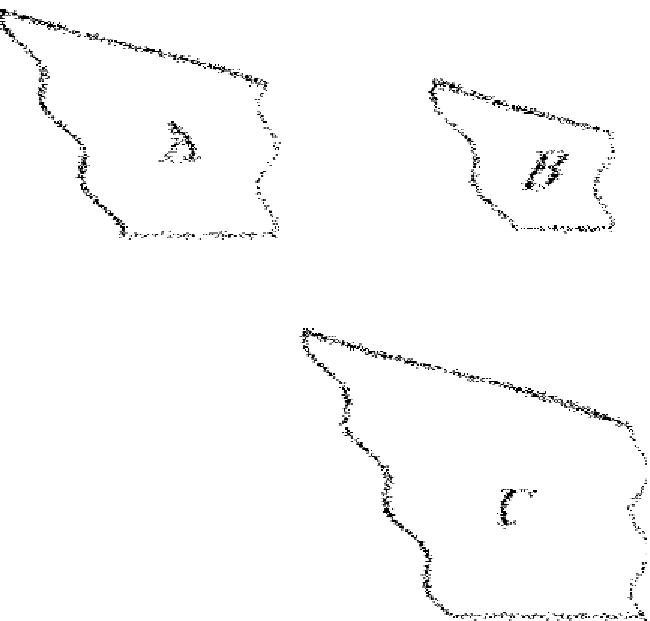
\includegraphics{Book06/front.pdf}}
\newpage

%%%%%%%
% Definitions
%%%%%%%
\pdfbookmark[1]{Definitions}{def6}
\pagestyle{fancy}
\cfoot{\gr{\kern -.7pt }}
\lhead{\large\gr{ΣΤΟΙΘΕΙΩΝ \kern -.7pt {6}.}}
\rhead{\large ELEMENTS BOOK 6}
\begin{Parallel}{}{} 
\ParallelLText{
\begin{center}
\large{\gr{<'Οροι}.}
\end{center}\vspace*{-7pt}

\ggn{1}. ~\gr{<'Ομοια σθήματα εὐθύγραμμά ἐστιν, <όσα τάξ τε γωνίαξ >ίσαξ >έθει
κατὰ μίαν καὶ τὰξ περὶ τὰξ >ίσαξ γωνίαξ πλευρὰξ ἀνάλογον.}

\ggn{2}.~\gr{>'Ακρον καὶ μέσον λόγον εὐθεῖα τετμ\kern -.7pt  ῆσθαι λέγεται, <όταν >ῆ|
ὡξ ἡ <όλη πρὸξ τὸ μεῖζον τμ\kern -.7pt  ῆμα, ο<ύτωξ τὸ μεῖζον
πρὸξ τὸ >έλαττὸν.}

\ggn{3}.~\gr{<'Υψοξ ἐστὶ πάντοξ σθήματοξ ἡ ἀπὸ τῆξ κορυφῆξ
ἐπὶ τὴν βάσιν κάθετοξ ἀγομένη.}}

\ParallelRText{
\begin{center}
{\large Definitions}
\end{center}

1.~Similar rectilinear figures  are those (which) have  (their) angles separately equal, and the (corresponding) sides about the equal angles proportional.

2.~A straight-line is said to be cut in extreme and mean ratio when
as the whole is to the greater segment so the greater (segment is) to the lesser.

3.~The height of any figure is the (straight-line)  drawn
from the vertex perpendicular to the base.}
\end{Parallel}

%%%%%%
% Prop 6.1
%%%%%%
\pdfbookmark[1]{Proposition 6.1}{pdf6.1}
\begin{Parallel}{}{} 
\ParallelLText{
\begin{center}
{\large \ggn{1}.}
\end{center}\vspace*{-7pt}

\gr{Τὰ τρίγωνα καὶ τὰ παραλληλόγραμμα τὰ ὑπὸ τὸ α\kern -.7pt  ὐτὸ <ύψοξ >όντα
πρὸξ >άλληλά ἐστιν ὡξ αἱ βάσειξ.}

% Removed epsf size command
\centerline{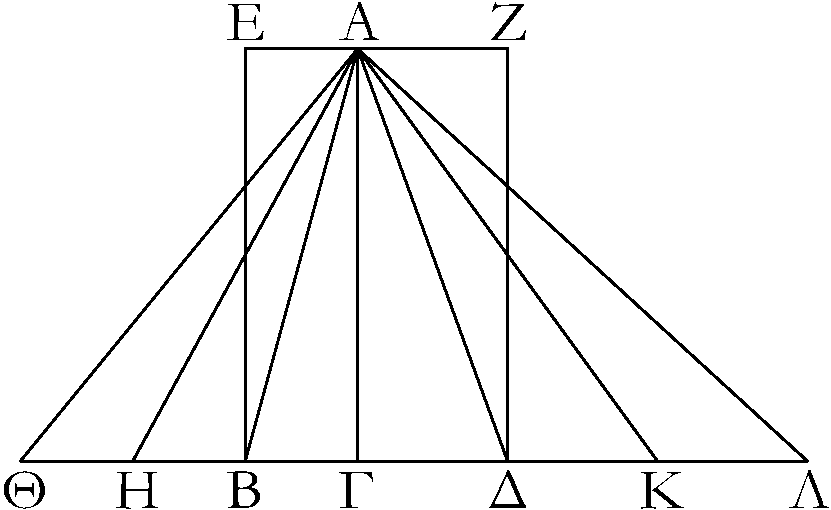
\includegraphics{Book06/fig01g.pdf}}

\gr{>'Εστω τρίγωνα μὲν τὰ ΑΒΓ, ΑΓΔ, παραλληλόγραμ\-μα δὲ τὰ ΕΓ, ΓΖ
ὑπὸ τὸ α\kern -.7pt  ὐτὸ <ύψοξ τὸ ΑΓ; λέγω, <ότι ἐστὶν ὡξ ἡ ΒΓ βάσιξ
πρὸξ τὴν ΓΔ βάσιν, ο<ύτωξ τὸ ΑΒΓ τρίγωνον πρὸξ τὸ ΑΓΔ
τρίγωνον, καὶ τὸ ΕΓ παραλληλόγραμμον πρὸξ τὸ ΓΖ παραλληλόγραμμον.}

\gr{Ἐκβεβλήσθω γὰρ ἡ ΒΔ ἐφ> ἑκάτερα τὰ μέρη ἐπὶ τὰ Θ, Λ
σημεῖα, καὶ κείσθωσαν τῆ| μὲν ΒΓ βάσει  >ίσαι [ὁσαιδηποτοῦν] αἱ ΒΗ, ΗΘ, τῆ|
δὲ ΓΔ βάσει >ίσαι ὁσαιδηποτοῦν αἱ ΔΚ, ΚΛ, καὶ ἐπεζεύθθωσαν
αἱ ΑΗ, ΑΘ, ΑΚ, ΑΛ.}

\gr{Καὶ ἐπεὶ >ίσαι εἰσὶν αἱ ΓΒ, ΒΗ, ΗΘ ἀλλήλαιξ, >ίσα ἐστὶ καὶ τὰ
ΑΘΗ, ΑΗΒ, ΑΒΓ τρίγωνα ἀλλήλοιξ. ὁσαπλασίων >άρα ἐστὶν ἡ
ΘΓ βάσιξ τῆξ ΒΓ βάσεωξ, τοσαυταπλάσιόν ἐστι καὶ τὸ ΑΘΓ τρίγωνον
τοῦ ΑΒΓ τριγώνου. διὰ τὰ α\kern -.7pt  ὐτὰ δὴ ὁσαπλασίων ἐστὶν ἡ ΛΓ βάσιξ
τῆξ ΓΔ βάσεωξ, τοσαυταπλάσιόν ἐστι καὶ τὸ ΑΛΓ τρίγωνον τοῦ
ΑΓΔ τριγώνου; καὶ εἰ >ίση ἐστὶν ἡ ΘΓ βάσιξ τῆ| ΓΛ βάσει, >ίσον
ἐστὶ καὶ τὸ ΑΘΓ τρίγωνον τῳ ΑΓΛ τριγώνῳ, καὶ εἰ ὑπερέθει ἡ ΘΓ βάσιξ τῆξ ΓΛ βάσεωξ, ὑπερέθει καὶ τὸ ΑΘΓ τρίγωνον τοῦ
ΑΓΛ τριγώνου, καὶ εἰ ἐλάσσων,
>έλασσον. τεσσάρων δὴ >όντων μεγεθῶν δύο μὲν βάσεων τῶν
ΒΓ, ΓΔ, δύο δὲ τριγώνων τῶν ΑΒΓ, ΑΓΔ ε>ίληπται ἰσάκιξ
πολλαπλάσια τῆξ μὲν ΒΓ βάσεωξ καὶ τοῦ ΑΒΓ τριγώνου <ή τε
ΘΓ βάσιξ καὶ τὸ  ΑΘΓ τρίγωνον, τῆξ δὲ ΓΔ βάσεωξ καὶ τοῦ ΑΔΓ
τριγώνου >άλλα, <ὰ >έτυθεν, ἰσάκιξ πολλαπλάσια <ή τε
ΛΓ βάσιξ καὶ τὸ ΑΛΓ τρίγωνον; καὶ δέδεικται, <ότι, εἰ ὑπερέθει ἡ
ΘΓ βάσιξ τῆξ ΓΛ βάσεωξ, ὑπερέθει καὶ τὸ ΑΘΓ τρίγωνον τοῦ
ΑΛΓ τριγώνου, καί εἰ >ίση, >ίσον, καὶ εἰ >έλασσων, >έλασσον;
>έστιν >άρα ὡξ ἡ ΒΓ βάσιξ πρὸξ τὴν ΓΔ βάσιν, ο<ύτωξ τὸ ΑΒΓ
τρίγωνον πρὸξ τὸ ΑΓΔ τρίγωνον.}

\gr{Καὶ ἐπεὶ τοῦ μὲν ΑΒΓ τριγώνου διπλάσιόν ἐστι τὸ ΕΓ παραλληλόγραμμον, τοῦ δὲ ΑΓΔ τριγώνου διπλάσιόν ἐστι τὸ ΖΓ
παραλληλόγραμμον, τὰ δὲ μέρη τοῖξ ὡσα\kern -.7pt  ύτωξ πολλαπλασίοιξ τὸν
α\kern -.7pt  ὐτὸν >έθει λόγον, >έστιν >άρα ὡξ τὸ ΑΒΓ τρίγωνον πρὸξ
τὸ ΑΓΔ τρίγωνον, ο<ύτωξ τὸ ΕΓ παραλληλόγραμμον πρὸξ τὸ ΖΓ
παραλληλόγραμμον. ἐπεὶ ο>ῦν ἐδείθθη, ὡξ μὲν ἡ ΒΓ
βάσιξ πρὸξ τὴν ΓΔ, ο<ύτωξ τὸ ΑΒΓ τρίγωνον πρὸξ τὸ ΑΓΔ 
τρίγωνον, ὡξ δὲ τὸ ΑΒΓ τρίγωνον πρὸξ
τὸ ΑΓΔ τρίγωνον, ο<ύτωξ
τὸ ΕΓ παραλληλόγραμμον πρὸξ τὸ ΓΖ παραλληλόγραμμον, καὶ ὡξ >άρα
ἡ ΒΓ βάσιξ πρὸξ τὴν ΓΔ βάσιν, ο<ύτωξ τὸ ΕΓ παραλληλόγραμμον
πρὸξ τὸ ΖΓ παραλληλόγραμμον.}

\gr{Τὰ >άρα  τρίγωνα καὶ τὰ παραλληλόγραμμα τὰ ὑπὸ τὸ α\kern -.7pt  ὐτὸ <ύψοξ >όντα
πρὸξ >άλληλά ἐστιν ὡξ αἱ βάσειξ; <όπερ >έδει δεῖχαι.}}

\ParallelRText{
\begin{center}
{\large Proposition 1}$^\dag$
\end{center}

Triangles and parallelograms which are of the same height are to one another as their bases.

% Removed epsf size command
\centerline{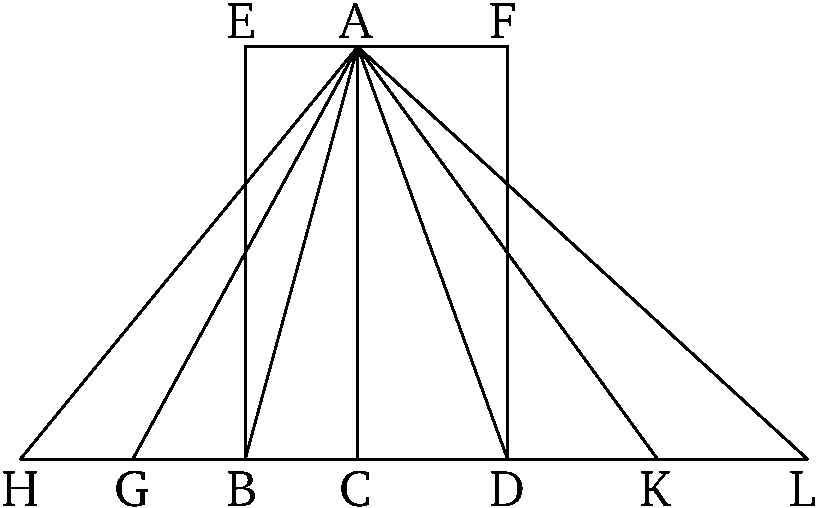
\includegraphics{Book06/fig01e.pdf}}

Let $ABC$ and $ACD$ be triangles, and $EC$ and $CF$ parallelograms, of the same
height $AC$. I say that as  base $BC$ is to  base $CD$, so  triangle
$ABC$ (is) to  triangle $ACD$, and  parallelogram $EC$ to  parallelogram
$CF$.

For let the (straight-line) $BD$ be produced in each direction to points $H$ and $L$, and
let [any number] (of straight-lines) $BG$ and $GH$ be made equal to  base $BC$,
and any number (of straight-lines) $DK$ and $KL$ equal to  base $CD$.
And let $AG$, $AH$, $AK$, and $AL$ be joined.

And since $CB$, $BG$, and $GH$ are equal to one another, triangles
$AHG$, $AGB$, and $ABC$ are also equal to one another  [Prop.~1.38].
Thus, as many times as  base $HC$ is (divisible by)  base $BC$, so many times is  triangle $AHC$ also (divisible) by  triangle $ABC$. So, for
the same (reasons), as many times as  base $LC$ is (divisible) by
 base $CD$, so many times is triangle $ALC$ also (divisible) by 
triangle $ACD$. And if  base $HC$ is equal to base $CL$, (then)
triangle $AHC$ is also equal to  triangle $ACL$  [Prop.~1.38].
And if  base $HC$ exceeds  base $CL$, (then)  triangle
$AHC$ also exceeds triangle $ACL$.$^\ddag$ And if ($HC$ is) less (than 
$CL$ then  $AHC$ is also) less (than $ACL$).
So, their being four magnitudes,  two bases, $BC$ and $CD$, and  two
triangles, $ABC$ and $ACD$, equal multiples have been taken of  base
$BC$ and triangle $ABC$---(namely), base $HC$ and triangle
$AHC$---and other random equal multiples of base $CD$ and 
triangle $ADC$---(namely),  base $LC$ and triangle $ALC$. And it has been
shown that if  base $HC$ exceeds base $CL$, (then)  triangle
$AHC$ also exceeds  triangle $ALC$, and if ($HC$ is) equal (to $CL$ then $AHC$ is also)
equal (to $ALC$), and if ($HC$ is) less (than $CL$ then $AHC$ is also) less (than
$ALC$). Thus, as base $BC$ is to base $CD$, so triangle $ABC$ (is) to
triangle $ACD$ [Def.~5.5].  And since parallelogram $EC$ is double  triangle $ABC$, and parallelogram
$FC$ is double triangle $ACD$  [Prop.~1.34], and parts have the same
ratio as similar multiples [Prop.~5.15], thus
as triangle $ABC$ is to triangle $ACD$, so parallelogram $EC$ (is) to parallelogram
$FC$. In fact, since it was shown that as base $BC$ (is) to $CD$, so
triangle $ABC$ (is) to triangle $ACD$,  and as triangle $ABC$ (is) to triangle $ACD$, so
parallelogram $EC$ (is) to parallelogram $CF$, thus, also, as base $BC$ (is) to
base $CD$, so parallelogram $EC$ (is) to parallelogram $FC$ [Prop.~5.11].

Thus, triangles and parallelograms which are of the same height are to one another as their bases. (Which is) the very thing it was required to show.}
\end{Parallel}
{\footnotesize \noindent$^\dag$ As is easily demonstrated, this proposition
holds even when the triangles, or parallelograms, do not share a common
side, and/or are not right-angled.\\[0.5ex]
$^\ddag$ This is a straight-forward generalization of Prop.~1.38.}

%%%%%%
% Prop 6.2
%%%%%%
\pdfbookmark[1]{Proposition 6.2}{pdf6.2}
\begin{Parallel}{}{} 
\ParallelLText{
\begin{center}
{\large \ggn{2}.}
\end{center}\vspace*{-7pt}

\gr{Ἐὰν τριγώνου παρὰ μίαν τῶν πλευρῶν ἀθθῆ| τιξ εὐθεῖα, ἀνάλογον
τεμεῖ τὰξ τοῦ τριγώνου πλευράξ; καὶ ἒαν αἱ τοῦ τριγώνου πλευραὶ
ἀνάλογον τμ\kern -.7pt  ηθῶσιν, ἡ ἐπὶ τὰξ τομὰξ ἐπιζευγνυμένη εὐθεῖα
παρὰ τὴν λοιπὴν >έσται τοῦ τριγώνου πλευράν.}

% Removed epsf size command
\centerline{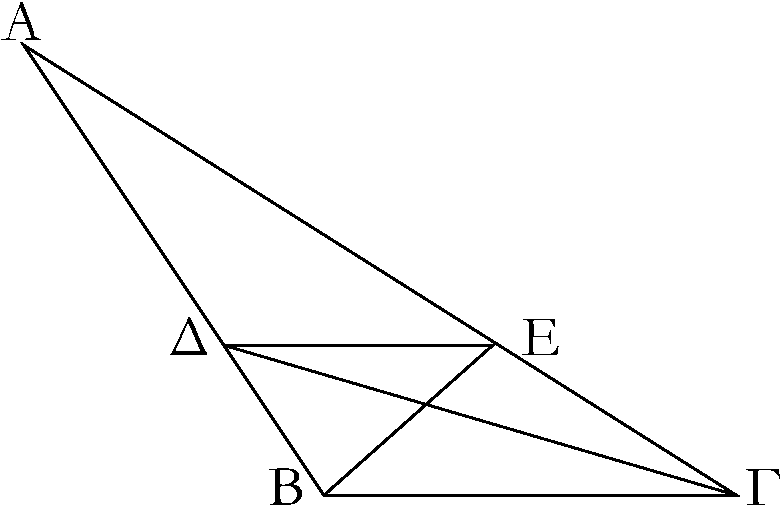
\includegraphics{Book06/fig02g.pdf}}

\gr{Τριγώνου γὰρ τοῦ ΑΒΓ παράλληλοξ μιᾶ| τῶν πλευρῶν τῆ| ΒΓ
>ήθθω ἡ ΔΕ; λέγω, <ότι ἐστὶν ὡξ ἡ ΒΔ πρὸξ τὴν ΔΑ, ο<ύτωξ ἡ ΓΕ
πρὸξ τὴν ΕΑ.}

\gr{Ἐπεζεύθθωσαν γὰρ αἱ ΒΕ, ΓΔ.}

\gr{>'Ισον >άρα ἐστὶ τὸ ΒΔΕ τρίγωνον τῶ| ΓΔΕ τριγώνῳ; ἐπὶ γὰρ τῆξ
α\kern -.7pt  ὐτῆξ βάσεώξ ἐστι τῆξ ΔΕ καὶ ἐν ταῖξ α\kern -.7pt  ὐταῖξ παραλλήλοιξ ταῖξ
ΔΕ, ΒΓ; >άλλο δέ τι τὸ ΑΔΕ τρίγωνον. τὰ δὲ >ίσα πρὸξ τὸ α\kern -.5pt  ὐτὸ
τὸν α\kern -.3pt  ὐτὸν >έθει λόγον; >έστιν >άρα ὡξ τὸ ΒΔΕ τρίγωνον
πρὸξ τὸ ΑΔΕ [τρίγωνον], ο<ύτωξ τὸ ΓΔΕ τρίγωνον πρὸξ τὸ ΑΔΕ τρίγωνον. αλλ> ὡξ μὲν τὸ ΒΔΕ τρίγωνον πρὸξ τὸ ΑΔΕ, ο<ύτωξ ἡ
ΒΔ πρὸξ τὴν ΔΑ; ὑπὸ γὰρ τὸ α\kern -.7pt  ὐτὸ <ύψοξ >όντα τὴν ἀπὸ τοῦ
Ε ἐπὶ τὴν ΑΒ κάθετον ἀγομένην πρὸξ >άλληλά εἰσιν ὡξ αἱ
βάσειξ. διὰ τὰ α\kern -.7pt  ὐτὰ δὴ ὡξ τὸ ΓΔΕ τρίγωνον πρὸξ τὸ ΑΔΕ, ο<ύτωξ
ἡ ΓΕ πρὸξ τὴν ΕΑ; καὶ ὡξ >άρα ἡ ΒΔ πρὸξ τὴν ΔΑ, ο<ύτωξ ἡ ΓΕ
πρὸξ τὴν ΕΑ.}

\gr{Ἀλλὰ δὴ αἱ τοῦ ΑΒΓ τριγώνου πλευραὶ αἱ ΑΒ, ΑΓ ἀνάλογον
τετμ\kern -.7pt  ήσθωσαν, ὡξ ἡ ΒΔ πρὸξ τὴν ΔΑ, ο<ύτωξ ἡ ΓΕ πρὸξ τὴν
ΕΑ, καὶ ἐπεζεύθθω ἡ ΔΕ; λέγω, <ότι παράλληλόξ ἐστιν ἡ ΔΕ
τῆ| ΒΓ.}

\gr{Τῶν γὰρ α\kern -.7pt  ὐτῶν κατασκευασθέντων, ἐπεί ἐστιν ὡξ ἡ ΒΔ πρὸξ
τὴν ΔΑ, ο<ύτωξ ἡ ΓΕ πρὸξ τὴν ΕΑ, ἀλλ> ὡξ μὲν ἡ ΒΔ πρὸξ τὴν
ΔΑ, ο<ύτωξ τὸ ΒΔΕ τρίγωνον πρὸξ τὸ ΑΔΕ τρίγωνον, ὡξ δὲ ἡ ΓΕ
πρὸξ τὴν ΕΑ, ο<ύτωξ τὸ ΓΔΕ τρίγωνον πρὸξ τὸ ΑΔΕ τρίγωνον, καὶ
ὡξ >άρα τὸ ΒΔΕ τρίγωνον πρὸξ τὸ  ΑΔΕ τρίγωνον, ο<ύτωξ τὸ ΓΔΕ
τρίγωνον πρὸξ τὸ ΑΔΕ τρίγωνον. ἑκάτερον >άρα τῶν ΒΔΕ, ΓΔΕ
τριγώνων πρὸξ τὸ ΑΔΕ τὸν α\kern -.7pt  ὐτὸν >έθει λόγον. >ίσον
>άρα ἐστὶ τὸ ΒΔΕ τρίγωνον τῶ| ΓΔΕ τριγώνῳ; καί εἰσιν ἐπὶ τῆξ
α\kern -.5pt  ὐτῆξ βάσεωξ τῆξ ΔΕ. τὰ δὲ >ίσα τρίγωνα καὶ ἐπὶ τῆξ α\kern -.3pt  ὐτῆξ
βάσεωξ >όντα καὶ ἐν ταῖξ α\kern -.7pt  ὐταῖξ παραλλήλοιξ ἐστίν. παράλληλοξ
>άρα ἐστὶν ἡ ΔΕ τῆ| ΒΓ.}

\gr{Ἐὰν >άρα τριγώνου παρὰ μίαν τῶν πλευρῶν ἀθθῆ| τιξ εὐθεῖα, ἀνάλογον
τεμεῖ τὰξ τοῦ τριγώνου πλευράξ; καὶ ἒαν αἱ τοῦ τριγώνου πλευραὶ
ἀνάλογον τμ\kern -.7pt  ηθῶσιν, ἡ ἐπὶ τὰξ τομὰξ ἐπιζευγνυμένη εὐθεῖα
παρὰ τὴν λοιπὴν >έσται τοῦ τριγώνου πλευράν; <όπερ >έδει
δεῖχαι.}}

\ParallelRText{
\begin{center}
{\large Proposition 2}
\end{center}

If some straight-line is drawn parallel to one of the
sides of a triangle, (then) it will cut the (other) sides of the triangle
proportionally. And if (two of) the sides of a triangle are cut proportionally, (then)
the straight-line joining the cutting (points) will be parallel to the remaining side of the
triangle.

% Removed epsf size command
\centerline{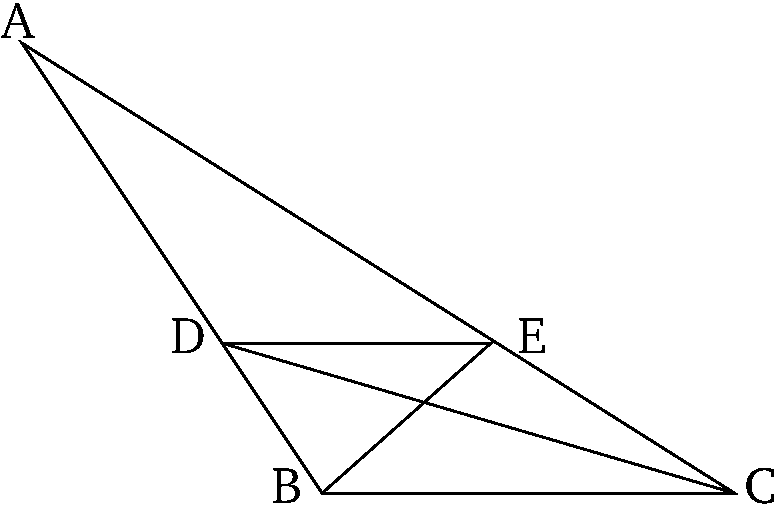
\includegraphics{Book06/fig02e.pdf}}

For let $DE$ be drawn parallel to one of the sides $BC$ of triangle $ABC$.
I say that as $BD$ is to $DA$, so $CE$ (is) to $EA$.

For let $BE$ and $CD$ be joined.

Thus, triangle $BDE$ is equal to triangle $CDE$. For they are on the same
base $DE$ and between the same parallels $DE$ and $BC$  [Prop.~1.38].
And $ADE$ is some other triangle. And equal (magnitudes)
have the same ratio to the same (magnitude) [Prop.~5.7]. Thus, as triangle $BDE$ is to [triangle]
$ADE$, so triangle $CDE$ (is) to triangle $ADE$. But, as triangle $BDE$ (is) to
triangle $ADE$, so (is) $BD$ to $DA$. For, having the same height---(namely), the
(straight-line) drawn from $E$ perpendicular to $AB$---they are to one another as their bases
[Prop.~6.1].
So, for the same (reasons), as triangle $CDE$ (is) to $ADE$, so $CE$ (is) to $EA$.
And, thus, as $BD$ (is) to $DA$, so $CE$ (is) to $EA$ [Prop.~5.11].

And so, let the sides $AB$ and $AC$ of triangle $ABC$ be cut proportionally (such that)
as $BD$ (is) to $DA$, so $CE$ (is) to $EA$. And let $DE$ be joined. I say that
$DE$ is parallel to $BC$.

For, by the same construction, since as $BD$ is to $DA$, so $CE$ (is) to $EA$, but
as $BD$ (is) to $DA$, so triangle $BDE$ (is) to triangle $ADE$, and as $CE$
(is) to $EA$, so triangle $CDE$ (is) to triangle $ADE$ [Prop.~6.1], thus, also,  as triangle $BDE$ (is) to triangle
$ADE$, so triangle $CDE$ (is) to triangle $ADE$ [Prop.~5.11]. Thus, triangles $BDE$ and $CDE$ each have the same ratio to $ADE$. Thus, triangle $BDE$ is equal to triangle $CDE$ [Prop.~5.9].
And they are on the same base $DE$. And equal triangles, which are also on the same base, are also between the same parallels  [Prop.~1.39]. Thus,
$DE$ is parallel to $BC$.

Thus, if some straight-line is drawn parallel to one of the
sides of a triangle, (then) it will cut the (other) sides of the triangle
proportionally. And if (two of) the sides of a triangle are cut proportionally, (then)
the straight-line joining the cutting (points) will be parallel to the remaining side of the
triangle. (Which is) the very thing it was required to show.}
\end{Parallel}

%%%%%%
% Prop 6.3
%%%%%%
\pdfbookmark[1]{Proposition 6.3}{pdf6.3}
\begin{Parallel}{}{} 
\ParallelLText{
\begin{center}
{\large \ggn{3}.}
\end{center}\vspace*{-7pt}

\gr{Ἐὰν τριγώνου ἡ γωνία δίθα τμ\kern -.7pt  ηθῆ|, ἡ δὲ τέμνουσα τὴν γωνίαν
εὐθεῖα τέμνῃ καὶ τὴν βάσιν, τὰ τῆξ βάσεωξ τμ\kern -.7pt  ήματα τὸν 
α\kern -.5pt  ὐτὸν <έχει λόγον ταῖξ λοιπαῖξ τοῦ τριγώνου πλευραῖξ;
καὶ ἒαν τὰ τῆξ βάσεωξ τμ\kern -.3pt  ήματα τὸν α\kern -.7pt  ὐτὸν >έθῃ λόγον
ταῖξ λοιπαῖξ τοῦ τριγώνου πλευραῖξ, ἡ ἀπὸ τῆξ κορυφῆξ ἐπὶ
τὴν τομ\kern -.7pt  ὴν ἐπιζευγνυμένη εὐθεῖα δίθα τεμεῖ τὴν τοῦ
τριγώνου γωνίαν.}

\gr{>'Εστω τρίγωνον τὸ ΑΒΓ, καὶ τετμ\kern -.7pt  ήσθω ἡ ὑπὸ ΒΑΓ γωνία δίθα
ὑπὸ τῆξ ΑΔ εὐθείαξ; λέγω, <ότι ἐστὶν ὡξ ἡ ΒΔ πρὸξ τὴν
ΓΔ, ο<ύτωξ ἡ ΒΑ πρὸξ τὴν ΑΓ.}

\gr{>'Ηθθω γὰρ διὰ τοῦ Γ τῆ| ΔΑ παράλληλοξ ἡ ΓΕ, καὶ διαθθεῖσα
ἡ ΒΑ συμπιπτέτω α\kern -.7pt  ὐτῆ| κατὰ τὸ Ε.}

\gr{Καὶ ἐπεὶ εἰξ παραλλήλουξ τὰξ ΑΔ, ΕΓ εὐθεῖα ἐνέπεσεν ἡ
ΑΓ, ἡ >άρα ὑπὸ ΑΓΕ γωνία >ίση ἐστὶ τῆ| ὑπὸ ΓΑΔ.
ἀλλ> ἡ ὑπὸ ΓΑΔ τῆ| ὑπὸ ΒΑΔ ὑπόκειται >ίση; καὶ ἡ ὑπὸ
ΒΑΔ >άρα τῆ| ὑπὸ
ΑΓΕ ἐστιν >ίση. πάλιν, ἐπεὶ εἰξ
παραλλήλουξ τὰξ ΑΔ, ΕΓ εὐθεῖα ἐνέπεσεν ἡ ΒΑΕ, ἡ ἐκτὸξ
γωνία ἡ ὑπὸ ΒΑΔ >ίση ἐστὶ τῆ| ἐντὸξ τῆ| ὑπὸ ΑΕΓ.
ἐδείθθη δὲ καὶ ἡ ὑπὸ ΑΓΕ τῆ| ὑπὸ ΒΑΔ >ίση; καὶ ἡ
ὑπὸ ΑΓΕ >άρα γωνία τῆ| ὑπὸ ΑΕΓ ἐστιν >ίση; <ώστε καὶ
πλευρὰ ἡ ΑΕ πλευρᾶ| τῆ| ΑΓ ἐστιν >ίση. καὶ ἐπεὶ τριγώνου
τοῦ ΒΓΕ παρὰ μίαν τῶν πλευρῶν τὴν ΕΓ >ῆκται ἡ
ΑΔ, ἀνάλογον >άρα ἐστὶν ὡξ ἡ ΒΔ πρὸξ τὴν ΔΓ, ο<ύτωξ
ἡ ΒΑ πρὸξ τὴν ΑΕ. >ίση δὲ ἡ ΑΕ τῆ| ΑΓ; ὡξ >άρα ἡ ΒΔ
πρὸξ τὴν ΔΓ, ο<ύτωξ ἡ ΒΑ πρὸξ τὴν ΑΓ.}\\~\\

% Removed epsf size command
\centerline{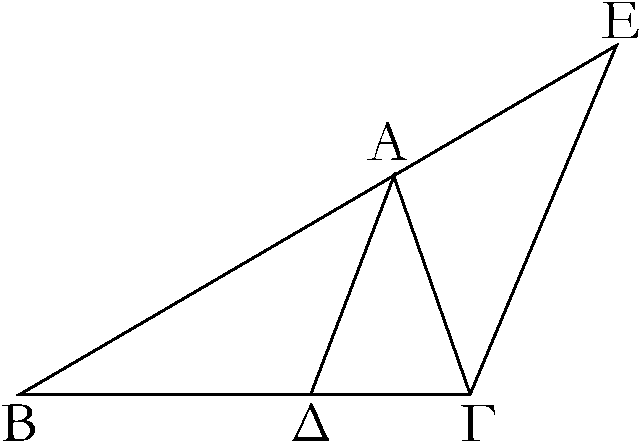
\includegraphics{Book06/fig03g.pdf}}

\gr{Ἀλλὰ δὴ >έστω ὡξ ἡ ΒΔ πρὸξ τὴν ΔΓ, ο<ύτωξ ἡ ΒΑ
πρὸξ τὴν ΑΓ, καὶ ἐπεζεύθθω ἡ ΑΔ; λέγω, <ότι δίθα
τέτμ\kern -.7pt  ηται ἡ ὑπὸ ΒΑΓ γωνία ὑπὸ τῆξ ΑΔ εὐθείαξ.}

\gr{Τῶν γὰρ α\kern -.7pt  ὐτῶν κατασκευασθέντων, ἐπεί ἐστιν ὡξ ἡ ΒΔ
πρὸξ τὴν ΔΓ, ο<ύτωξ ἡ ΒΑ πρὸξ τὴν ΑΓ, ἀλλὰ καὶ ὡξ ἡ
ΒΔ πρὸξ τὴν ΔΓ, ο<ύτωξ ἐστὶν ἡ ΒΑ πρὸξ τὴν ΑΕ; τριγώνου
γὰρ τοῦ ΒΓΕ παρὰ μίαν τὴν ΕΓ >ῆκται ἡ ΑΔ; καὶ ὡξ >άρα
ἡ ΒΑ πρὸξ τὴν ΑΓ, ο<ύτωξ ἡ ΒΑ πρὸξ τὴν ΑΕ. >ίση >άρα
ἡ ΑΓ τῆ| ΑΕ; <ώστε καὶ γωνία ἡ ὑπὸ ΑΕΓ τῆ| ὑπὸ
ΑΓΕ ἐστιν >ίση. ἀλλ> ἡ μὲν ὑπὸ ΑΕΓ τῆ| ἐκτὸξ τῆ|
ὑπὸ ΒΑΔ [ἐστιν] >ίση, ἡ δὲ ὑπὸ ΑΓΕ τῆ| ἐναλλὰχ
τῆ| ὑπὸ ΓΑΔ ἐστιν >ίση; καὶ ἡ ὑπὸ ΒΑΔ >άρα τῆ| ὑπὸ
ΓΑΔ ἐστιν >ίση. ἡ >άρα ὑπὸ ΒΑΓ γωνία δίθα τέτμ\kern -.7pt  ηται
ὑπὸ τῆξ ΑΔ εὐθείαξ.}

\gr{Ἐὰν >άρα τριγώνου ἡ γωνία δίθα τμ\kern -.7pt  ηθῆ|, ἡ δὲ τέμνουσα τὴν γωνίαν
εὐθεῖα τέμνῃ καὶ τὴν βάσιν, τὰ τῆξ βάσεωξ τμ\kern -.7pt  ήματα τὸν 
α\kern -.5pt  ὐτὸν <έχει λόγον ταῖξ λοιπαῖξ τοῦ τριγώνου πλευραῖξ;
καὶ ἒαν τὰ τῆξ βάσεωξ τμ\kern -.3pt  ήματα τὸν α\kern -.7pt  ὐτὸν >έθῃ λόγον
ταῖξ λοιπαῖξ τοῦ τριγώνου πλευραῖξ, ἡ ἀπὸ τῆξ κορυφῆξ ἐπὶ
τὴν τομ\kern -.7pt  ὴν ἐπιζευγνυμένη εὐθεῖα δίθα τέμνει τὴν τοῦ
τριγώνου γωνίαν; <όπερ >έδει δεῖχαι.}}

\ParallelRText{
\begin{center}
{\large Proposition 3}
\end{center}

If an angle of a triangle is cut in half, and the
straight-line cutting the angle also cuts the base, (then) the segments of the base
will have the same ratio as the remaining sides of the triangle. And if
the segments of the base have the same ratio as the remaining sides of the
triangle, (then) the straight-line joining the vertex to the cutting (point) will
cut the angle of the triangle in half.

Let $ABC$ be a triangle. And let the angle $BAC$ be cut in half
by the straight-line $AD$. I say that as $BD$ is to $CD$, so $BA$ (is) to $AC$.

For let $CE$ be drawn through (point) $C$ parallel to $DA$.  And, $BA$ being drawn
through, let it meet ($CE$) at (point) $E$.$^\dag$

And since the straight-line $AC$ falls across the parallel (straight-lines)
$AD$ and $EC$, angle $ACE$ is thus equal to $CAD$  [Prop.~1.29].
But, (angle) $CAD$ is assumed (to be) equal to $BAD$. Thus, (angle)
$BAD$ is also equal to $ACE$. Again, since the straight-line $BAE$ falls
across the parallel (straight-lines) $AD$ and $EC$, the external angle $BAD$
is equal to the internal (angle) $AEC$  [Prop.~1.29]. And (angle)
$ACE$ was also shown (to be) equal to $BAD$. Thus, angle $ACE$ is also
equal to $AEC$. And, hence, side $AE$ is equal to side $AC$  [Prop.~1.6].
And since $AD$ has been drawn parallel to one of the sides $EC$ of triangle
$BCE$, thus, proportionally, as $BD$ is to $DC$, so $BA$ (is) to $AE$ [Prop.~6.2]. And $AE$ (is) equal to $AC$.
Thus, as $BD$ (is) to $DC$, so $BA$ (is) to $AC$.

% Removed epsf size command
\centerline{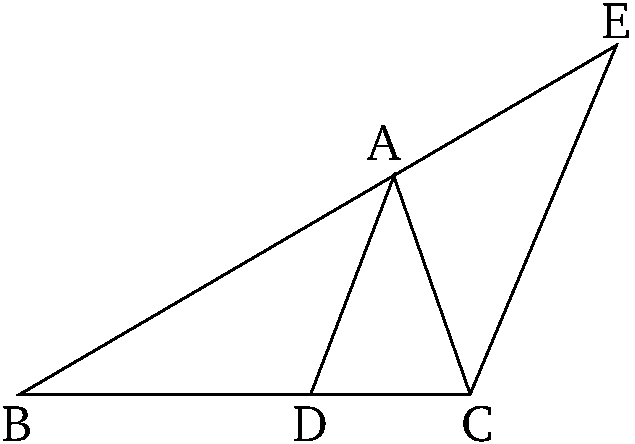
\includegraphics{Book06/fig03e.pdf}}

And so, let $BD$ be to $DC$,  as $BA$ (is) to
$AC$. And let $AD$ be joined. I say that angle $BAC$ has been cut in
half by the straight-line $AD$.

For, by the same construction, since as $BD$ is to $DC$, so $BA$ (is) to
$AC$, (then) also as $BD$ (is) to $DC$, so $BA$ is to $AE$. For $AD$ has been drawn
parallel to one (of the sides) $EC$ of triangle $BCE$ [Prop.~6.2]. Thus, also, as $BA$ (is) to $AC$,
so $BA$ (is) to $AE$  [Prop.~5.11]. Thus,
$AC$ (is) equal to $AE$ [Prop.~5.9].
And, hence, angle $AEC$ is equal to $ACE$  [Prop.~1.5]. But, 
$AEC$ [is] equal to the external (angle) $BAD$, and $ACE$ is equal to the alternate
(angle) $CAD$  [Prop.~1.29]. Thus, (angle) $BAD$ is
also equal to $CAD$. Thus, angle $BAC$ has been cut in half by the
straight-line $AD$.

Thus, if an angle of a triangle is cut in half, and the
straight-line cutting the angle also cuts the base, (then) the segments of the base
will have the same ratio as the remaining sides of the triangle. And if
the segments of the base have the same ratio as the remaining sides of the
triangle, (then) the straight-line joining the vertex to the cutting (point) will
cut the angle of the triangle in half. (Which is) the very thing it was required
to show.}
\end{Parallel}
{\footnotesize \noindent$^\dag$ The fact that the
two straight-lines meet follows because the sum of $ACE$ and $CAE$
is less than two right-angles, as can easily be demonstrated. See Post.~5.}

%%%%%%
% Prop 6.4
%%%%%%
\pdfbookmark[1]{Proposition 6.4}{pdf6.4}
\begin{Parallel}{}{} 
\ParallelLText{
\begin{center}
{\large \ggn{4}.}
\end{center}\vspace*{-7pt}

\gr{Τῶν ἰσογωνίων τριγώνων ἀνάλογόν εἰσιν αἱ πλευραὶ αἱ περὶ τὰξ
>ίσαξ
γωνίαξ καὶ ὁμόλογοι αἱ ὑπὸ τὰξ >ίσαξ γωνίαξ ὑποτείνουσαι.}

\gr{>'Εστω ἰσογώνια τρίγωνα τὰ ΑΒΓ, ΔΓΕ >ίσην >έθοντα τὴν μὲν
ὑπὸ ΑΒΓ γωνίαν τῆ| ὑπὸ ΔΓΕ, τὴν δὲ ὑπὸ ΒΑΓ τῆ| ὑπὸ
ΓΔΕ καὶ >έτι τὴν ὑπὸ ΑΓΒ τῆ| ὑπὸ ΓΕΔ; λέγω, <ότι τῶν
ΑΒΓ, ΔΓΕ τριγώνων ἀνάλογόν εἰσιν αἱ πλευραὶ αἱ περὶ τὰξ >ίσαξ
γωνίαξ καὶ ὁμόλογοι αἱ ὑπὸ τὰξ >ίσαξ γωνίαξ ὑποτείνουσαι.}

\gr{Κείσθω γὰρ ἐπ> εὐθείαξ ἡ ΒΓ τῆ| ΓΕ. καὶ ἐπεὶ αἱ ὑπὸ ΑΒΓ,
ΑΓΒ γωνίαι δύο ὀρθῶν ἐλάττονέξ εἰσιν, >ίση δὲ ἡ ὑπὸ ΑΓΒ τῆ|
ὑπὸ ΔΕΓ, αἱ >άρα ὑπὸ ΑΒΓ, ΔΕΓ δύο ὀρθῶν ἐλάττονέξ εἰσιν;
αἱ ΒΑ, ΕΔ >άρα ἐκβαλλόμεναι συμπεσοῦνται. ἐκβεβλήσθωσαν
καὶ συμπιπτέτωσαν κατὰ τὸ Ζ.}

% Removed epsf size command
\centerline{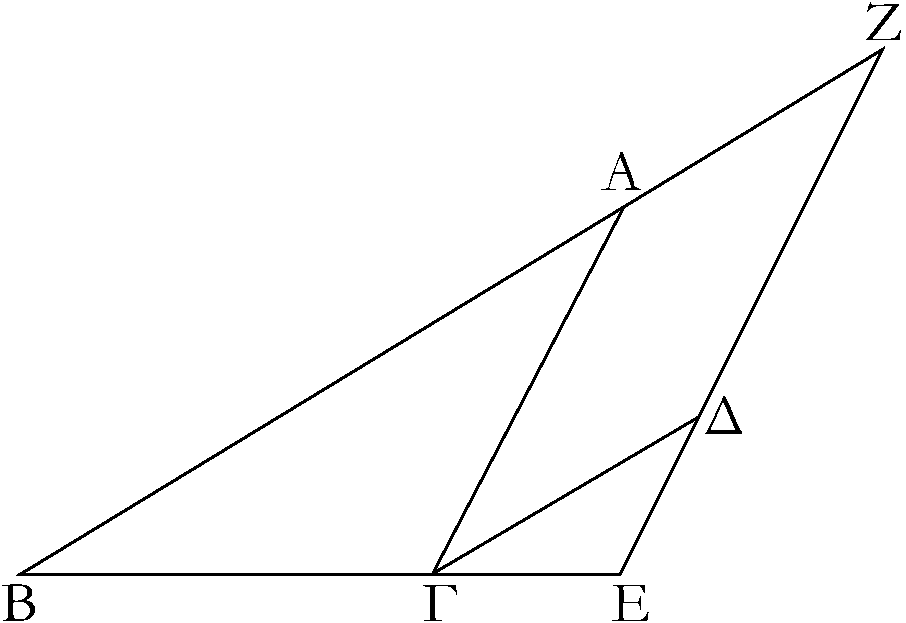
\includegraphics{Book06/fig04g.pdf}}

\gr{Καὶ ἐπεὶ >ίση ἐστὶν ἡ ὑπὸ ΔΓΕ γωνία τῆ| ὑπὸ ΑΒΓ, παράλληλόξ
ἐστιν ἡ ΒΖ τῆ| ΓΔ. πάλιν, ἐπεὶ >ίση ἐστὶν ἡ ὑπὸ ΑΓΒ
τῆ| ὑπὸ ΔΕΓ, παράλληλόξ ἐστιν ἡ
ΑΓ τῆ| ΖΕ. παραλληλόγραμμον >άρα ἐστὶ τὸ ΖΑΓΔ; >ίση >άρα ἡ μὲν ΖΑ τῆ|
ΔΓ, ἡ δὲ ΑΓ τῆ| ΖΔ. καὶ ἐπεὶ τριγώνου τοῦ ΖΒΕ παρὰ μίαν
τὴν ΖΕ >ῆκται ἡ ΑΓ, ἐστιν >άρα ὡξ ἡ ΒΑ πρὸξ τὴν ΑΖ,
ο<ύτωξ ἡ ΒΓ πρὸξ τὴν ΓΕ. >ίση δὲ ἡ ΑΖ τῆ| ΓΔ; ὡξ >άρα
ἡ ΒΑ πρὸξ τὴν ΓΔ, ο<ύτωξ ἡ ΒΓ πρὸξ τὴν ΓΕ, καὶ ἐναλλὰχ ὡξ
ἡ ΑΒ πρὸξ τὴν ΒΓ, ο<ύτωξ ἡ ΔΓ πρὸξ τὴν ΓΕ. πάλιν, ἐπεὶ παράλληλόξ ἐστιν ἡ ΓΔ τῆ| ΒΖ, >έστιν >άρα ὡξ ἡ ΒΓ πρὸξ τὴν
ΓΕ, ο<ύτωξ ἡ ΖΔ πρὸξ τὴν ΔΕ. >ίση δὲ ἡ ΖΔ τῆ| ΑΓ; ὡξ >άρα
ἡ ΒΓ πρὸξ τὴν ΓΕ, ο<ύτωξ ἡ ΑΓ πρὸξ τὴν ΔΕ, καὶ ἐναλλὰχ ὡξ
ἡ ΒΓ πρὸξ τὴν ΓΑ, ο<ύτωξ ἡ ΓΕ πρὸξ τὴν ΕΔ. ἐπεὶ ο>ῦν ἐδείθθη ὡξ μὲν ἡ ΑΒ πρὸξ τὴν ΒΓ, ο<ύτωξ ἡ  ΔΓ πρὸξ τὴν ΓΕ,
ὡξ δὲ ἡ ΒΓ πρὸξ τὴν ΓΑ, ο<ύτωξ ἡ ΓΕ πρὸξ τὴν ΕΔ, δι>
>ίσου >άρα ὡξ ἡ ΒΑ πρὸξ τὴν ΑΓ, ο<ύτωξ ἡ ΓΔ πρὸξ τὴν ΔΕ.}

\gr{Τῶν >άρα ἰσογωνίων τριγώνων ἀνάλογόν εἰσιν αἱ πλευραὶ αἱ περὶ τὰξ
>ίσαξ
γωνίαξ καὶ ὁμόλογοι αἱ ὑπὸ τὰξ >ίσαξ γωνίαξ ὑποτείνουσαι; <όπερ
>έδει δεῖχαι.}}

\ParallelRText{
\begin{center}
{\large Proposition 4}
\end{center}

In equiangular triangles the sides about the
equal angles are proportional, and those (sides) subtending equal angles
 correspond.
 
Let $ABC$ and $DCE$ be equiangular triangles, having angle $ABC$ equal to
$DCE$, and (angle) $BAC$ to $CDE$, and, further,  (angle) $ACB$ to $CED$.
I say that  in triangles $ABC$ and $DCE$ the sides about the equal angles
are proportional, and those (sides) subtending equal angles
 correspond.
 
Let $BC$ be placed straight-on to $CE$. And since angles
$ABC$ and $ACB$ are less than two right-angles  [Prop~1.17], and
$ACB$ (is) equal to $DEC$, thus $ABC$ and $DEC$ are less than two right-angles.
Thus, $BA$ and $ED$, being produced, will meet  [C.N.~5]. Let them be produced,
and let them meet at (point) $F$.

% Removed epsf size command
\centerline{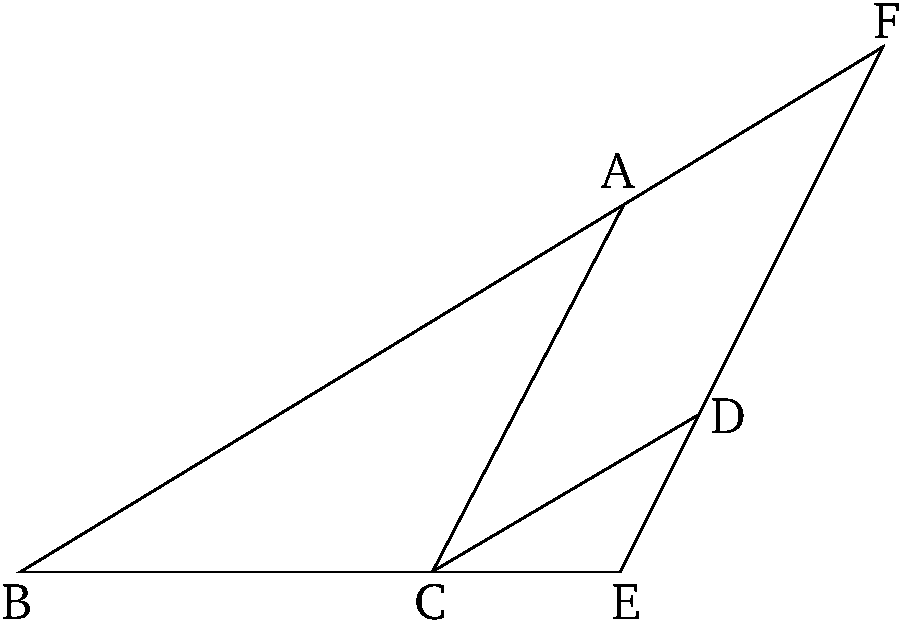
\includegraphics{Book06/fig04e.pdf}}

And since angle $DCE$ is equal to $ABC$, $BF$ is parallel to $CD$  [Prop.~1.28]. Again, since (angle) $ACB$ is equal to $DEC$,  $AC$ is
 parallel to $FE$  [Prop.~1.28]. Thus, $FACD$ is a parallelogram.
Thus, $FA$ is equal to $DC$, and $AC$ to $FD$  [Prop.~1.34]. And since
$AC$ has been drawn parallel to one (of the sides) $FE$ of triangle
$FBE$, thus as $BA$ is to $AF$, so $BC$ (is) to $CE$ [Prop.~6.2]. And $AF$ (is) equal to $CD$.
Thus, as $BA$ (is) to $CD$, so $BC$ (is) to $CE$, and, alternately, as $AB$
(is) to $BC$, so $DC$ (is) to $CE$ [Prop.~5.16].
Again, since $CD$ is parallel to $BF$, thus as $BC$ (is) to $CE$, so
$FD$ (is) to $DE$ [Prop.~6.2]. And $FD$ (is) equal to
$AC$. Thus, as $BC$ is to $CE$, so $AC$ (is) to $DE$, and, alternately, as $BC$ (is)
to $CA$, so $CE$ (is) to $ED$ [Prop.~6.2].
Therefore, since
it was shown that as $AB$ (is) to $BC$, so $DC$ (is) to $CE$, and
as $BC$ (is) to $CA$, so $CE$ (is) to $ED$, thus, via equality, as
$BA$ (is) to $AC$, so $CD$ (is) to $DE$ [Prop.~5.22].

Thus, in  equiangular triangles the sides about the
equal angles are proportional, and those (sides) subtending equal angles
 correspond. (Which is) the very thing it was required to show.}
\end{Parallel}

%%%%%%
% Prop 6.5
%%%%%%
\pdfbookmark[1]{Proposition 6.5}{pdf6.5}
\begin{Parallel}{}{} 
\ParallelLText{
\begin{center}
{\large \ggn{5}.}
\end{center}\vspace*{-7pt}

\gr{Ἐὰν δύο τρίγωνα τὰξ πλευρὰξ ἀνάλογον >έθῃ, ἰσογώνια
>έσται τὰ τρίγωνα καὶ >ίσαξ <έχει τὰξ γωνίαξ, ὑφ> <ὰξ αἱ
ὁμόλογοι πλευραὶ ὑποτείνουσιν.}

\gr{>'Εστω δύο τρίγωνα τὰ ΑΒΓ, ΔΕΖ τὰξ πλευρὰξ ἀνάλογον >έθοντα,
ὡξ μὲν τὴν ΑΒ πρὸξ τὴν ΒΓ, ο<ύτωξ τὴν ΔΕ πρὸξ τὴν
ΕΖ, ὡξ δὲ τὴν ΒΓ πρὸξ τὴν ΓΑ, ο<ύτωξ τὴν ΕΖ πρὸξ τὴν 
ΖΔ, καὶ >έτι ὡξ τὴν ΒΑ πρὸξ τὴν ΑΓ, ο<ύτωξ τὴν ΕΔ πρὸξ τὴν
ΔΖ. λέγω, <ότι ἰσογώνιόν ἐστι τὸ ΑΒΓ τρίγωνον τῶ|
ΔΕΖ τριγώνῳ καὶ >ίσαξ <έχουσι τὰξ γωνίαξ, ὑφ> <ὰξ
αἱ ὁμόλογοι πλευραὶ ὑποτείνουσιν, τὴν μὲν ὑπὸ ΑΒΓ
τῆ| ὑπὸ ΔΕΖ, τὴν δὲ ὑπὸ ΒΓΑ τῆ| ὑπὸ ΕΖΔ καὶ >έτι τὴν
ὑπὸ ΒΑΓ τῆ| ὑπὸ ΕΔΖ.}

\gr{Συνεστάτω γὰρ πρὸξ τῆ| ΕΖ εὐθείᾳ καὶ τοῖξ πρὸξ
α\kern -.7pt  ὐτῆ| σημείοιξ τοῖξ Ε, Ζ τῆ| μὲν ὑπὸ ΑΒΓ γωνίᾳ
>ίση ἡ ὑπὸ ΖΕΗ, τῆ| δὲ ὑπὸ ΑΓΒ >ίση ἡ ὑπὸ
ΕΖΗ; λοιπὴ >άρα ἡ πρὸξ τῶ| Α λοιπῆ| τῆ| πρὸξ τῶ| Η ἐστιν
>ίση.}

% Removed epsf size command
\centerline{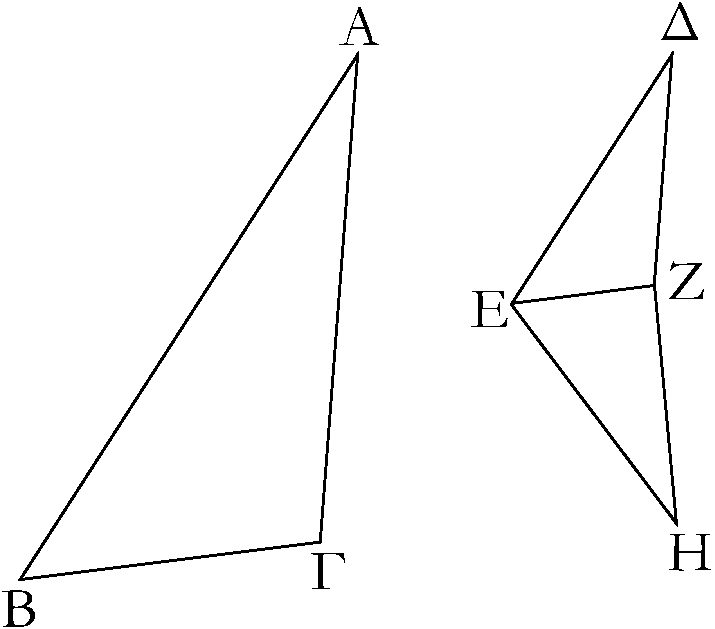
\includegraphics{Book06/fig05g.pdf}}

\gr{>'Ισογώνιον >άρα ἐστὶ τὸ ΑΒΓ τρίγωνον τῶ| ΕΗΖ [τριγών\-ῳ].
τῶν >άρα ΑΒΓ, ΕΗΖ τριγώνων ἀνάλογόν εἰσιν αἱ πλευραὶ
αἱ περὶ τὰξ >ίσαξ γωνίαξ καὶ ὁμόλογοι αἱ ὑπὸ τὰξ >ίσαξ γωνίαξ
ὑποτείνουσαι; >έστιν >άρα ὡξ ἡ ΑΒ πρὸξ τὴν ΒΓ, [ο<ύτωξ]
ἡ ΗΕ πρὸξ τὴν ΕΖ. ἀλλ> ὡξ ἡ ΑΒ πρὸξ τὴν ΒΓ, ο<ύτωξ
ὑπόκειται ἡ ΔΕ πρὸξ τὴν ΕΖ; ὡξ >άρα ἡ ΔΕ πρὸξ τὴν ΕΖ,
ο<ύτωξ ἡ ΗΕ πρὸξ τὴν ΕΖ. ἑκατέρα >άρα τῶν ΔΕ, ΗΕ πρὸξ τὴν
ΕΖ τὸν α\kern -.7pt  ὐτὸν >έθει λόγον; >ίση >άρα ἐστὶν ἡ ΔΕ τῆ| ΗΕ. διὰ
τὰ α\kern -.7pt  ὐτὰ δὴ καὶ ἡ ΔΖ τῆ| ΗΖ ἐστιν >ίση. ἐπεὶ  ο>ῦν >ίση
ἐστὶν ἡ ΔΕ τῆ| ΕΗ, κοινὴ δὲ ἡ ΕΖ, δύο δὴ αἱ ΔΕ, ΕΖ δυσὶ
ταῖξ ΗΕ, ΕΖ >ίσαι εἰσίν; καὶ βάσιξ ἡ ΔΖ βάσει τῆ| ΖΗ
[ἐστιν] >ίση; γωνία >άρα ἡ ὑπὸ ΔΕΖ γωνίᾳ τῆ| ὑπὸ ΗΕΖ
ἐστιν >ίση, καὶ τὸ ΔΕΖ
τρίγωνον τῶ| ΗΕΖ τριγώνῳ
>ίσον, καὶ αἱ λοιπαὶ γωνίαι ταῖξ λοιπαῖξ
γωνίαιξ >ίσαι, ὑφ> <ὰξ αἱ >ίσαι πλευραὶ ὑποτείνουσιν.
>ίση >άρα ἐστὶ καὶ ἡ μὲν ὑπὸ ΔΖΕ γωνία τῆ| ὑπὸ ΗΖΕ,
ἡ δὲ ὑπὸ ΕΔΖ τῆ| ὑπὸ ΕΗΖ. καὶ ἐπεὶ ἡ μὲν ὑπὸ
ΖΕΔ τῆ| ὑπὸ ΗΕΖ ἐστιν >ίση, ἀλλ> ἡ ὑπὸ ΗΕΖ τῆ| ὑπὸ
ΑΒΓ, καὶ ἡ ὑπὸ ΑΒΓ >άρα γωνία τῆ| ὑπὸ ΔΕΖ ἐστιν >ίση.
διὰ τὰ α\kern -.5pt  ὐτὰ δὴ καὶ ἡ ὑπὸ ΑΓΒ τῆ| ὑπὸ ΔΖΕ ἐστιν >ίση,
καὶ >έτι ἡ πρὸξ τῶ| Α τῆ| πρὸξ τῶ| Δ; ἰσογώνιον >άρα
ἐστὶ τὸ ΑΒΓ τρίγωνον τῶ| ΔΕΖ τριγώνῳ.}

\gr{Ἐὰν >άρα δύο τρίγωνα τὰξ πλευρὰξ ἀνάλογον >έθῃ, ἰσογώνια
>έσται τὰ τρίγωνα καὶ >ίσαξ <έχει τὰξ γωνίαξ, ὑφ> <ὰξ αἱ
ὁμόλογοι πλευραὶ ὑποτείνουσιν; <όπερ >έδει δεῖχαι.}}

\ParallelRText{
\begin{center}
{\large Proposition 5}
\end{center}

If two triangles have proportional sides, (then) the
triangles will be equiangular, and will have the angles which  corresponding sides
subtend  equal.

Let $ABC$ and $DEF$ be two triangles having proportional sides, (so that) as
$AB$ (is) to $BC$, so $DE$ (is) to $EF$, and as $BC$ (is) to $CA$, so $EF$ (is) to 
$FD$, and, further, as $BA$ (is) to $AC$, so $ED$ (is) to $DF$. I say that triangle
$ABC$ is equiangular to triangle $DEF$, and (that the triangles) will have the angles which corresponding sides subtend equal. (That is), (angle) $ABC$ (equal) to $DEF$, $BCA$ to
$EFD$, and, further, $BAC$ to $EDF$.

For let (angle) $FEG$, equal to angle $ABC$, and (angle) $EFG$, equal to
$ACB$, be constructed on the straight-line $EF$ at the points
$E$ and $F$ on it (respectively)   [Prop.~1.23]. 
Thus, the remaining (angle) at $A$ is equal to the remaining (angle) at
$G$ [Prop.~1.32].

% Removed epsf size command
\centerline{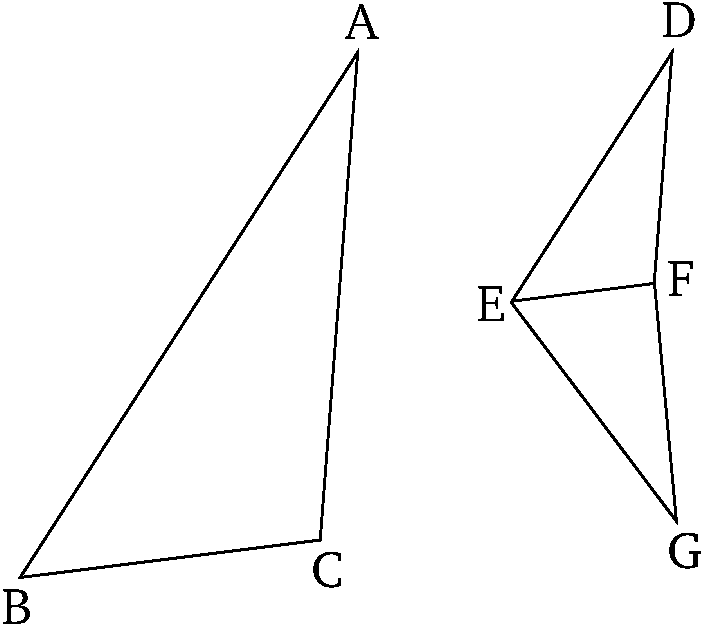
\includegraphics{Book06/fig05e.pdf}}

Thus, triangle $ABC$ is equiangular to [triangle] $EGF$. Thus, for triangles
$ABC$ and $EGF$, the sides about the equal angles are proportional, and
(those) sides subtending equal angles correspond [Prop.~6.4]. Thus, as $AB$ is to $BC$, [so]
$GE$ (is) to $EF$. But, as $AB$ (is) to $BC$, so, it was assumed, (is) $DE$  to
$EF$. Thus, as $DE$ (is) to $EF$, so $GE$ (is) to $EF$ [Prop.~5.11]. Thus, $DE$ and $GE$ each have the
same ratio to $EF$. Thus, $DE$ is equal to $GE$ [Prop.~5.9]. So, for the same (reasons), 
$DF$ is also equal to $GF$. Therefore, since $DE$ is equal to $EG$, and $EF$ (is)
common, the two (sides) $DE$, $EF$ are equal to the two (sides)
$GE$, $EF$ (respectively). And base $DF$ [is] equal to base $FG$. Thus, angle $DEF$
is equal to angle $GEF$  [Prop.~1.8],  and triangle $DEF$ (is) equal to triangle $GEF$,  and the remaining angles (are) equal to the remaining
angles which the equal sides subtend  [Prop.~1.4]. Thus,
angle $DFE$ is also equal to $GFE$, and (angle) $EDF$ to $EGF$. And since 
(angle) $FED$ is equal to $GEF$, and (angle) $GEF$ to $ABC$, angle $ABC$ is
thus also equal to $DEF$. So, for the same (reasons), (angle) $ACB$ is
also equal to $DFE$, and, further, the (angle) at $A$ to the (angle) at $D$.
Thus, triangle $ABC$ is equiangular to triangle $DEF$.

Thus,  if two triangles have proportional sides, (then) the
triangles will be equiangular, and will have the angles which  corresponding sides
subtend  equal. (Which is) the very thing it was required to show.}
\end{Parallel}

%%%%%%
% Prop 6.6
%%%%%%
\pdfbookmark[1]{Proposition 6.6}{pdf6.6}
\begin{Parallel}{}{} 
\ParallelLText{
\begin{center}
{\large \ggn{6}.}
\end{center}\vspace*{-7pt}

\gr{Ἐὰν δύο τρίγωνα μίαν γωνίαν μιᾶ| γωνίᾳ >ίσην >έθῃ, περὶ
δὲ τὰξ  >ίσαξ γωνίαξ τὰξ πλευρὰξ ἀνάλογον, ἰσογώνια
>έσται τὰ τρίγωνα καὶ >ίσαξ <έχει τὰξ γωνίαξ, ὑφ> <ὰξ αἱ
ὁμόλογοι πλευραὶ ὑποτείνουσιν.}

\gr{>'Εστω δύο τρίγωνα τὰ ΑΒΓ, ΔΕΖ μίαν γωνίαν τὴν ὑπὸ ΒΑΓ
μιᾶ| γωνίᾳ τῆ| ὑπὸ ΕΔΖ >ίσην >έθοντα, περὶ δὲ τὰξ >ίσαξ
γωνίαξ τὰξ πλευρὰξ ἀνάλογον, ὡξ τὴν ΒΑ πρὸξ τὴν ΑΓ, ο<ύτωξ
τὴν ΕΔ πρὸξ τὴν ΔΖ; λέγω, <ότι ἰσογώνιόν ἐστι τὸ ΑΒΓ τρίγωνον
τῶ| ΔΕΖ τριγώνῳ καὶ >ίσην <έχει τὴν ὑπὸ ΑΒΓ γωνίαν
τῆ| ὑπὸ ΔΕΖ, τὴν δὲ ὑπὸ ΑΓΒ τῆ| ὑπὸ ΔΖΕ.}

% Removed epsf size command
\centerline{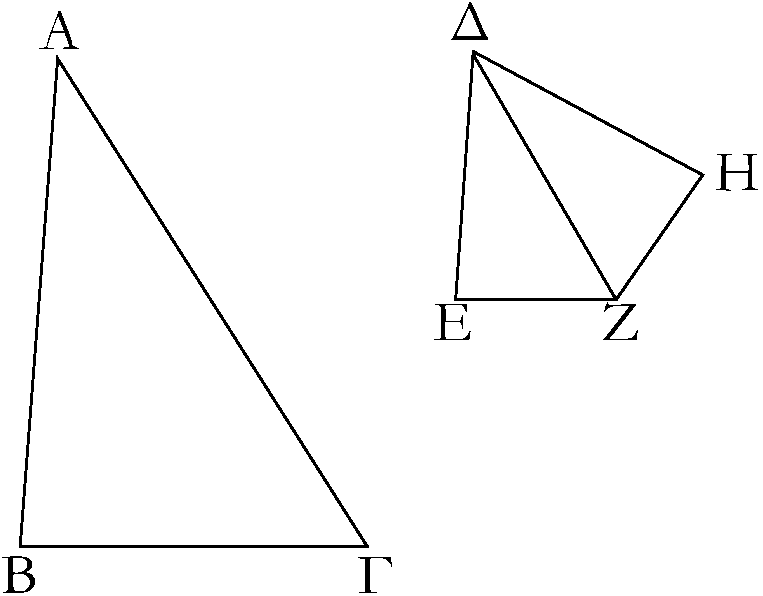
\includegraphics{Book06/fig06g.pdf}}

\gr{Συνεστάτω γὰρ πρὸξ τῆ| ΔΖ εὐθείᾳ καὶ τοῖξ πρὸξ α\kern -.7pt  ὐτῆ| σημείοιξ
τοῖξ Δ, Ζ ὁποτέρᾳ μὲν τῶν ὑπὸ ΒΑΓ, ΕΔΖ >ίση ἡ ὑπὸ 
ΖΔΗ, τῆ| δὲ ὑπὸ ΑΓΒ >ίση ἡ ὑπὸ ΔΖΗ; λοιπὴ >άρα ἡ πρὸξ 
τῶ| Β γωνία λοιπῆ| τῆ| πρὸξ τῶ| Η >ίση ἐστίν.}

\gr{Ἰσογώνιον >άρα ἐστὶ τὸ ΑΒΓ τρίγωνον τῶ| ΔΗΖ τριγώνῳ. ἀνάλογον >άρα ἐστὶν ὡξ ἡ ΒΑ πρὸξ τὴν ΑΓ, ο<ύτωξ ἡ ΗΔ πρὸξ τὴν ΔΖ.
ὑπόκειται δὲ καὶ ὡξ ἡ ΒΑ πρὸξ τὴν ΑΓ, ο<ύτωξ ἡ ΕΔ πρὸξ
τὴν ΔΖ; καὶ ὡξ >άρα ἡ ΕΔ πρὸξ τὴν ΔΖ, ο<ύτωξ  ἡ ΗΔ πρὸξ
τὴν ΔΖ. >ίση >άρα ἡ ΕΔ τῆ| ΔΗ; καὶ κοινὴ ἡ ΔΖ;
δύο δὴ αἱ ΕΔ, ΔΖ δυσὶ ταῖξ ΗΔ, ΔΖ >ίσαξ εἰσίν; καὶ γωνία
ἡ ὑπὸ ΕΔΖ γωνίᾳ τῆ| ὑπὸ ΗΔΖ [ἐστιν]
>ίση; βάσιξ >άρα ἡ ΕΖ βάσει τῆ| ΗΖ ἐστιν >ίση, καὶ τὸ ΔΕΖ τρίγωνον
τῶ| ΗΔΖ τριγώνῳ >ίσον ἐστίν, καὶ αἱ λοιπαὶ γωνίαι ταῖξ λοιπαῖξ
γωνίαιξ >ίσαξ >έσονται, ὐφ> <ὰξ >ίσαξ πλευραὶ ὑποτείνουσιν.
>ίση >άρα ἐστὶν ἡ μὲν ὑπὸ ΔΖΗ τῆ| ὑπὸ ΔΖΕ, ἡ δὲ ὑπὸ
ΔΗΖ τῆ| ὑπὸ ΔΕΖ. ἀλλ> ἡ ὑπὸ ΔΖΗ τῆ| ὑπὸ
ΑΓΒ ἐστιν >ίση; καὶ ἡ ὑπὸ ΑΓΒ >άρα τῆ| ὑπὸ ΔΖΕ ἐστιν
>ίση. ὑπόκειται δὲ καὶ ἡ ὑπὸ ΒΑΓ τῆ| ὑπὸ ΕΔΖ >ίση;
καὶ λοιπὴ >άρα ἡ πρὸξ τῶ| Β λοιπῆ| τῆ| πρὸξ τῶ| Ε >ίση
ἐστίν; ἰσογώνιον >άρα ἐστὶ τὸ ΑΒΓ τρίγωνον τῶ| ΔΕΖ
τριγώνῳ.}

\gr{Ἐὰν >άρα δύο τρίγωνα μίαν γωνίαν μιᾶ| γωνίᾳ >ίσην >έθῃ, περὶ
δὲ τὰξ  >ίσαξ γωνίαξ τὰξ πλευρὰξ ἀνάλογον, ἰσογώνια
>έσται τὰ τρίγωνα καὶ >ίσαξ <έχει τὰξ γωνίαξ, ὑφ> <ὰξ αἱ
ὁμόλογοι πλευραὶ ὑποτείνουσιν; <όπερ >έδει δεῖχαι.}}

\ParallelRText{
\begin{center}
{\large Proposition 6}
\end{center}

If two triangles have one angle equal to one angle,
and the sides about the equal angles proportional, (then) the triangles will
be equiangular, and will have the angles which corresponding sides subtend equal.

Let $ABC$ and $DEF$ be two triangles having one angle, $BAC$, equal to
one angle, $EDF$ (respectively), and the sides about the equal angles proportional,
(so that) as $BA$ (is) to $AC$, so $ED$ (is) to $DF$. I say that triangle $ABC$ is
equiangular to triangle $DEF$, and will have angle $ABC$ equal to
$DEF$, and (angle) $ACB$ to $DFE$.

% Removed epsf size command
\centerline{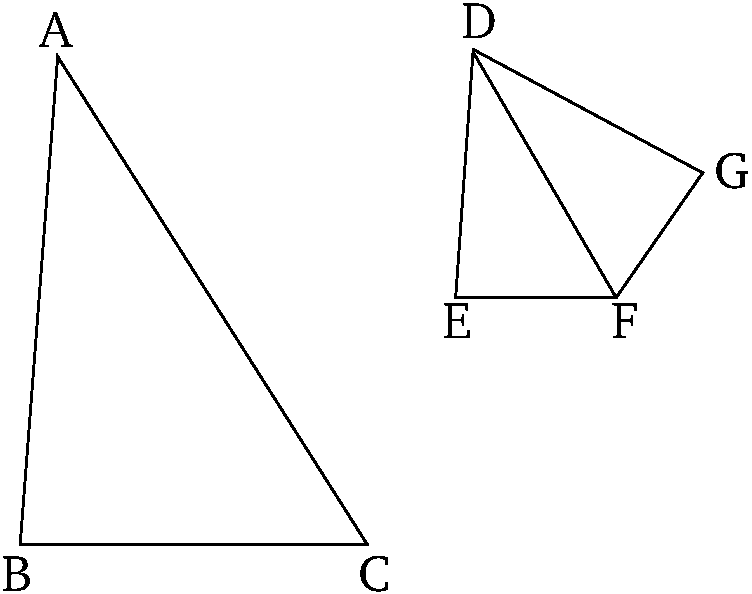
\includegraphics{Book06/fig06e.pdf}}

For let (angle) $FDG$, equal to each of $BAC$ and $EDF$, and (angle) $DFG$, equal to $ACB$, be constructed on the
straight-line $AF$ at the points $D$ and $F$ on it (respectively)   [Prop.~1.23]. Thus, the remaining angle at $B$
is equal to the remaining angle at $G$  [Prop.~1.32].

Thus, triangle $ABC$ is equiangular to triangle $DGF$. Thus, proportionally,
as $BA$ (is) to $AC$, so $GD$ (is) to $DF$ [Prop.~6.4].  And it was also assumed that as $BA$
(is) to $AC$, so $ED$ (is) to $DF$. And, thus, as $ED$ (is) to $DF$, so $GD$ (is) to $DF$ [Prop.~5.11]. Thus, $ED$ (is) equal to $DG$ [Prop.~5.9]. And $DF$ (is) common. So, the two
(sides) $ED$, $DF$ are equal to the two (sides) $GD$, $DF$ (respectively). And 
angle $EDF$ [is] equal to  angle $GDF$. Thus,  base $EF$ is equal to
base $GF$, and triangle $DEF$ is equal to triangle $GDF$, and the remaining
angles will be equal to the remaining angles which the equal sides subtend
 [Prop.~1.4]. Thus, (angle) $DFG$ is equal to $DFE$, and (angle) $DGF$ to
$DEF$. But, (angle) $DFG$ is equal to $ACB$. Thus, (angle) $ACB$ is also equal
to $DFE$. And  (angle) $BAC$ was also assumed (to be) equal to $EDF$. 
Thus, the remaining (angle) at $B$ is equal to the remaining (angle) at $E$  [Prop.~1.32]. Thus, triangle $ABC$ is equiangular to triangle $DEF$.

Thus, if two triangles have one angle equal to one angle,
and the sides about the equal angles proportional, (then) the triangles will
be equiangular, and will have the angles which corresponding sides subtend equal. (Which is) the very thing it was required to show.}
\end{Parallel}

%%%%%%
% Prop 6.7
%%%%%%
\pdfbookmark[1]{Proposition 6.7}{pdf6.7}
\begin{Parallel}{}{} 
\ParallelLText{
\begin{center}
{\large \ggn{7}.}
\end{center}\vspace*{-7pt}

\gr{Ἐὰν δύο τρίγωνα μίαν γωνίαν μιᾶ| γωνίᾳ >ίσην >έθῃ, περὶ
δὲ >άλλαξ γωνίαξ τὰξ πλευρὰξ ἀνάλογον, τῶν δὲ λοιπῶν ἑκατέραν
<άμα >ήτοι ἐλάσσονα >ὴ μ\kern -.7pt  ὴ ἐλάσσονα ὀρθῆξ, ἰσογώνια >έσται
τὰ τρίγωνα καὶ >ίσαξ <έχει τὰξ γωνίαξ, 
περὶ <ὰξ ἀνάλογόν εἰσιν αἱ πλευραί.}

\gr{>'Εστω δύο τρίγωνα τὰ ΑΒΓ, ΔΕΖ μίαν γωνίαν μιᾶ| γωνίᾳ >ίσην
>έθοντα τὴν ὑπὸ ΒΑΓ τῆ| ὑπὸ ΕΔΖ, περὶ δὲ >άλλαξ γωνίαξ
τὰξ ὑπὸ ΑΒΓ, ΔΕΖ τὰξ πλευρὰξ ἀνάλογον, ὡξ τὴν ΑΒ πρὸξ τὴν
ΒΓ, ο<ύτωξ τὴν ΔΕ πρὸξ τὴν ΕΖ, τῶν δὲ λοιπῶν τῶν πρὸξ τοῖξ
Γ, Ζ πρότερον ἑκατέραν <άμα ἐλάσσονα ὀρθῆξ; λέγω, <ότι
ἰσογώνιόν ἐστι τὸ ΑΒΓ τρίγωνον τῶ| ΔΕΖ τριγώνῳ, καὶ >ίση
>έσται ἡ ὑπὸ ΑΒΓ γωνία τῆ| ὑπὸ ΔΕΖ, καὶ λοιπὴ δηλονότι
ἡ πρὸξ τῶ| Γ λοιπῆ| τῆ| πρὸξ τῶ| Ζ >ίση.}\\

% Removed epsf size command
\centerline{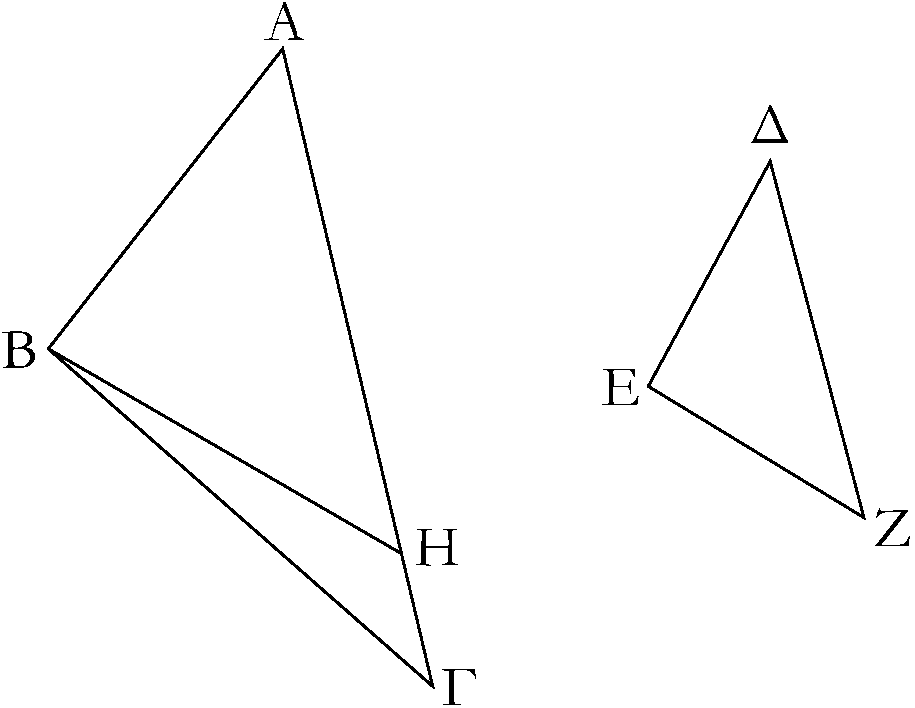
\includegraphics{Book06/fig07g.pdf}}

\gr{Εἰ γὰρ >άνισόξ ἐστιν ἡ ὑπὸ ΑΒΓ γωνία τῆ| ὑπὸ
ΔΕΖ, μία α\kern -.7pt  ὐτῶν μείζων ἐστίν. >έστω μείζων ἡ ὑπὸ
ΑΒΓ. καὶ συνεστάτω πρὸξ τῆ| ΑΒ εὐθείᾳ καὶ τῶ|
πρὸξ α\kern -.7pt  ὐτῆ| σημείῳ τῶ| Β τῆ| ὑπὸ ΔΕΖ γωνίᾳ >ίση ἡ
ὑπὸ ΑΒΗ.}

\gr{Καὶ ἐπεὶ >ίση ἐστὶν ἡ μὲν Α γωνία τῆ| Δ, ἡ δὲ ὑπὸ ΑΒΗ τῆ|
ὑπὸ ΔΕΖ, λοιπὴ >άρα ἡ ὑπὸ ΑΗΒ λοιπῆ| τῆ| ὑπὸ ΔΖΕ ἐστιν
>ίση. ἰσογώνιον >άρα ἐστὶ τὸ ΑΒΗ τρίγωνον τῶ| ΔΕΖ τριγώνῳ.
>έστιν >άρα ὡξ ἡ ΑΒ πρὸξ τὴν ΒΗ, ο<ύτωξ ἡ ΔΕ πρὸξ τὴν ΕΖ.
ὡξ δὲ ἡ ΔΕ πρὸξ τὴν ΕΖ, [ο<ύτωξ] ὑπόκειται ἡ ΑΒ πρὸξ τὴν
ΒΓ; ἡ ΑΒ >άρα πρὸξ ἑκατέραν τῶν ΒΓ, ΒΗ τὸν α\kern -.7pt  ὐτὸν >έθει
λόγον; >ίση >άρα ἡ ΒΓ τῆ| ΒΗ. <ώστε καὶ γωνία ἡ πρὸξ τῶ| Γ
γωνίᾳ τῆ| ὑπὸ ΒΗΓ ἐστιν >ίση. ἐλάττων δὲ ὀρθῆξ ὑπόκειται
ἡ πρὸξ τῶ| Γ;
ἐλάττων >άρα ἐστὶν ὀρθῆξ
καὶ ὑπὸ ΒΗΓ;  <ώστε ἡ ἐφεχῆξ α\kern -.7pt  ὐτῆ| γωνία ἡ ὑπὸ ΑΗΒ
μείζων ἐστὶν ὀρθῆξ. καὶ ἐδείθθη >ίση ο>ῦσα τῆ| πρὸξ τῶ|
Ζ; καὶ ἡ πρὸξ τῶ| Ζ >άρα μείζων ἐστὶν ὀρθῆξ. ὑπόκειται
δὲ ἐλάσσων ὀρθῆξ; <όπερ ἐστὶν >άτοπον. οὐκ >άρα >άνισόξ
ἐστιν ἡ ὑπὸ ΑΒΓ γωνία τῆ| ὑπὸ ΔΕΖ; >ίση >άρα. >έστι δὲ καὶ ἡ πρὸξ τῶ| Α >ίση τῆ| πρὸξ τῶ| Δ;
καὶ λοιπὴ >άρα ἡ πρὸξ τῶ| Γ λοιπῆ| τῆ| πρὸξ τῶ| Ζ >ίση ἐστίν.
ἰσογώνιον >άρα ἐστὶ τὸ ΑΒΓ τρίγωνον τῶ| ΔΕΖ τριγώνῳ.}

\gr{Ἀλλὰ δὴ πάλιν ὑποκείσθω ἑκατέρα τῶν πρὸξ τοῖξ Γ, Ζ μ\kern -.7pt  ὴ
ἐλάσσων ὀρθῆξ; λέγω πάλιν, <ότι καὶ ο<ύτωξ ἐστὶν ἰσογώνιον
τὸ ΑΒΓ τρίγωνον τῶ| ΔΕΖ τριγώνῳ.}

\gr{Τῶν γὰρ α\kern -.7pt  ὐτῶν κατασκευασθέντων ὁμοίωξ δείχομεν, <ότι
>ίση ἐστὶν ἡ ΒΓ τῆ| ΒΗ; <ώστε καὶ γωνία ἡ πρὸξ τῶ| Γ τῆ| ὑπὸ
ΒΗΓ >ίση ἐστίν. οὐκ ἐλάττων δὲ ὀρθῆξ ἡ πρὸξ τῶ| Γ; οὐκ
ἐλάττων >άρα ὀρθῆξ οὐδὲ ἡ ὑπὸ ΒΗΓ. τριγώνου δὴ τοῦ
ΒΗΓ αἱ δύο γωνίαι δύο ὀρθῶν ο>ύκ εἰσιν ἐλάττονεξ; <όπερ
ἐστὶν ἀδύνατον. οὐκ >άρα πάλιν >άνισόξ ἐστιν ἡ ὑπὸ
ΑΒΓ γωνία τῆ| ὑπὸ ΔΕΖ; >ίση >άρα. >έστι δὲ καὶ ἡ πρὸξ
τῶ| Α τῆ| πρὸξ τῶ| Δ >ίση; λοιπὴ >άρα ἡ πρὸξ τῶ| Γ λοιπῆ|
τῆ| πρὸξ τῶ| Ζ >ίση ἐστίν. ἰσογώνιον >άρα ἐστὶ τὸ ΑΒΓ τρίγωνον
τῶ| ΔΕΖ τριγώνῳ.}

\gr{Ἐὰν >άρα δύο τρίγωνα μίαν γωνίαν μιᾶ| γωνίᾳ >ίσην >έθῃ, περὶ
δὲ >άλλαξ γωνίαξ τὰξ πλευρὰξ ἀνάλογον, τῶν δὲ λοιπῶν ἑκατέραν
<άμα  ἐλάττονα >ὴ μ\kern -.7pt  ὴ ἐλάττονα ὀρθῆξ, ἰσογώνια >έσται
τὰ τρίγωνα καὶ >ίσαξ <έχει τὰξ γωνίαξ,
περὶ <ὰξ ἀνάλογόν εἰσιν αἱ πλευραί; <όπερ >έδει δεῖχαι.}}

\ParallelRText{
\begin{center}
{\large Proposition 7}
\end{center}

If two triangles have one angle equal to one angle,
and the sides about  other angles proportional, and the remaining angles
either both less than, or both not less than, right-angles, (then) the triangles will
be equiangular, and will have the angles about which the sides are proportional equal.

Let $ABC$ and $DEF$ be two triangles having one angle, $BAC$,  equal to one angle, $EDF$ (respectively), and  the sides about (some) other angles, $ABC$ and
$DEF$ (respectively), proportional, (so that) as $AB$ (is) to $BC$, so
$DE$ (is) to $EF$, and the remaining (angles) at $C$ and $F$, first of all, both
less than right-angles. I say that triangle $ABC$ is equiangular to triangle
$DEF$, and (that) angle $ABC$ will be equal to $DEF$, and (that) the remaining  (angle) at $C$
(will be) manifestly equal to the remaining (angle) at $F$.

% Removed epsf size command
\centerline{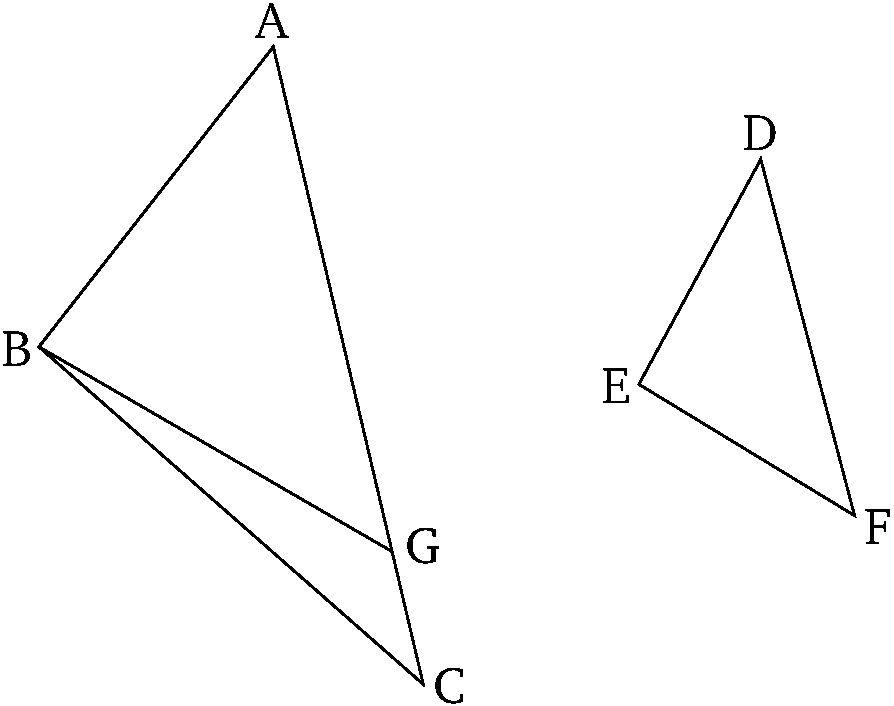
\includegraphics{Book06/fig07e.pdf}}

For if angle $ABC$ is not equal to (angle) $DEF$, (then) one of them is greater.
Let $ABC$ be greater. And let (angle) $ABG$, equal to (angle) $DEF$, be constructed on the straight-line $AB$  at the point $B$  on it [Prop.~1.23].

And since angle $A$ is equal to (angle) $D$, and (angle) $ABG$ to $DEF$, the remaining
(angle) $AGB$ is thus equal to the remaining (angle) $DFE$  [Prop.~1.32].
Thus, triangle $ABG$ is equiangular to triangle $DEF$. Thus, as $AB$ is to
$BG$, so $DE$ (is) to $EF$ [Prop.~6.4]. 
And as $DE$ (is) to $EF$, [so] it was assumed (is) $AB$ to $BC$. Thus, $AB$ has the
same ratio to each of $BC$ and $BG$ [Prop.~5.11].
Thus, $BC$ (is) equal to $BG$ [Prop.~5.9].
And, hence, the angle at $C$ is equal to angle $BGC$  [Prop.~1.5].
And the angle at $C$ was assumed (to be) less than a right-angle.
Thus, (angle) $BGC$ is also less than a right-angle. Hence, the adjacent
angle to it, $AGB$, is greater than a right-angle [Prop.~1.13].
And ($AGB$) was shown to be equal to the (angle) at $F$. Thus, the (angle)
at $F$ is also greater than a right-angle. But it was assumed (to be)
less than a right-angle. The very thing is absurd. Thus, angle $ABC$ is
not unequal to (angle) $DEF$. Thus, (it is) equal. And the (angle) at $A$ is also
equal to the (angle) at $D$. And thus the remaining (angle) at $C$ is equal
to the remaining (angle) at $F$  [Prop.~1.32]. Thus, triangle $ABC$
is equiangular to triangle $DEF$.

But, again, let each of the (angles) at $C$ and $F$ be assumed  (to be) not
less than a right-angle. I say, again, that triangle $ABC$
is equiangular to triangle $DEF$ in this case also.

For, with the same construction, we can similarly show that $BC$ is equal to $BG$.
Hence, also, the angle at $C$ is equal to (angle) $BGC$. And  the (angle) at $C$ (is)
not less than a right-angle. Thus, $BGC$ (is) not less than a right-angle
either. So, in triangle $BGC$ the (sum of) two angles is not less than two
right-angles. The very thing is impossible [Prop.~1.17]. Thus, again,
angle $ABC$ is not unequal to $DEF$. Thus, (it is) equal.  And the (angle) at $A$
is also equal to the (angle) at $D$. Thus, the remaining (angle) at $C$ is equal
to the remaining (angle) at $F$ [Prop.~1.32]. Thus, triangle $ABC$ is equiangular to triangle $DEF$.

Thus, if two triangles have one angle equal to one angle,
and the sides about  other angles proportional, and the remaining angles
both less than, or both not less than, right-angles, (then) the triangles will
be equiangular, and will have the angles about which the sides (are) proportional equal. (Which is) the very thing it was required to show.}
\end{Parallel}

%%%%%%
% Prop 6.8
%%%%%%
\pdfbookmark[1]{Proposition 6.8}{pdf6.8}
\begin{Parallel}{}{} 
\ParallelLText{
\begin{center}
{\large \ggn{8}.}
\end{center}\vspace*{-7pt}

\gr{Ἐὰν ἐν ὀρθογωνίῳ τριγώνῳ ἀπό τῆξ ὀρθῆξ γωνίαξ ἐπὶ
τὴν βάσιν κάθετοξ ἀθθῆ|, τὰ πρὸξ τῆ| καθέτῳ τρίγωνα <όμοιά
ἐστι τῶ| τε <όλῳ καὶ ἀλλήλοιξ.}

\gr{>'Εστω τρίγωνον ὀρθογώνιον τὸ ΑΒΓ ὀρθὴν >έθον τὴν ὑπὸ
ΒΑΓ γωνίαν, καὶ >ήθθω ἀπὸ τοῦ Α ἐπὶ τὴν ΒΓ κάθετοξ
ἡ ΑΔ; λέγω, <ότι <όμοιόν ἐστιν ἑκάτερον τῶν ΑΒΔ, ΑΔΓ 
τριγώνων <όλῳ τῶ| ΑΒΓ καὶ >έτι ἀλλήλοιξ.}\\

% Removed epsf size command
\centerline{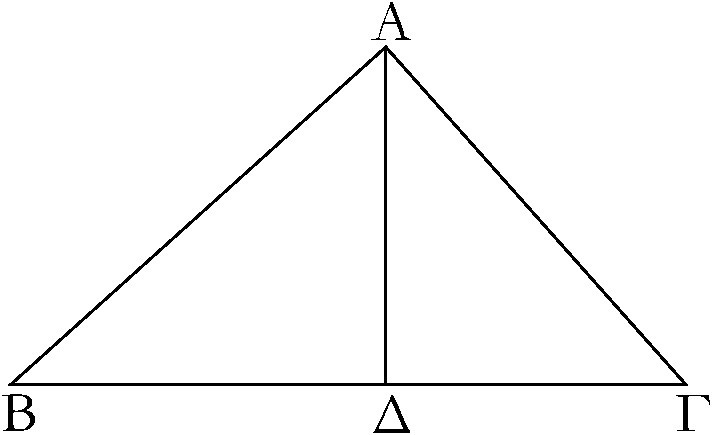
\includegraphics{Book06/fig08g.pdf}}

\gr{Ἐπεὶ γὰρ >ίση ἐστὶν ἡ ὑπὸ ΒΑΓ τῆ| ὑπὸ ΑΔΒ;
ὀρθὴ γὰρ ἑκατέρα; καὶ κοινὴ τῶν δύο τριγώνων τοῦ τε
ΑΒΓ καὶ τοῦ ΑΒΔ ἡ πρὸξ τῶ| Β, λοιπὴ >άρα ἡ ὑπὸ
ΑΓΒ λοιπῆ| τῆ| ὑπὸ ΒΑΔ ἐστιν >ίση; ἰσογώνιον >άρα ἐστὶ
τὸ ΑΒΓ τρίγωνον τῶ| ΑΒΔ τριγώνῳ. >έστιν >άρα ὡξ ἡ ΒΓ ὑποτείνουσα τὴν ὀρθὴν τοῦ ΑΒΓ τριγώνου πρὸξ τὴν ΒΑ ὑποτείνουσαν
τὴν ὀρθὴν  τοῦ ΑΒΔ τριγώνου, ο<ύτωξ α\kern -.7pt  ὐτὴ ἡ ΑΒ ὑποτείνουσα τὴν
πρὸξ τῶ| Γ γωνίαν τοῦ ΑΒΓ τριγώνου πρὸξ τὴν ΒΔ ὑποτείνουσαν
τὴν >ίσην τὴν ὑπὸ ΒΑΔ τοῦ ΑΒΔ τριγώνου, καὶ >έτι ἡ ΑΓ
πρὸξ τὴν ΑΔ ὑποτείνουσαν τὴν πρὸξ τῶ| Β γωνίαν
κοινὴν τῶν δύο τριγώνων. τὸ ΑΒΓ >άρα τρίγωνον τῶ| ΑΒΔ 
τριγώνῳ ἰσογώνιόν τέ ἐστι καὶ τὰξ περὶ τὰξ >ίσαξ γωνίαξ
πλευρὰξ ἀνάλογον >έθει. <όμοιον >άμα [ἐστὶ]
τὸ ΑΒΓ τρίγωνον τῶ| ΑΒΔ τριγώνῳ. ὁμοίωξ δὴ δείχομεν,
<ότι καὶ τῶ| ΑΔΓ τριγώνῳ <όμοιόν ἐστι τὸ ΑΒΓ τρίγωνον;
ἑκάτερον >άρα τῶν ΑΒΔ, ΑΔΓ [τριγώνων] <όμοιόν ἐστιν <όλῳ
τῶ| ΑΒΓ.}

\gr{Λέγω δή, <ότι καὶ ἀλλήλοιξ ἐστὶν <όμοια τὰ ΑΒΔ, ΑΔΓ τρίγωνα.}

\gr{Ἐπεὶ γὰρ ὀρθὴ ἡ ὑπὸ ΒΔΑ ὀρθῆ| τῆ| ὑπὸ ΑΔΓ
ἐστιν >ίση, ἀλλὰ μ\kern -.7pt  ὴν καὶ ἡ ὑπὸ ΒΑΔ τῆ| πρὸξ τῶ| Γ
ἐδείθθη >ίση, καὶ λοιπὴ >άρα ἡ πρὸξ τῶ| Β λοιπῆ| τῆ| ὑπὸ ΔΑΓ
ἐστιν >ίση; ἰσογώνιον >άρα ἐστὶ τὸ ΑΒΔ τρίγωνον τῶ| ΑΔΓ
τριγώνῳ. >έστιν >άρα ὡξ ἡ ΒΔ  τοῦ ΑΒΔ τριγώνου ὑποτείνουσα
τὴν ὑπὸ ΒΑΔ πρὸξ τὴν ΔΑ τοῦ ΑΔΓ τριγώνου ὑποτείνουσαν
τὴν πρὸξ τῶ| Γ  >ίσην τῆ| ὑπὸ ΒΑΔ, ο<ύτωξ α\kern -.7pt  ὐτὴ ἡ ΑΔ
τοῦ ΑΒΔ τριγώνου ὑποτείνουσα τὴν πρὸξ τῶ| Β γωνίαν
πρὸξ τὴν ΔΓ ὑποτείνουσαν τὴν ὑπὸ ΔΑΓ τοῦ ΑΔΓ τριγώνου
>ίσην τῆ| πρὸξ τῶ| Β, καὶ >έτι ἡ ΒΑ πρὸξ 
τὴν ΑΓ ὑποτείνουσαι τὰξ ὀρθάξ; <όμοιον >άρα ἐστὶ τὸ
ΑΒΔ τρίγωνον τῶ| ΑΔΓ τριγώνῳ.}

\gr{Ἐὰν >άρα ἐν ὀρθογωνίῳ τριγώνῳ ἀπὸ τῆξ ὀρθῆξ γωνίαξ ἐπὶ
τὴν βάσιν κάθετοξ ἀθθῆ|, τὰ πρὸξ τῆ| καθέτῳ τρίγωνα <όμοιά
ἐστι τῶ| τε <όλῳ καὶ ἀλλήλοιξ [<όπερ >έδει δεῖχαι].}\\~\\~\\~\\

\begin{center}
{\large \gr{Πόρισμα}.}
\end{center}\vspace*{-7pt}

\gr{Ἐκ δὴ τούτου φανερόν, <ότι ἒαν ἐν ὀρθογωνίῳ
τριγώνῳ ἀπὸ τῆξ ὀρθῆξ γωνάιξ ἐπὶ τὴν βάσιξ
κάθετοξ ἀθθῆ|, ἡ ἀθθεῖσα τῶν τῆξ βάσεωξ τμ\kern -.7pt  ημάτων
μέση ἀνάλογόν ἐστιν; <όπερ >έδει δεῖχαι.}}

\ParallelRText{
\begin{center}
{\large Proposition 8}
\end{center}

If, in a right-angled triangle, a (straight-line) is drawn from the right-angle perpendicular
to the base,  (then) the triangles around the perpendicular are similar to
the whole (triangle), and to one another.

Let $ABC$ be a right-angled triangle having the angle $BAC$ a right-angle, 
and let $AD$ be drawn from $A$, perpendicular to $BC$  
[Prop.~1.12].  I say that
triangles $ABD$ and $ADC$ are each similar to the whole (triangle) $ABC$ and, further, to one another.

% Removed epsf size command
\centerline{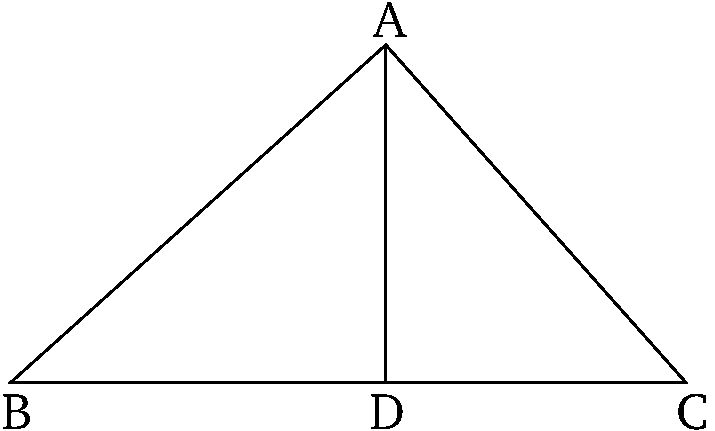
\includegraphics{Book06/fig08e.pdf}}

For since (angle) $BAC$ is equal to $ADB$---for each (are) right-angles---and the (angle) at $B$ (is) common to the two triangles $ABC$ and
$ABD$, the remaining (angle) $ACB$ is thus equal to the remaining (angle)
$BAD$  [Prop.~1.32]. Thus, triangle $ABC$ is equiangular to triangle $ABD$. 
Thus, as $BC$, subtending  the right-angle in triangle $ABC$, is to
$BA$, subtending the right-angle in triangle $ABD$, so the
same $AB$, subtending the angle at $C$ in triangle $ABC$, (is) to
$BD$, subtending the equal (angle) $BAD$ in triangle $ABD$,
and, further, (so is) $AC$ to $AD$, (both) subtending the angle at $B$ common to
the two triangles [Prop.~6.4].
Thus, triangle $ABC$ is equiangular to triangle $ABD$, and has the
sides about the equal angles proportional. Thus, triangle $ABC$
[is] similar to triangle $ABD$ [Def.~6.1].
So, similarly, we can show that triangle $ABC$ is also  similar to triangle
$ADC$. Thus, [triangles] $ABD$ and $ADC$ are each similar to the whole
 (triangle) $ABC$.
 
 So I say that triangles $ABD$ and $ADC$ are also similar to one another.
 
 For since the right-angle $BDA$ is equal to the right-angle $ADC$, and, indeed,
 (angle) $BAD$ was also shown (to be) equal to the (angle) at $C$, thus the
 remaining (angle) at $B$ is also equal to the remaining (angle) $DAC$ 
 [Prop.~1.32].
  Thus, triangle $ABD$ is equiangular to triangle $ADC$.
 Thus, as $BD$, subtending (angle) $BAD$ in triangle $ABD$, is to
 $DA$, subtending the (angle) at $C$ in triangle $ADC$, (which is) equal to (angle) $BAD$, so (is) the
 same $AD$, subtending the angle at $B$ in triangle $ABD$, to $DC$, subtending
 (angle) $DAC$ in triangle $ADC$, (which is) equal to the (angle) at $B$,
 and, further, (so is) $BA$ to $AC$, (each) subtending  right-angles [Prop.~6.4]. Thus, triangle $ABD$ is similar to
 triangle $ADC$  [Def.~6.1].
 
 Thus,  if, in a right-angled triangle, a (straight-line) is drawn from the right-angle perpendicular
to the base,  (then) the triangles around the perpendicular are similar to
the whole (triangle), and to one another. [(Which is) the very thing it
was required to show.]\\

\begin{center}
{\large Corollary}
\end{center}\vspace*{-7pt}

So (it is) clear, from this, that if, in a right-angled triangle, a
(straight-line) is drawn from the right-angle perpendicular to the base, (then) the (straight-line so)
drawn is in mean proportion to the pieces of the base.$^\dag$ (Which
is) the very thing it was required to show.}
\end{Parallel}
{\footnotesize \noindent$^\dag$ In other words, the perpendicular is the geometric mean of the pieces.} 

%%%%%%
% Prop 6.9
%%%%%%
\pdfbookmark[1]{Proposition 6.9}{pdf6.9}
\begin{Parallel}{}{} 
\ParallelLText{
\begin{center}
{\large \ggn{9}.}
\end{center}\vspace*{-7pt}

\gr{Τῆξ δοθείσηξ εὐθείαξ τὸ προσταθθὲν μέροξ ἀφελεῖν.}

\gr{>'Εστω ἡ δοθεῖσα εὐθεῖα ἡ ΑΒ; δεῖ δὴ τῆξ ΑΒ τὸ
προσταθθὲν μέροξ ἀφελεῖν.}

% Removed epsf size command
\centerline{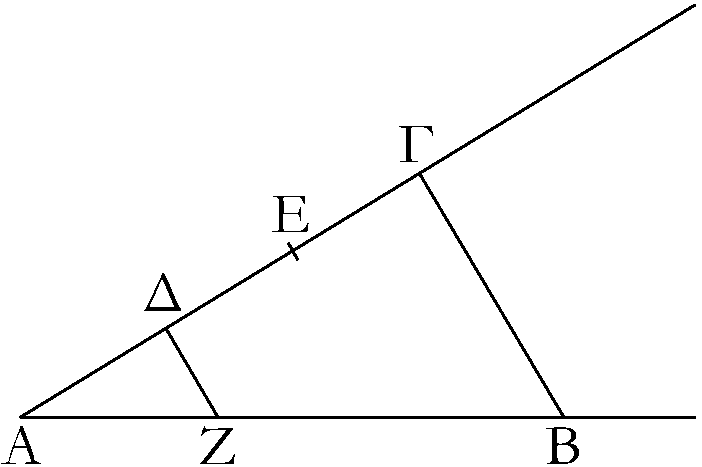
\includegraphics{Book06/fig09g.pdf}}

\gr{Ἐπιτετάθθω δὴ τὸ τρίτον. [καὶ] διήθθω τιξ ἀπὸ τοῦ Α εὐθεῖα
ἡ ΑΓ γωνίαν περιέθουσα μετὰ τῆξ ΑΒ τυθοῦσαν; καὶ εἰλήφθω
τυθὸν σημεῖον ἐπὶ τῆξ ΑΓ τὸ Δ, καὶ κείσθωσαν τῆ| ΑΔ
>ίσαι αἱ ΔΕ, ΕΓ. καὶ ἐπεζεύθθω ἡ ΒΓ, καὶ διὰ τοῦ Δ παράλληλοξ
α\kern -.7pt  ὐτῆ| >ήθθω ἡ ΔΖ.}

\gr{Ἐπεὶ ο>ῦν τριγώνου τοῦ ΑΒΓ παρὰ μίαν τῶν πλευρῶν
τὴν ΒΓ >ῆκται ἡ ΖΔ, ἀνάλογον >άρα ἐστὶν ὡξ ἡ ΓΔ πρὸξ
τὴν ΔΑ, ο<ύτωξ ἡ ΒΖ πρὸξ τὴν ΖΑ. διπλῆ δὲ ἡ ΓΔ τῆξ
ΔΑ; διπλῆ >άρα καὶ ἡ ΒΖ τῆξ ΖΑ; τριπλῆ >άρα ἡ ΒΑ τῆξ ΑΖ.}

\gr{Τῆξ >άρα δοθείσηξ εὐθείαξ τῆξ ΑΒ τὸ ἐπιταθθὲν τρίτον μέροξ
ἀφή|ρηται τὸ ΑΖ; <όπερ >έδει ποιῆσαι.}}

\ParallelRText{
\begin{center}
{\large Proposition 9}
\end{center}

To cut off a prescribed part from a given straight-line.

Let $AB$ be the given straight-line. So it is required to cut off a prescribed
part from $AB$.

% Removed epsf size command
\centerline{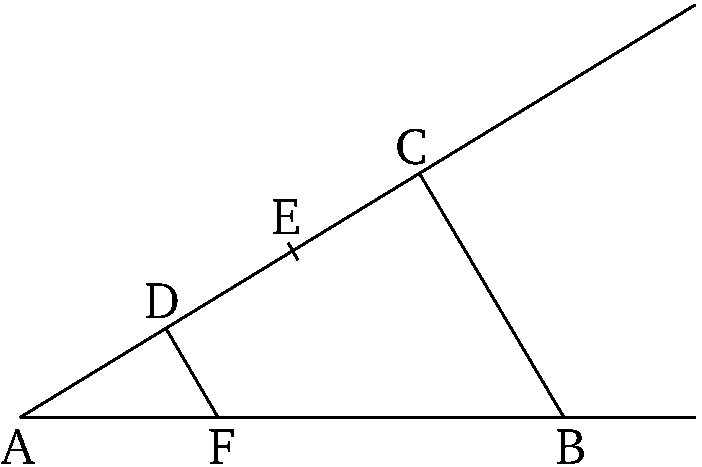
\includegraphics{Book06/fig09e.pdf}}

So let a third (part) be prescribed. [And] let some straight-line $AC$
be drawn from (point) $A$, encompassing a random angle with
$AB$.  And let a random point $D$ be taken on $AC$. And let
$DE$ and $EC$ be made equal to $AD$ [Prop.~1.3]. And let $BC$ be
joined. And let $DF$ be drawn through $D$ parallel to it [Prop.~1.31].

Therefore, since $FD$ has been drawn parallel to one of the sides, $BC$,
of triangle $ABC$, then, proportionally, as $CD$ is to $DA$, so $BF$ (is) to
$FA$ [Prop.~6.2].
And $CD$ (is) double $DA$.  Thus, $BF$ (is) also double $FA$. Thus, $BA$ (is)
triple $AF$.

Thus, the prescribed third part, $AF$, has been cut off from the given
straight-line, $AB$. (Which is) the very thing it was required to do.}
\end{Parallel}

%%%%%%
% Prop 6.10
%%%%%%
\pdfbookmark[1]{Proposition 6.10}{pdf6.10}
\begin{Parallel}{}{} 
\ParallelLText{
\begin{center}
{\large \ggn{10}.}
\end{center}\vspace*{-7pt}

\gr{Τὴν δοθεῖσαν εὐθεῖαν >άτμ\kern -.7pt  ητον τῆ| δοθείσῃ τετμ\kern -.7pt  ημένῃ ὁμοίωξ
τεμεῖν.}

\gr{>'Εστω ἡ μὲν δοθεῖσα εὐθεῖα <άτμ\kern -.7pt  ητοξ ἡ ΑΒ,
ἡ δὲ τετμ\kern -.7pt  ημένη ἡ ΑΓ κατὰ τὰ Δ, Ε σημεῖα, καὶ κείσθωσαν
<ώστε γωνίαν τυθοῦσαν περιέθειν, καὶ ἐπεζεύθθω ἡ ΓΒ, καὶ διὰ
τῶν Δ, Ε τῆ|  ΒΓ παράλληλοι >ήθθωσαν αἱ ΔΖ, ΕΗ, διὰ δὲ τοῦ Δ
τῆ| ΑΒ παράλληλοξ >ήθθω ἡ ΔΘΚ.}\\

% Removed epsf size command
\centerline{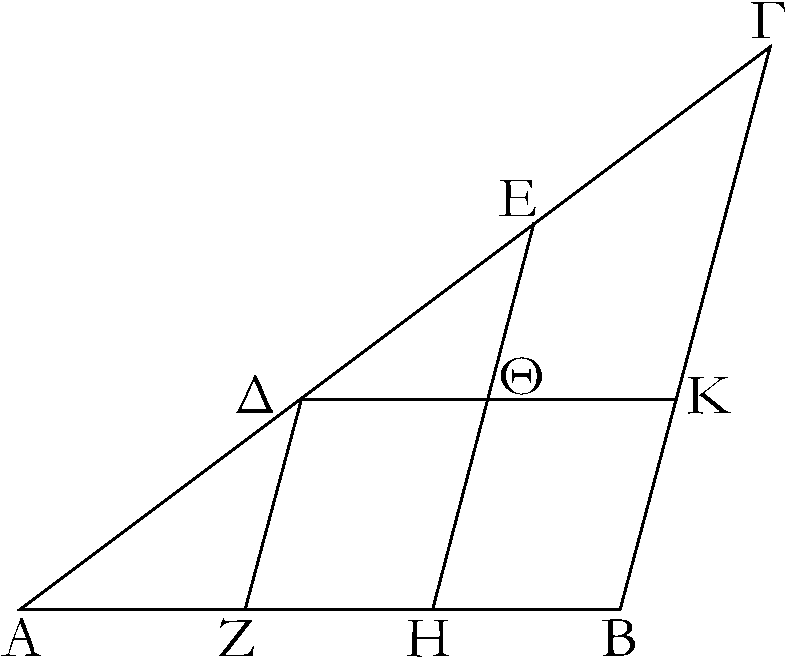
\includegraphics{Book06/fig10g.pdf}}

\gr{Παραλληλόγραμμον >άρα ἐστὶν ἑκάτερον τῶν ΖΘ, ΘΒ; >ίση
>άρα ἡ μὲν ΔΘ τῆ| ΖΗ, ἡ δὲ ΘΚ τῆ| ΗΒ. καὶ ἐπεὶ τριγώνου
τοῦ ΔΚΓ παρὰ μίαν τῶν πλευρῶν τὴν ΚΓ εὐθεῖα >ῆκται ἡ
ΘΕ, ἀνάλογον >άρα ἐστὶν ὡξ ἡ ΓΕ πρὸξ τὴν ΕΔ, ο<ύτωξ
ἡ ΚΘ πρὸξ τὴν ΘΔ. >ίση δὲ ἡ μὲν ΚΘ τῆ| ΒΗ, ἡ δὲ ΘΔ
τῆ| ΗΖ. >έστιν >άρα ὡξ ἡ ΓΕ πρὸξ τὴν ΕΔ, ο<ύτωξ
ἡ ΒΗ πρὸξ τὴν ΗΖ. πάλιν, ἐπεὶ τριγώνου τοῦ ΑΗΕ παρὰ μίαν
τῶν πλευρῶν τὴν ΗΕ >ῆκται ἡ ΖΔ, ἀνάλογον >άρα ἐστὶν ὡξ
ἡ ΕΔ πρὸξ τὴν ΔΑ, ο<ύτωξ ἡ ΗΖ πρὸξ τὴν ΖΑ. ἐδείθθη δὲ
καὶ ὡξ ἡ ΓΕ πρὸξ τὴν ΕΔ, ο<ύτωξ ἡ ΒΗ πρὸξ τὴν ΗΖ;
>έστιν >άρα ὡξ μὲν ἡ ΓΕ πρὸξ τὴν ΕΔ, ο<ύτωξ ἡ ΒΗ
πρὸξ τὴν ΗΖ, ὡξ δὲ ἡ ΕΔ πρὸξ τὴν ΔΑ, ο<ύτωξ ἡ ΗΖ
πρὸξ τὴν ΖΑ.}

\gr{Ἡ >άρα δοθεῖσα εὐθεῖα >άτμ\kern -.7pt  ητοξ ἡ ΑΒ τῆ| δοθείσῃ εὐθείᾳ
τετμ\kern -.7pt  ημένῃ τῆ| ΑΓ ὁμοίωξ τέτμ\kern -.5pt  ηται; <όπερ >έδει ποιῆσαι;}}

\ParallelRText{
\begin{center}
{\large Proposition 10}
\end{center}

To cut a given uncut  straight-line similarly
to a given cut (straight-line).

Let $AB$ be the given uncut straight-line, and $AC$ a  (straight-line) cut at
points $D$ and $E$, and let ($AC$) be laid down so as to encompass a random angle (with $AB$).  And let $CB$ be joined. And let $DF$ and $EG$ be
drawn through (points) $D$ and $E$ (respectively), parallel to $BC$, and let $DHK$
be drawn through (point) $D$, parallel to $AB$  [Prop.~1.31].

% Removed epsf size command
\centerline{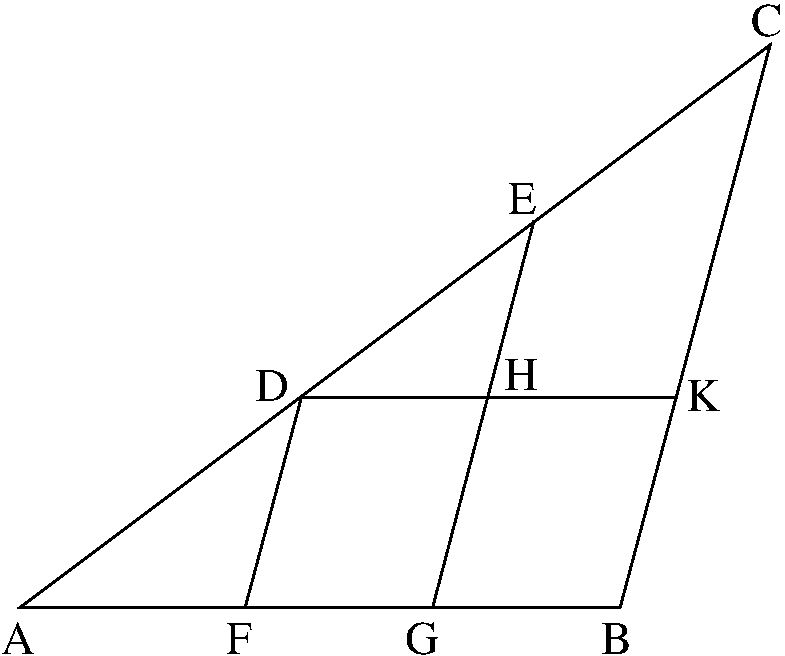
\includegraphics{Book06/fig10e.pdf}}

Thus, $FH$ and $HB$ are each parallelograms. Thus, $DH$ (is) equal to $FG$,
and $HK$ to $GB$ [Prop.~1.34]. 
And since the straight-line $HE$ has been drawn parallel to one of the
sides, $KC$, of triangle $DKC$, thus, proportionally, as $CE$ is to $ED$,  so $KH$
(is) to $HD$ [Prop.~6.2]. And $KH$ (is)
equal to $BG$, and $HD$ to $GF$. Thus, as $CE$ is to $ED$, so $BG$ (is) to $GF$. 
Again, since $FD$ has been drawn parallel to one of the sides, $GE$, of
triangle $AGE$, thus, proportionally, as $ED$ is to $DA$, so $GF$ (is) to $FA$
[Prop.~6.2]. And it was also shown
that as $CE$ (is) to $ED$, so $BG$ (is) to $GF$. Thus, as
$CE$ is to $ED$, so $BG$ (is) to $GF$, and as $ED$ (is) to $DA$, so $GF$ (is) to
$FA$.

Thus, the given uncut straight-line, $AB$, has been cut similarly
to the given cut straight-line, $AC$. (Which is) the very thing it was required to do.}
\end{Parallel}

%%%%%%
% Prop 6.11
%%%%%%
\pdfbookmark[1]{Proposition 6.11}{pdf6.11}
\begin{Parallel}{}{} 
\ParallelLText{
\begin{center}
{\large \ggn{11}.}
\end{center}\vspace*{-7pt}

\gr{Δύο δοθεισῶν εὐθειῶν τρίτην ἀνάλογον προσευρεῖν.}

\gr{>'Εστωσαν αἱ δοθεῖσαι [δύο εὐθεῖαι] αἱ ΒΑ, ΑΓ καὶ κείσθωσαν
γωνίαν περιέθουσαι τυθοῦσαν. δεῖ δὴ τῶν ΒΑ, ΑΓ τρίτην
ἀνάλογον προσευρεῖν. ἐκβεβλήσθωσαν γὰρ ἐπὶ τὰ Δ, Ε
σημεῖα, καὶ κείσθω τῆ| ΑΓ >ίση ἡ ΒΔ, καὶ
ἐπεζεύθθω ἡ ΒΓ, καὶ διὰ τοῦ Δ παράλληλοξ α\kern -.7pt  ὐτῆ|
>ήθθω ἡ ΔΕ.}\\~\\~\\

% Removed epsf size command
\centerline{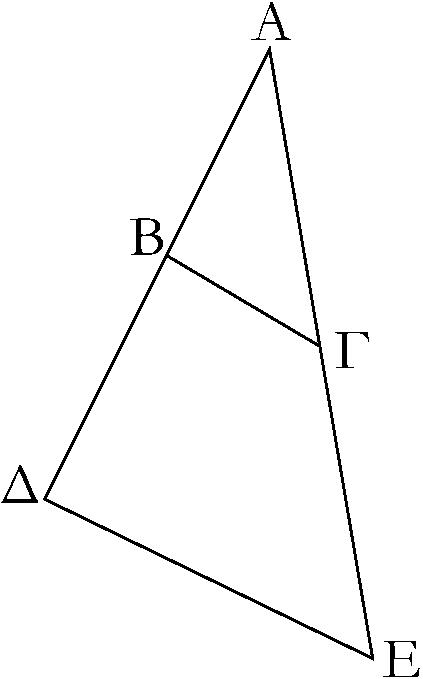
\includegraphics{Book06/fig11g.pdf}}

\gr{Ἐπεὶ ο>ῦν τριγώνου τοῦ ΑΔΕ παρὰ μίαν τῶν πλευρῶν τὴν
ΔΕ >ῆκται ἡ ΒΓ, ἀνάλογόν ἐστιν ὡξ ἡ ΑΒ πρὸξ τὴν ΒΔ,
ο<ύτωξ ἡ ΑΓ πρὸξ τὴν ΓΕ. >ίση δὲ ἡ ΒΔ τῆ| ΑΓ. >έστιν
>άρα ὡξ ἡ ΑΒ πρὸξ τὴν ΑΓ, ο<ύτωξ ἡ ΑΓ πρὸξ τὴν ΓΕ.}

\gr{Δύο >άρα δοθεισῶν εὐθειῶν τῶν ΑΒ, ΑΓ τρίτη ἀνάλογον
α\kern -.7pt  ὐταῖξ προσεύρηται ἡ ΓΕ; <όπερ >έδει ποιῆσαι.}}

\ParallelRText{
\begin{center}
{\large Proposition 11}
\end{center}

To find a third (straight-line) proportional to two
given straight-lines.

Let $BA$ and $AC$ be the [two] given [straight-lines], and let them be laid
down encompassing a random angle. So it is required to find
a third (straight-line) proportional to $BA$ and $AC$. For let ($BA$ and $AC$) 
be produced to points $D$ and $E$ (respectively), and let $BD$ be made equal
to $AC$  [Prop.~1.3]. And let $BC$ be joined. And let $DE$ be drawn
through (point) $D$ parallel to it [Prop.~1.31].

% Removed epsf size command
\centerline{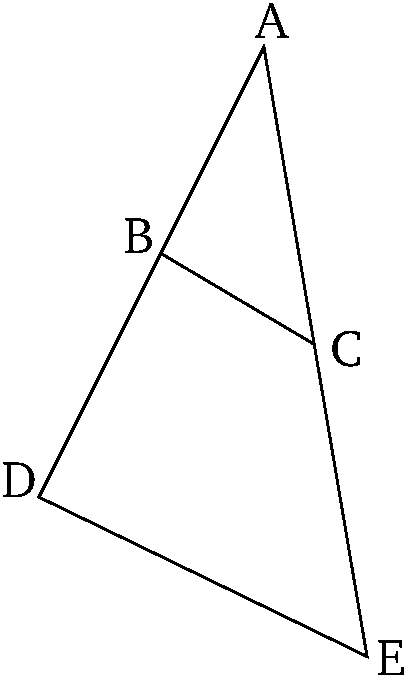
\includegraphics{Book06/fig11e.pdf}}

Therefore, since $BC$
has been drawn parallel to one of the sides $DE$ of triangle $ADE$, proportionally, as $AB$ is to $BD$, so $AC$ (is) to $CE$ [Prop.~6.2]. And $BD$ (is) equal to $AC$.
Thus, as $AB$ is to $AC$, so $AC$ (is) to $CE$.

Thus, a third (straight-line), $CE$, has been found (which is) proportional to the two
given straight-lines, $AB$ and $AC$. (Which is) the very thing it was required to
do.}
\end{Parallel}

%%%%%%
% Prop 6.12
%%%%%%
\pdfbookmark[1]{Proposition 6.12}{pdf6.12}
\begin{Parallel}{}{} 
\ParallelLText{
\begin{center}
{\large \ggn{12}.}
\end{center}\vspace*{-7pt}

\gr{Τριῶν δοθεισῶν εὐθειῶν τετάρτην ἀνάλογον προσευρεῖν.}\\

% Removed epsf size command
\centerline{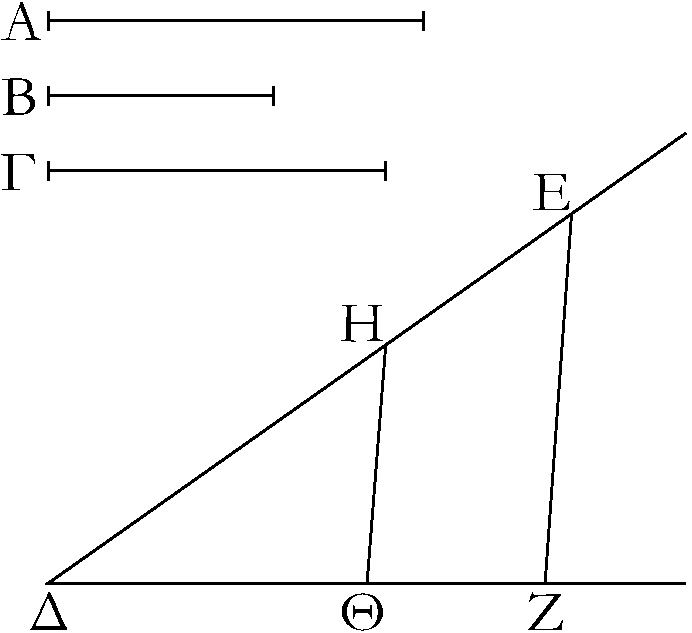
\includegraphics{Book06/fig12g.pdf}}

\gr{>'Εστωσαν αἱ δοθεῖσαι τρεῖξ εὐθεῖαι αἱ Α, Β, Γ; δεῖ δὴ τῶν
Α, Β, Γ τετράτην ἀνάλογον προσευρεῖν.}

\gr{Ἐκκείσθωσαν δύο εὐθεῖαι αἱ ΔΕ, ΔΖ γωνίαν περιέθουσαι [τυθοῦσαν]
τὴν ὑπὸ ΕΔΖ; καὶ κείσθω τῆ| μὲν Α >ίση ἡ ΔΗ, τῆ| δὲ Β >ίση
ἡ ΗΕ, καὶ >έτι τῆ| Γ >ίση ἡ ΔΘ; καὶ ἐπιζευθθείσηξ τῆξ ΗΘ παράλληλοξ
α\kern -.7pt  ὐτῆ| >ήθθω διὰ τοῦ Ε ἡ ΕΖ.}

\gr{Ἐπεὶ ο>ῦν τριγώνου τοῦ ΔΕΖ παρὰ μίαν τὴν ΕΖ >ῆκται ἡ ΗΘ,
>έστιν >άρα ὡξ ἡ ΔΗ πρὸξ τὴν ΗΕ, ο<ύτωξ ἡ ΔΘ πρὸξ τὴν
ΘΖ. >ίση δὲ ἡ μὲν ΔΗ τῆ| Α, ἡ δὲ ΗΕ τῆ| Β, ἡ δὲ ΔΘ τῆ|
Γ; >έστιν >άρα ὡξ ἡ Α πρὸξ τὴν Β, ο<ύτωξ ἡ Γ πρὸξ τὴν ΘΖ.}

\gr{Τριῶν >άρα δοθεισῶν εὐθειῶν τῶν Α, Β, Γ τετάρτη ἀνάλογον
προσεύρηται ἡ ΘΖ; <όπερ >έδει ποιῆσαι.}}

\ParallelRText{
\begin{center}
{\large Proposition 12}
\end{center}

To find a fourth (straight-line) proportional
to three given straight-lines.

% Removed epsf size command
\centerline{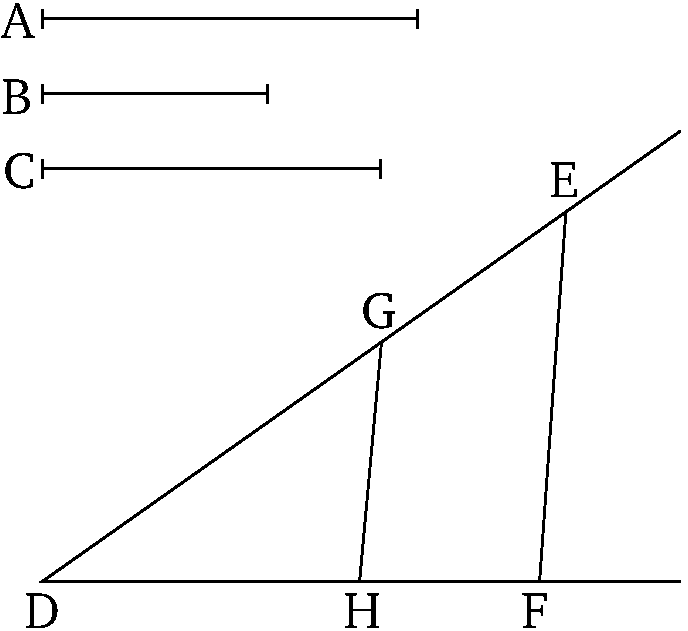
\includegraphics{Book06/fig12e.pdf}}

Let $A$, $B$, and $C$ be the three given straight-lines. So it is required
to find a fourth (straight-line) proportional to $A$, $B$, and $C$.

Let the two straight-lines $DE$ and $DF$ be set out encompassing the
[random] angle $EDF$. And let $DG$ be made equal to $A$, and $GE$ to $B$,
and, further, $DH$ to $C$  [Prop.~1.3]. And $GH$ being joined, 
let $EF$ be drawn through (point) $E$ parallel to it  [Prop.~1.31].

Therefore, since $GH$ has been drawn parallel to one of the sides $EF$ of 
triangle $DEF$, thus as $DG$ is to $GE$, so $DH$ (is) to $HF$ [Prop.~6.2]. And $DG$ (is) equal to $A$, and
$GE$ to $B$, and $DH$ to $C$. Thus, as $A$ is to $B$, so $C$ (is) to $HF$.

Thus, a fourth (straight-line), $HF$, has been found (which is) proportional to the three given
straight-lines, $A$, $B$, and $C$. (Which is) the very thing it was required to
do.}
\end{Parallel}

%%%%%%
% Prop 6.13
%%%%%%
\pdfbookmark[1]{Proposition 6.13}{pdf6.13}
\begin{Parallel}{}{} 
\ParallelLText{
\begin{center}
{\large \ggn{13}.}
\end{center}\vspace*{-7pt}

\gr{Δύο δοθεισῶν εὐθειῶν μέσην ἀνάλογον προσευρεῖν.}\\

% Removed epsf size command
\centerline{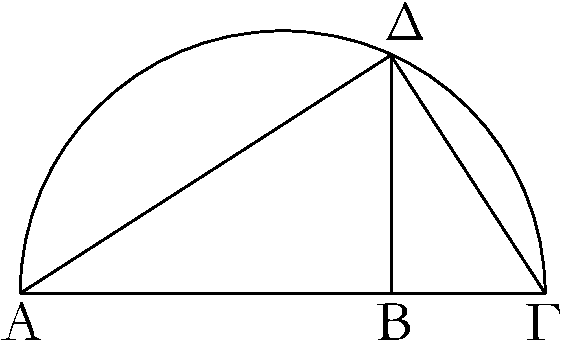
\includegraphics{Book06/fig13g.pdf}}

\gr{>'Εστωσαν αἱ δοθεῖσαι δύο εὐθεῖαι αἱ ΑΒ, ΒΓ; δεῖ δὴ τῶν
ΑΒ, ΒΓ μέσην ἀνάλογον προσευρεῖν.}

\gr{Κείσθωσαν ἐπ> εὐθείαξ, καὶ γεγράφθω ἐπὶ τῆξ ΑΓ ἡμικύκλιον
τὸ ΑΔΓ, καὶ >ήθθω ἀπὸ τοῦ Β σημείου τῆ| ΑΓ εὐθείᾳ πρὸξ
ὀρθὰξ ἡ ΒΔ, καὶ ἐπεζεύθθωσαν αἱ ΑΔ, ΔΓ.}

\gr{Ἐπεὶ ἐν ἡμικυκλίῳ γωνία ἐστὶν ἡ ὑπὸ ΑΔΓ,
ὀρθή ἐστιν. καὶ ἐπεὶ ἐν ὀρθογωνίῳ τριγώνῳ τῶ|
ΑΔΓ ἀπὸ τῆξ ὀρθῆξ γωνίαξ ἐπὶ τὴν βάσιν κάθετοξ
>ῆκται ἡ ΔΒ, ἡ ΔΒ >άρα τῶν τῆξ βάσεωξ τμ\kern -.7pt  ημάτων
τῶν ΑΒ, ΒΓ μέση ἀνάλογόν ἐστιν.}

\gr{Δύο >άρα δοθεισῶν εὐθειῶν τῶν ΑΒ, ΒΓ μέση ἀνάλογον
προσεύρηται ἡ ΔΒ; <όπερ >έδει ποιῆσαι.}}

\ParallelRText{
\begin{center}
{\large Proposition 13}
\end{center}

To find the (straight-line) in mean proportion to two
given straight-lines.$^\dag$

% Removed epsf size command
\centerline{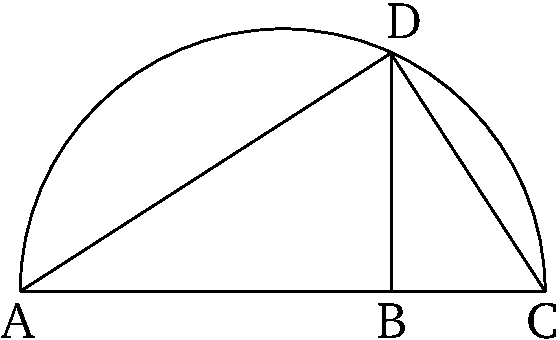
\includegraphics{Book06/fig13e.pdf}}

Let $AB$ and $BC$ be the two given straight-lines. So it is required to
find the (straight-line) in mean proportion to $AB$ and $BC$.

Let  ($AB$ and $BC$) be laid down straight-on (with respect to one another), and
let the semi-circle $ADC$ be drawn on $AC$  [Prop.~1.10]. And let $BD$ be drawn
from (point) $B$, at right-angles to $AC$  [Prop.~1.11]. And let $AD$ and $DC$ be joined.

And since $ADC$ is an angle in a semi-circle, it is a right-angle  [Prop.~3.31].
 And since, in the right-angled triangle $ADC$,  the (straight-line) $DB$ has been drawn from the right-angle perpendicular
  to the base, $DB$ is thus the mean proportional to the pieces of the base,  $AB$ and $BC$ 
[Prop.~6.8~corr.].

Thus, $DB$ has been found (which is) in mean proportion to the two given
straight-lines, $AB$ and $BC$. (Which is) the very thing it was required to
do.}
\end{Parallel}
{\footnotesize\noindent $^\dag$ In other words, to find the geometric mean of
two given straight-lines.}

%%%%%%
% Prop 6.14
%%%%%%
\pdfbookmark[1]{Proposition 6.14}{pdf6.14}
\begin{Parallel}{}{} 
\ParallelLText{
\begin{center}
{\large \ggn{14}.}
\end{center}\vspace*{-7pt}

\gr{Τῶν >ίσων τε καὶ >ίσογωνίων παραλληλογράμμων ἀντιπεπόνθασιν
αἱ πλευραὶ αἱ περὶ τὰξ >ίσαξ γωνίαξ; καὶ <ῶν ἰσογωνίων
παραλληλογράμμων ἀντιπεπόνθασιν αἱ πλευραὶ αἱ περὶ τὰξ
>ίσαξ γωνίαξ, >ίσα ἐστὶν ἐκεῖνα.}

\gr{>'Εστω >ίσα τε καὶ ἰσογώνια παραλληλόγραμμα τὰ ΑΒ, ΒΓ >ίσαξ >έθοντα
τὰξ πρὸξ τῶ| Β γωνίαξ, καὶ κείσθωσαν ἐπ> εὐθείαξ αἱ ΔΒ, ΒΕ;
ἐπ> εὐθείαξ >άρα εἰσὶ καὶ αἱ ΖΒ, ΒΗ. λέγω, <ότι τῶν ΑΒ, ΒΓ
ἀντιπεπόνθασιν αἱ πλευραὶ αἱ περὶ τὰξ >ίσαξ γωνίαξ,
τουτέστιν, <ότι ἐστὶν ὡξ ἡ ΔΒ πρὸξ τὴν ΒΕ, ο<ύτωξ
ἡ ΗΒ πρὸξ τὴν ΒΖ.}\\

% Removed epsf size command
\centerline{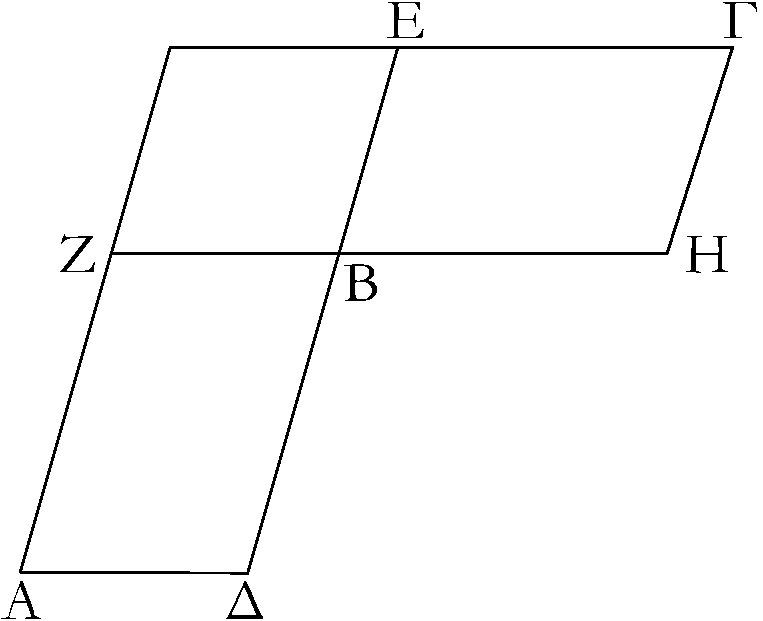
\includegraphics{Book06/fig14g.pdf}}

\gr{Συμπεπληρώσθω γὰρ τὸ ΖΕ παραλληλόγραμμον. ἐπεὶ ο>ῦν >ίσον
ἐστὶ τὸ ΑΒ παραλληλόγραμμον τῶ| ΒΓ παραλληλογράμμῳ,
>άλλο δέ τι τὸ ΖΕ, >έστιν >άρα ὡξ τὸ ΑΒ πρὸξ τὸ ΖΕ, ο<ύτωξ
τὸ ΒΓ πρὸξ τὸ ΖΕ. ἀλλ> ὡξ μὲν τὸ ΑΒ πρὸξ τὸ ΖΕ, ο<ύτωξ
ἡ ΔΒ πρὸξ τὴν ΒΕ, ὡξ δὲ τὸ ΒΓ πρὸξ τὸ ΖΕ, ο<ύτωξ ἡ
ΗΒ πρὸξ τὴν ΒΖ; καὶ ὡξ >άρα ἡ ΔΒ πρὸξ τὴν ΒΕ,
ο<ύτωξ ἡ ΗΒ πρὸξ τὴν ΒΖ. τῶν >άρα ΑΒ, ΒΓ παραλληλογράμμων
ἀντιπεπόνθασιν αἱ πλευραὶ αἱ περὶ τὰξ >ίσαξ γωνίαξ.}

\gr{Ἀλλὰ δὴ >έστω ὡξ ἡ ΔΒ πρὸξ τὴν ΒΕ, ο<ύτωξ ἡ ΗΒ
πρὸξ τὴν ΒΖ; λέγω, <ότι >ίσον ἐστὶ τὸ ΑΒ παραλληλόγραμμον τῶ|
ΒΓ παραλληλογράμμῳ.}

\gr{Ἐπεὶ γάρ ἐστιν ὡξ ἡ ΔΒ πρὸξ τὴν ΒΕ, ο<ύτωξ ἡ ΗΒ πρὸξ
τὴν ΒΖ, ἀλλ> ὡξ μὲν ἡ ΔΒ πρὸξ τὴν  ΒΕ, ο<ύτωξ τὸ ΑΒ
παραλληλόγραμμον πρὸξ τὸ ΖΕ παραλληλόγραμμον, ὡξ δὲ ἡ ΗΒ πρὸξ
τὴν ΒΖ, ο<ύτωξ τὸ ΒΓ παραλληλόγραμμον πρὸξ τὸ ΖΕ παραλληλόγραμμον,
καὶ ὡξ >άρα τὸ ΑΒ πρὸξ τὸ ΖΕ, ο<ύτωξ τὸ ΒΓ πρὸξ τὸ ΖΕ;
>ίσον >άρα ἐστὶ τὸ ΑΒ παραλληλόγραμμον τῶ| ΒΓ παραλληλογράμμῳ.}

\gr{Τῶν >άρα >ίσων τε καὶ ἰσογωνίων παραλληλογράμμων ἀντιπεπόνθασιν
αἱ πλευραὶ αἱ περὶ τὰξ >ίσαξ γωνίαξ; καὶ <ῶν ἰσογωνίων
παραλληλογράμμων ἀντιπεπόνθασιν αἱ πλευραὶ αἱ περὶ τὰξ
>ίσαξ γωνίαξ, >ίσα ἐστὶν ἐκεῖνα; <όπερ >έδει δεῖχαι.}}

\ParallelRText{
\begin{center}
{\large Proposition 14}
\end{center}

In equal and equiangular parallelograms, the
sides about the equal angles are reciprocally proportional. And those
equiangular parallelograms in which  the sides about the equal
angles are reciprocally proportional are equal.

Let $AB$ and $BC$ be equal and equiangular parallelograms having the angles
at $B$ equal. And let $DB$ and $BE$ be laid down straight-on (with respect to one
another). Thus, $FB$ and $BG$ are also straight-on (with respect to one another)  [Prop.~1.14].
I say that the sides of $AB$ and $BC$ about the equal angles
are reciprocally proportional, that is to say, that as $DB$ is to $BE$,
so $GB$ (is) to $BF$.

% Removed epsf size command
\centerline{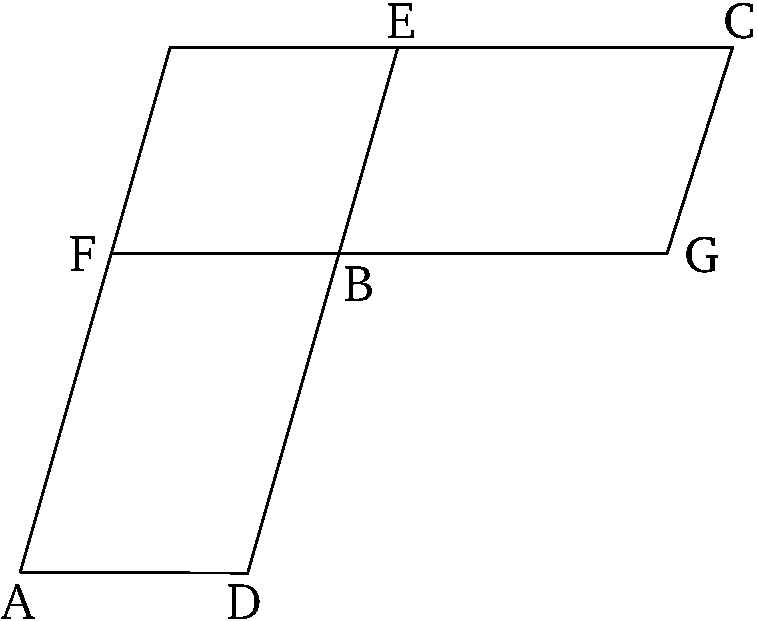
\includegraphics{Book06/fig14e.pdf}}

For let the parallelogram $FE$ be completed. Therefore, since parallelogram $AB$ is equal to parallelogram $BC$, and $FE$ (is) some
other (parallelogram), thus as (parallelogram) $AB$ is to $FE$, so (parallelogram) $BC$ (is) to $FE$ [Prop.~5.7]. But, as (parallelogram) $AB$ (is) to $FE$, so $DB$
(is) to $BE$, and as (parallelogram) $BC$ (is) to $FE$, so $GB$ (is) to $BF$ [Prop.~6.1]. Thus, also, as $DB$ (is) to
$BE$, so $GB$ (is) to $BF$. Thus, in parallelograms $AB$ and $BC$
the sides about the equal angles are reciprocally proportional.

And so, let $DB$ be to $BE$, as $GB$ (is) to $BF$. I say that parallelogram
$AB$ is equal to parallelogram $BC$.

For since as $DB$ is to $BE$, so $GB$ (is) to $BF$, but as $DB$ (is) to $BE$, so
parallelogram $AB$ (is) to parallelogram $FE$, and as $GB$ (is) to $BF$,
so parallelogram $BC$ (is) to parallelogram $FE$  [Prop.~6.1], thus, also, as (parallelogram) $AB$ (is)
to $FE$, so (parallelogram) $BC$ (is) to $FE$ [Prop.~5.11].
Thus,  parallelogram $AB$ is equal to parallelogram $BC$ [Prop.~5.9].

Thus, in equal and equiangular parallelograms, the
sides about the equal angles are reciprocally proportional. And those
equiangular parallelograms in which the sides about the equal
angles are reciprocally proportional are equal. (Which is) the very thing
it was required to show.}
\end{Parallel}

%%%%%%
% Prop 6.15
%%%%%%
\pdfbookmark[1]{Proposition 6.15}{pdf6.15}
\begin{Parallel}{}{} 
\ParallelLText{
\begin{center}
{\large \ggn{15}.}
\end{center}\vspace*{-7pt}

\gr{Τῶν >ίσων καὶ μίαν μιᾶ| >ίσην ἐθόντων γωνίαν τριγώνων
ἀντιπεπόνθασιν αἱ πλευραὶ αἱ περὶ τὰξ >ίσαξ γωνίαξ; καὶ <ῶν
μίαν μιᾶ| >ίσην ἐθόντων γωνίαν τριγώνων ἀντιπεπόνθασιν
αἱ πλευραὶ αἱ περὶ τὰξ >ίσαξ γωνίαξ, >ίσα ἐστὶν ἐκεῖνα.}

\gr{>'Εστω >ίσα τρίγωνα τὰ ΑΒΓ, ΑΔΕ μίαν μιᾶ| >ίσην
>έθοντα γωνίαν τὴν ὑπὸ ΒΑΓ τῆ| ὑπὸ ΔΑΕ; λέγω,
<ότι τῶν ΑΒΓ, ΑΔΕ τριγώνων ἀντιπεπόνθασιν αἱ πλευραὶ
αἱ περὶ τὰξ >ίσαξ γωνίαξ, τουτέστιν, <ότι ἐστὶν ὡξ ἡ ΓΑ
πρὸξ τὴν ΑΔ, ο<ύτωξ ἡ ΕΑ πρὸξ τὴν ΑΒ.}\\

% Removed epsf size command
\centerline{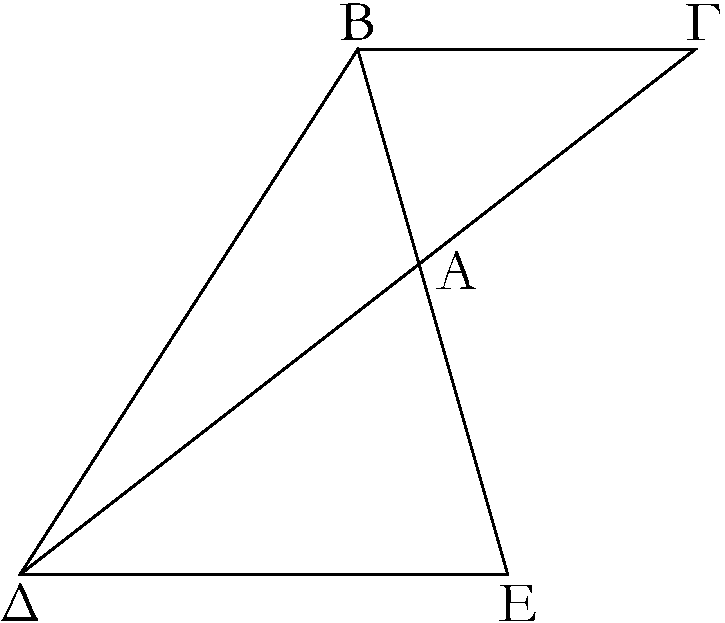
\includegraphics{Book06/fig15g.pdf}}

\gr{Κείσθω γὰρ <ώστε ἐπ> εὐθείαξ ε>ῖναι τὴν ΓΑ τῆ| ΑΔ;
ἐπ> εὐθείαξ >άρα ἐστὶ καὶ ἡ ΕΑ τῆ| ΑΒ. καὶ ἐπεζεύθθω
ἡ ΒΔ.}

\gr{Ἐπεὶ ο>ῦν >ίσον ἐστὶ τὸ ΑΒΓ τρίγωνον τῶ| ΑΔΕ τριγώνῳ,
>άλλο δέ τι τὸ ΒΑΔ, >έστιν >άρα ὡξ τὸ ΓΑΒ τρίγωνον
πρὸξ τὸ ΒΑΔ τρίγωνον, ο<ύτωξ τὸ ΕΑΔ τρίγωνον πρὸξ τὸ
ΒΑΔ τρίγωνον. ἀλλ> ὡξ μὲν τὸ ΓΑΒ πρὸξ τὸ ΒΑΔ, 
ο<ύτωξ ἡ ΓΑ πρὸξ τὴν ΑΔ, ὡξ δὲ τὸ ΕΑΔ πρὸξ τὸ
ΒΑΔ, ο<ύτωξ ἡ ΕΑ πρὸξ τὴν ΑΒ. καὶ ὡξ >άρα ἡ ΓΑ πρὸξ
τὴν ΑΔ, ο<ύτωξ ἡ ΕΑ πρὸξ τὴν ΑΒ. τῶν ΑΒΓ, ΑΔΕ
>άρα τριγώνων ἀντιπεπόνθασιν αἱ πλευραὶ αἱ περὶ τὰξ >ίσαξ
γωνίαξ.}

\gr{Ἀλλὰ δὴ ἀντιπεπονθέτωσαν αἱ πλευραὶ τῶν ΑΒΓ, ΑΔΕ τριγώνων, καὶ
>έστω ὡξ ἡ ΓΑ πρὸξ τὴν ΑΔ, ο<ύτωξ ἡ ΕΑ πρὸξ τὴν ΑΒ;
λέγω, <ότι >ίσον ἐστὶ τὸ ΑΒΓ τρίγωνον τῶ| ΑΔΕ τριγώνῳ.}

\gr{Ἐπιζευθθείσηξ γὰρ πάλιν τῆξ ΒΔ, ἐπεί ἐστιν ὡξ
ἡ ΓΑ πρὸξ τὴν ΑΔ, ο<ύτωξ ἡ ΕΑ πρὸξ τὴν ΑΒ, ἀλλ> ὡξ μὲν
ἡ ΓΑ πρὸξ τὴν ΑΔ, ο<ύτωξ τὸ ΑΒΓ
τρίγωνον πρὸξ τὸ ΒΑΔ τρίγωνον, ὡξ δὲ ἡ ΕΑ πρὸξ
τὴν ΑΒ, ο<ύτωξ τὸ ΕΑΔ τρίγωνον πρὸξ τὸ ΒΑΔ τρίγωνον, 
ὡξ >άρα τὸ ΑΒΓ τρίγωνον πρὸξ τὸ ΒΑΔ τρίγωνον,
ο<ύτωξ
τὸ ΕΑΔ τρίγωνον πρὸξ τὸ ΒΑΔ τρίγωνον. ἑκάτερον >άρα
τῶν ΑΒΓ, ΕΑΔ πρὸξ τὸ ΒΑΔ τὸν α\kern -.7pt  ὐτὸν >έθει λόγον. >ίσων
>άρα ἐστὶ τὸ ΑΒΓ [τρίγωνον] τῶ| ΕΑΔ τριγώνῳ.}

\gr{Τῶν >άρα >ίσων καὶ μίαν μιᾶ| >ίσην ἐθόντων γωνίαν τριγώνων
ἀντιπεπόνθασιν αἱ πλευραὶ αἱ περὶ τὰξ >ίσαξ γωνίαξ; καὶ <ῶξ
μίαν μιᾶ| >ίσην ἐθόντων γωνίαν τριγώνων ἀντιπεπόνθασιν
αἱ πλευραὶ αἱ περὶ τὰξ >ίσαξ γωνίαξ,  ἐκεῖνα  >ίσα ἐστὶν;
<όπερ >έδει δεῖχαι.}}

\ParallelRText{
\begin{center}
{\large Proposition 15}
\end{center}

In equal triangles also having one angle equal to
one (angle), the sides about the equal angles are reciprocally proportional.
And those triangles having one angle equal to one angle for which 
the sides about the equal angles (are) reciprocally proportional are equal.

Let $ABC$ and $ADE$ be equal triangles having one angle equal to
one (angle), (namely) $BAC$ (equal) to $DAE$. I say that, in triangles
$ABC$ and $ADE$, the sides about the equal angles are reciprocally
proportional, that is to say, that as $CA$ is to $AD$, so $EA$ (is) to $AB$.

% Removed epsf size command
\centerline{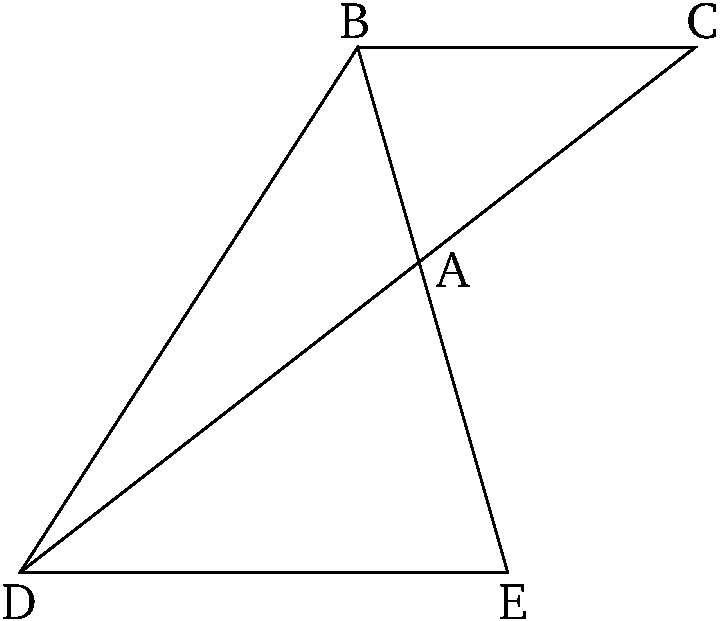
\includegraphics{Book06/fig15e.pdf}}

For let  $CA$ be laid down so as to be  straight-on (with respect) to $AD$. Thus,
$EA$ is also straight-on (with respect) to $AB$ 
[Prop.~1.14]. And let $BD$ be joined.

Therefore, since triangle $ABC$ is equal to triangle $ADE$, and
$BAD$ (is) some other (triangle), thus as triangle $CAB$ is
to triangle $BAD$, so triangle $EAD$ (is) to triangle $BAD$  [Prop.~5.7]. But, as (triangle)
$CAB$ (is) to $BAD$, so $CA$ (is) to $AD$, and as (triangle) $EAD$ (is) to $BAD$, so
$EA$ (is) to $AB$
[Prop.~6.1]. And thus, as $CA$ (is) to $AD$,
so $EA$ (is) to $AB$.  
Thus,  in triangles $ABC$ and
$ADE$ the sides about the equal angles (are) reciprocally proportional.

And so, let the sides of triangles $ABC$ and $ADE$ be reciprocally
proportional, and (thus) let $CA$ be to $AD$, as $EA$ (is) to $AB$. I say
that triangle $ABC$ is equal to triangle $ADE$.

For, $BD$ again being  joined, since as $CA$ is to $AD$, so $EA$ (is) to $AB$,
but as $CA$ (is) to $AD$, so triangle $ABC$ (is) to triangle
$BAD$, and as $EA$ (is) to $AB$, so triangle $EAD$ (is) to triangle $BAD$ 
[Prop.~6.1], thus as triangle
$ABC$ (is) to triangle $BAD$, so triangle $EAD$ (is) to triangle $BAD$. 
Thus, (triangles) $ABC$ and $EAD$ each have the same ratio to $BAD$. 
Thus, [triangle] $ABC$ is equal to triangle $EAD$ [Prop.~5.9].

Thus, in equal triangles also having one angle equal to
one (angle), the sides about the equal angles (are) reciprocally proportional.
And those triangles having one angle equal to one angle for which 
the sides about the equal angles (are) reciprocally proportional are equal.
(Which is) the very thing it was required to show.}
\end{Parallel}

%%%%%%
% Prop 6.16
%%%%%%
\pdfbookmark[1]{Proposition 6.16}{pdf6.16}
\begin{Parallel}{}{} 
\ParallelLText{
\begin{center}
{\large \ggn{16}.}
\end{center}\vspace*{-7pt}

\gr{Ἐὰν τέσσαρεξ εὐθεῖαι ἀνάλογον >ῶσιν, τὸ ὑπὸ τῶν >άκρων
περιεχόμενον ὀρθογώνιον >ίσον ἐστὶ τῶ| ὑπὸ τῶν μέσων
περιεθομένῳ ὀρθογωνίῳ; κ>ὰν τὸ ὑπὸ τῶν >άκρων περιεχόμενον
ὀρθογώνιον >ίσον >ῆ| τῶ| ὑπὸ τῶν μέσων περιεθομένῳ
ὀρθογωνίῳ, αἱ τέσσαρεξ εὐθεῖαι ἀνάλογον >έσονται.}\\

% Removed epsf size command
\centerline{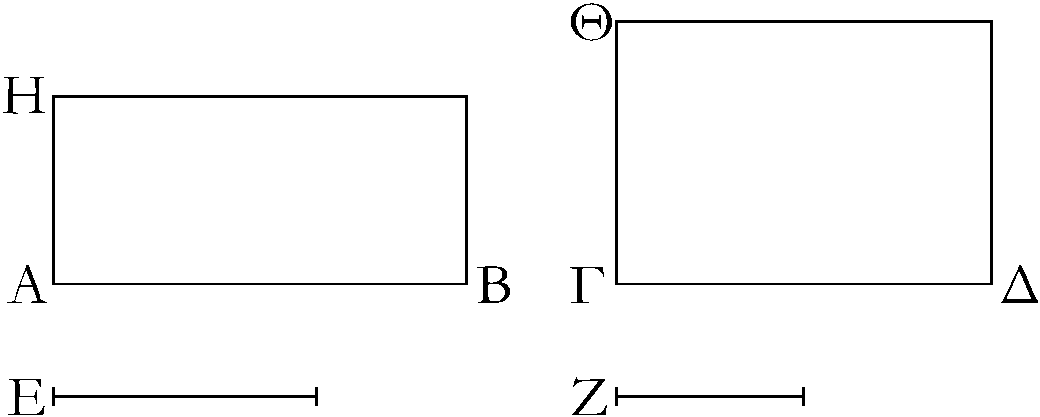
\includegraphics{Book06/fig16g.pdf}}

\gr{>'Εστωσαν τέσσαρεξ εὐθεῖαι ἀνάλογον αἱ ΑΒ, ΓΔ,
Ε, Ζ, ὡξ ἡ ΑΒ πρὸξ τὴν ΓΔ, ο<ύτωξ ἡ Ε
πρὸξ τὴν Ζ; λέγω, <ότι τὸ ὑπὸ τῶν ΑΒ, Ζ περιεχόμενον ὀρθογώνιον
>ίσον ἐστὶ τῶ| ὑπὸ τῶν ΓΔ, Ε περιεθομένῳ ὀρθογωνίῳ.}

\gr{>'Ηθθωσαν [γὰρ] ἀπὸ τῶν Α, Γ σημείων ταῖξ ΑΒ, ΓΔ εὐθείαιξ
πρὸξ ὀρθὰξ αἱ ΑΗ, ΓΘ, καὶ κείσθω τῆ| μὲν Ζ >ίση ἡ ΑΗ, τῆ| δὲ
Ε >ίση ἡ ΓΘ. καὶ συμπεπληρώσθω τὰ ΒΗ, ΔΘ παραλληλόγραμμα.}

\gr{Καὶ ἐπεί ἐστιν ὡξ ἡ ΑΒ πρὸξ τὴν ΓΔ, ο<ύτωξ ἡ Ε πρὸξ τὴν
Ζ, >ίση δὲ ἡ μὲν Ε τῆ| ΓΘ, ἡ δὲ Ζ τῆ| ΑΗ, >έστιν >άρα ὡξ ἡ ΑΒ
πρὸξ τὴν ΓΔ, ο<ύτωξ ἡ ΓΘ πρὸξ τὴν ΑΗ. τῶν ΒΗ, ΔΘ >άρα
παραλληλογράμμων ἀντιπεπόνθασιν αἱ πλευραὶ αἱ περὶ τὰξ >ίσαξ
γωνίαξ. <ῶν δὲ ἰσογωνίων παραλληλογράμμων ἀντιπεπόνθασιν
αἱ πλευραί αἱ περὶ τὰξ >ίσαξ γωνάιξ, >ίσα ἐστὶν ἐκεῖνα;
>ίσον >άρα ἐστὶ τὸ ΒΗ παραλληλόγραμμον τῶ| ΔΘ παραλληλογράμμῳ.
καί ἐστι τὸ μὲν ΒΗ τὸ ὑπὸ τῶν ΑΒ, Ζ; >ίση γὰρ ἡ ΑΗ τῆ| Ζ;
τὸ δὲ ΔΘ τὸ ὑπὸ τῶν ΓΔ, Ε; >ίση γὰρ ἡ Ε τῆ| ΓΘ; τὸ >άρα ὑπὸ
τῶν ΑΒ, Ζ περιεχόμενον ὀρθογώνιον >ίσον ἐστὶ τῶ| ὑπὸ τῶν
ΓΔ, Ε περιεθομένῳ ὀρθογώνιῳ.}

\gr{Ἀλλὰ δὴ τὸ ὑπὸ τῶν ΑΒ, Ζ περιεχόμενον ὀρθογώνιον >ίσον
>έστω τῶ| ὑπὸ τῶν ΓΔ, Ε περιεθομένῳ ὀρθογωνίῳ. λέγω,
<ότι αἱ τέσσαρεξ εὐθεῖαι ἀνάλογον >έσονται, ὡξ ἡ ΑΒ πρὸξ τὴν
ΓΔ, ο<ύτωξ ἡ Ε πρὸξ τὴν Ζ.}

\gr{Τῶν γὰρ α\kern -.7pt  ὐτῶν κατασκευασθέντων, ἐπεὶ τὸ ὑπὸ τῶν ΑΒ, Ζ
>ίσον ἐστὶ τῶ| ὑπὸ τῶν ΓΔ, Ε, καί ἐστι τὸ μὲν ὑπὸ τῶν
ΑΒ, Ζ τὸ ΒΗ; >ίση γάρ ἐστιν ἡ ΑΗ τῆ| Ζ; τὸ δὲ ὑπὸ τῶν ΓΔ, Ε
τὸ ΔΘ; >ίση γὰρ ἡ ΓΘ τῆ| Ε; τὸ >άρα ΒΗ >ίσον ἐστὶ τῶ| ΔΘ. καί
ἐστιν ἰσογώνια. τῶν δὲ >ίσων καὶ ἰσογωνίων παραλληλογράμμων
ἀντιπεπόνθασιν αἱ πλευραὶ αἱ περὶ τὰξ >ίσαξ
γωνίαξ. >έστιν >άρα ὡξ ἡ ΑΒ πρὸξ τὴν ΓΔ, ο<ύτωξ ἡ
ΓΘ πρὸξ τὴν ΑΗ. >ίση δὲ ἡ μὲν ΓΘ τῆ| Ε, ἡ δὲ ΑΗ τῆ| Ζ;
>έστιν >άρα ὡξ ἡ ΑΒ πρὸξ τὴν ΓΔ, ο<ύτωξ ἡ Ε
πρὸξ τὴν Ζ.}

\gr{Ἐὰν >άρα τέσσαρεξ εὐθεῖαι ἀνάλογον >ῶσιν, τὸ ὑπὸ τῶν >άκρων
περιεχόμενον ὀρθογώνιον >ίσον ἐστὶ τῶ| ὑπὸ τῶν μέσων
περιεθομένῳ ὀρθογωνίῳ; κ>ὰν τὸ ὑπὸ τῶν >άκρων περιεχόμενον
ὀρθογώνιον >ίσον >ῆ| τῶ| ὑπὸ τῶν μέσων περιεθομένῳ
ὀρθογωνίῳ, αἱ τέσσαρεξ εὐθεῖαι ἀνάλογον >έσονται; <όπερ >έδει
δεῖχαι.}}

\ParallelRText{
\begin{center}
{\large Proposition 16}
\end{center}

If four straight-lines are proportional, (then) the
rectangle contained by the (two) outermost is equal to the rectangle contained
by the middle (two). And if the rectangle contained by the (two) outermost
is
equal to the rectangle contained by the middle (two), (then) the four straight-lines
will be proportional.

% Removed epsf size command
\centerline{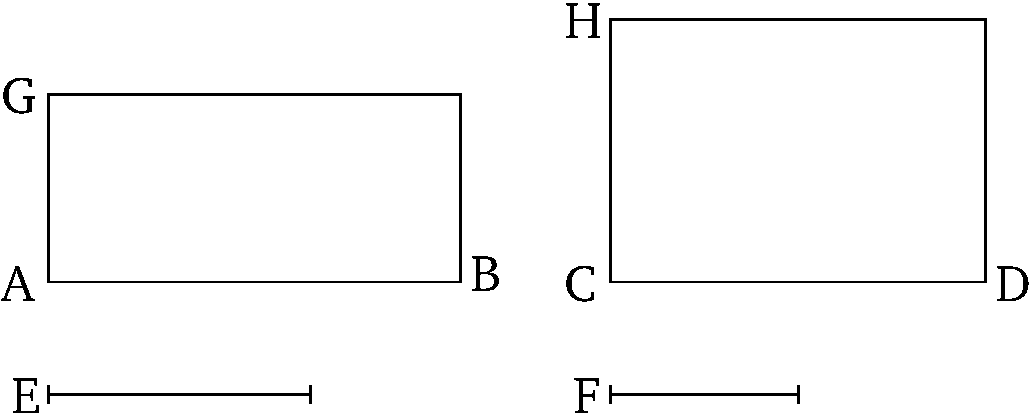
\includegraphics{Book06/fig16e.pdf}}

Let $AB$, $CD$, $E$, and $F$ be four proportional straight-lines, (such
that) as $AB$ (is) to $CD$, so $E$ (is) to $F$. I say that the rectangle contained
by  $AB$ and $F$ is equal to the rectangle contained by $CD$ and $E$.

\mbox{[}For] let $AG$ and $CH$ be drawn from points $A$ and $C$
at right-angles to the straight-lines $AB$ and $CD$ (respectively)  [Prop.~1.11]. 
And let $AG$ be made equal to $F$, and $CH$ to $E$  [Prop.~1.3]. And
let the parallelograms $BG$ and $DH$ be completed.

And since as $AB$ is to $CD$, so $E$ (is) to $F$, and $E$ (is) equal $CH$,
and $F$ to $AG$, thus as $AB$ is to $CD$, so $CH$ (is) to $AG$. Thus, in the parallelograms $BG$ and $DH$, the sides about the equal angles are
reciprocally proportional. And those equiangular parallelograms
in which the sides about the equal angles are reciprocally proportional
are equal [Prop.~6.14]. Thus, parallelogram
$BG$ is equal to parallelogram $DH$. And $BG$ is the (rectangle contained)
by $AB$ and $F$. For $AG$ (is) equal to $F$. And $DH$ (is) the (rectangle
contained) by $CD$ and $E$. For $E$ (is) equal to $CH$. Thus, the rectangle
contained by $AB$ and $F$ is equal to the rectangle contained by $CD$ and $E$.

And so, let the rectangle contained by $AB$ and $F$  be equal to the rectangle
contained by $CD$ and $E$. I say that the four straight-lines will be proportional,
(so that) as $AB$ (is) to $CD$, so $E$ (is) to $F$.

For,  with the same construction, since the (rectangle contained) by $AB$ and $F$
is equal to the (rectangle contained) by $CD$ and $E$. And $BG$ is the (rectangle
contained) by $AB$ and $F$. For $AG$ is equal to $F$. And $DH$ (is) the
(rectangle contained) by $CD$ and $E$. For $CH$ (is) equal to $E$. $BG$ is thus
equal to $DH$. And they are equiangular.  And in equal and equiangular parallelograms,  the sides about the equal angles are reciprocally
proportional [Prop.~6.14]. Thus, as $AB$
is to $CD$, so $CH$ (is) to $AG$. And $CH$ (is) equal to $E$, and $AG$ to $F$.
Thus, as $AB$  is to $CD$, so $E$ (is) to $F$.

Thus, if four straight-lines are proportional, (then) the
rectangle contained by the (two) outermost is equal to the rectangle contained
by the middle (two). And if the rectangle contained by the (two) outermost
is
equal to the rectangle contained by the middle (two) then the four straight-lines
will be proportional. (Which is) the very thing it was required to show.}
\end{Parallel}

%%%%%%
% Prop 6.17
%%%%%%
\pdfbookmark[1]{Proposition 6.17}{pdf6.17}
\begin{Parallel}{}{} 
\ParallelLText{
\begin{center}
{\large \ggn{17}.}
\end{center}\vspace*{-7pt}

\gr{Ἐὰν τρεῖξ εὐθεῖαι ἀνάλογον >ῶσιν, τὸ ὑπὸ τῶν >άκρων
περιεχόμενον ὀρθογώνιον >ίσον ἐστὶ τῶ| ἀπὸ τῆξ μέσηξ
τετραγώνῳ; κ>ὰν τὸ ὑπὸ τῶν >άκρων περιεχόμενον ὀρθογώνιον
>ίσον >ῆ| τῶ| ἀπὸ τῆξ μέσηξ τετραγώνῳ, αἱ τρεῖξ εὐθεῖαι
ἀνάλογον >έσονται.}

% Removed epsf size command
\centerline{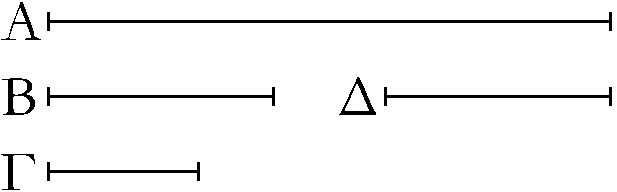
\includegraphics{Book06/fig17g.pdf}}

\gr{>'Εστωσαν τρεῖξ εὐθεῖαι ἀνάλογον αἱ Α, Β, Γ, ὡξ ἡ Α πρὸξ
τὴν Β, ο<ύτωξ ἡ Β πρὸξ τὴν Γ; λέγω, <ότι τὸ ὑπὸ τῶν
Α, Γ περιεχόμενον ὀρθογώνιον >ίσον ἐστὶ τῶ| ἀπὸ τῆξ
Β τετραγώνῳ.}

\gr{Κείσθω τῆ| Β >ίση ἡ Δ.}

\gr{Καὶ ἐπεί ἐστιν ὡξ ἡ Α πρὸξ τὴν Β, ο<ύτωξ
ἡ Β πρὸξ τὴν Γ, >ίση δὲ ἡ Β τῆ| Δ, >έστιν >άρα ὡξ ἡ
Α πρὸξ τὴν Β, ἡ Δ πρὸξ τὴν Γ. ἒαν δὲ τέσσαρεξ εὐθεῖαι
ἀνάλογον >ῶσιν, τὸ ὑπὸ τῶν >άκρων περιεχόμενον
[ὀρθογώνιον] >ίσον ἐστὶ τῶ| ὑπὸ τῶν μέσων
περιεθομένῳ ὀρθογωνίῳ. τὸ >άρα ὑπὸ τῶν Α, Γ >ίσον
ἐστὶ τῶ| ὑπὸ τῶν Β, Δ. ἀλλὰ τὸ ὑπὸ τῶν Β, Δ τὸ
ἀπὸ τῆξ Β ἐστιν; >ίση γὰρ ἡ Β τῆ| Δ; τὸ >άρα ὑπὸ τῶν
Α, Γ περιεχόμενον ὀρθογώνιον >ίσον ἐστὶ τῶ| ἀπὸ τῆξ
Β τετραγώνῳ.}

\gr{Ἀλλὰ δὴ τὸ ὑπὸ τῶν Α, Γ >ίσον >έστω τῶ| ἀπὸ τῆξ Β;
λέγω, <ότι ἐστὶν ὡξ ἡ Α πρὸξ τὴν Β, ο<ύτωξ ἡ Β πρὸξ
τὴν Γ.}

\gr{Τῶν γὰρ α\kern -.7pt  ὐτῶν κατασκευασθέντων, ἐπεὶ τὸ ὑπὸ τῶν Α, Γ
>ίσον ἐστὶ τῶ| ἀπὸ τῆξ Β, ἀλλὰ τὸ ἀπὸ τῆξ Β τὸ ὑπὸ
τῶν Β, Δ ἐστιν; >ίση γὰρ ἡ Β τῆ| Δ; τὸ >άρα ὑπὸ τῶν
Α, Γ >ίσον ἐστὶ τῶ| ὑπὸ τῶν Β, Δ.
ἒαν δὲ τὸ ὑπὸ τῶν >άκρων >ίσον >ῆ| τῶ| ὑπὸ τῶν
μέσων, αἱ τέσσαρεξ εὐθεῖαι ἀνάλογόν εἰσιν. >έστιν >άρα ὡξ
ἡ Α πρὸξ τὴν Β, ο<ύτωξ ἡ Δ πρὸξ τὴν Γ. >ίση δὲ ἡ Β τῆ|
Δ; ὡξ >άρα ἡ Α πρὸξ τὴν Β, ο<ύτωξ ἡ Β πρὸξ τὴν Γ.}

\gr{Ἐὰν >άρα τρεῖξ εὐθεῖαι ἀνάλογον >ῶσιν, τὸ ὑπὸ τῶν >άκρων
περιεχόμενον ὀρθογώνιον >ίσον ἐστὶ τῶ| ἀπὸ τῆξ μέσηξ
τετραγώνῳ; κ>ὰν τὸ ὑπὸ τῶν >άκρων περιεχόμενον ὀρθογώνιον
>ίσον >ῆ| τῶ| ἀπὸ τῆξ μέσηξ τετραγώνῳ, αἱ τρεῖξ εὐθεῖαι
ἀνάλογον >έσονται; <όπερ >έδει δεῖχαι.}}

\ParallelRText{
\begin{center}
{\large Proposition 17}
\end{center}

If three straight-lines are proportional, (then)
the rectangle contained by the (two) outermost is equal to the square
on the middle (one). And if the rectangle contained by the (two) outermost
is equal to the square on the middle (one), (then) the three straight-lines
will be proportional.

% Removed epsf size command
\centerline{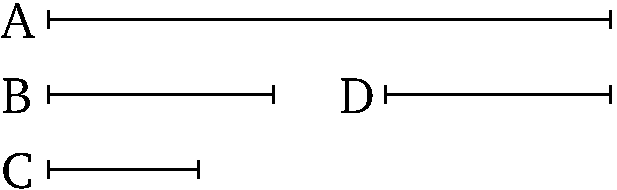
\includegraphics{Book06/fig17e.pdf}}

Let $A$, $B$ and $C$ be three proportional straight-lines, (such that) as $A$ (is) to
$B$, so $B$ (is) to $C$. I say that the rectangle contained by $A$ and $C$ is
equal to the square on $B$.

Let $D$ be made equal to $B$  [Prop.~1.3].

And since as $A$ is to $B$, so $B$ (is) to $C$, and $B$ (is) equal to $D$, thus
as $A$ is to $B$, (so) $D$ (is) to $C$. And if four straight-lines are proportional,
(then) the [rectangle] contained by the (two) outermost is equal
to the rectangle contained by the middle (two) [Prop.~6.16]. Thus, the (rectangle contained)
by $A$ and $C$ is equal to the (rectangle contained) by $B$ and $D$. 
But, the (rectangle contained) by $B$ and $D$ is the (square) on $B$. For
$B$ (is) equal to $D$. Thus, the rectangle contained by $A$ and $C$ is equal
to the square on $B$.

And so, let the (rectangle contained) by $A$ and $C$ be equal to
the (square) on $B$. I say that as $A$ is to $B$, so $B$ (is) to $C$.

For, with the same construction, since the (rectangle contained)
by $A$ and $C$ is equal to the (square) on $B$. But, the (square) on $B$
is the (rectangle contained) by $B$ and $D$. For $B$ (is) equal to $D$.
The (rectangle contained) by $A$ and $C$ is thus equal to the (rectangle
contained) by $B$ and $D$. And if the (rectangle contained) by the (two)
outermost is equal to the (rectangle contained) by the middle (two), (then)
the four straight-lines are proportional [Prop.~6.16]. 
Thus, as $A$ is to $B$, so $D$ (is) to $C$.
And $B$ (is) equal to $D$. Thus, as $A$ (is) to $B$, so $B$ (is) to $C$.

Thus,  if three straight-lines are proportional, (then)
the rectangle contained by the (two) outermost is equal to the square
on the middle (one). And if the rectangle contained by the (two) outermost
is equal to the square on the middle (one), (then) the three straight-lines
will be proportional. (Which is) the very thing it was required to show.}
\end{Parallel}

%%%%%%
% Prop 6.18
%%%%%%
\pdfbookmark[1]{Proposition 6.18}{pdf6.18}
\begin{Parallel}{}{} 
\ParallelLText{
\begin{center}
{\large \ggn{18}.}
\end{center}\vspace*{-7pt}

\gr{Ἀπὸ τῆξ δοθείσηξ  εὐθείαξ τῶ| δοθέντι εὐθυγράμμῳ
<όμοιόν τε καὶ ὁμοίωξ κείμενον εὐθύγραμμον ἀναγράψαι.}

\gr{>'Εστω ἡ μὲν δοθεῖσα εὐθεῖα ἡ ΑΒ, τὸ δὲ δοθὲν εὐθύγραμμ\-ον τὸ ΓΕ;
δεῖ δὴ ἀπὸ τῆξ ΑΒ εὐθείαξ τῶ| ΓΕ εὐθυγράμμῳ <όμοιόν
τε καὶ ὁμοίωξ κείμενον εὐθύγραμμον ἀναγράψαι.}\\

% Removed epsf size command
\centerline{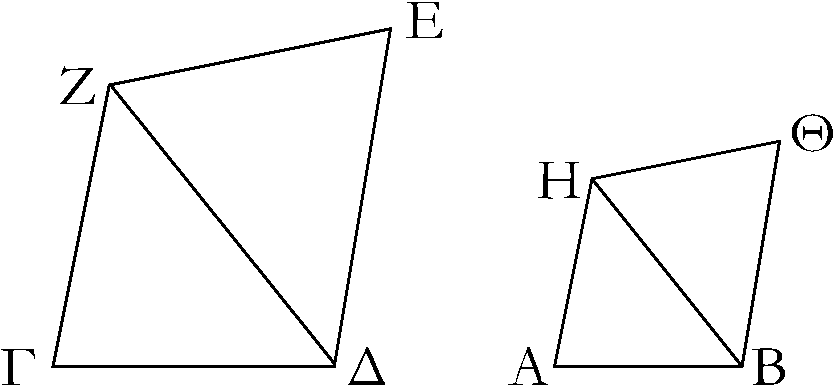
\includegraphics{Book06/fig18g.pdf}}

\gr{Ἐπεζεύθθω ἡ ΔΖ, καὶ συνεστάτω πρὸξ τῆ| ΑΒ εὐθείᾳ καὶ
τοῖξ πρὸξ α\kern -.7pt  ὐτῆ| σημείοιξ τοῖξ Α, Β τῆ| μὲν πρὸξ τῶ| Γ
γωνίᾳ >ίση ἡ ὑπὸ ΗΑΒ, τῆ| δὲ ὑπὸ
ΓΔΖ >ίση ἡ ὑπὸ ΑΒΗ. λοιπὴ >άρα ἡ ὑπὸ ΓΖΔ τῆ| ὑπὸ
ΑΗΒ ἐστιν >ίση; ἰσογώνιον >άρα ἐστὶ τὸ ΖΓΔ τρίγωνον
τῶ| ΗΑΒ τριγώνῳ. ἀνάλογον >άρα ἐστὶν ὡξ ἡ ΖΔ πρὸξ τὴν
ΗΒ, ο<ύτωξ ἡ ΖΓ πρὸξ τὴν ΗΑ, καὶ ἡ ΓΔ πρὸξ τὴν ΑΒ. πάλιν συνεστάτω πρὸξ τῆ| ΒΗ εὐθείᾳ καὶ τοῖξ πρὸξ α\kern -.7pt  ὐτῆ| σημείοιξ
τοῖξ Β, Η τῆ| μὲν ὑπὸ ΔΖΕ γωνίᾳ >ίση ἡ ὑπὸ ΒΗΘ, τῆ|
δὲ ὑπὸ ΖΔΕ >ίση ἡ ὑπὸ ΗΒΘ. λοιπὴ >άρα ἡ πρὸξ
τῶ| Ε λοιπῆ| τῆ| πρὸξ τῶ| Θ ἐστιν >ίση; ἰσογώνιον >άρα
ἐστὶ τὸ ΖΔΕ τρίγωνον τῶ| ΗΘΒ τριγώνῳ; ἀνάλογον
>άρα ἐστὶν ὡξ ἡ ΖΔ πρὸξ τὴν ΗΒ, ο<ύτωξ ἡ
ΖΕ πρὸξ τὴν ΗΘ καὶ ἡ ΕΔ πρὸξ τὴν ΘΒ. ἐδείθθη δὲ καὶ ὡξ ἡ ΖΔ
 πρὸξ τὴν ΗΒ, ο<ύτωξ ἡ ΖΓ πρὸξ τὴν ΗΑ καὶ ἡ ΓΔ πρὸξ
 τὴν
 ΑΒ; καὶ ὡξ >άρα ἡ ΖΓ πρὸξ τὴν ΑΗ, ο<ύτωξ
 <ή τε ΓΔ πρὸξ τὴν ΑΒ καὶ ἡ ΖΕ πρὸξ τὴν ΗΘ καὶ 
 >έτι ἡ ΕΑ πρὸξ τὴν ΘΒ. 
 καὶ ἐπεὶ >ίση ἐστὶν ἡ μὲν ὑπὸ ΓΖΔ γωνία
 τῆ| ὑπὸ ΑΗΒ, ἡ δὲ ὑπὸ ΔΖΕ τῆ| ὑπὸ ΒΗΘ, <όλη
 >άρα ἡ ὑπὸ ΓΖΕ <όλῃ τῆ| ὑπὸ ΑΗΘ ἐστιν >ίση. διὰ τὰ α\kern -.5pt  ὐτὰ
 δὴ καὶ ἡ ὑπὸ ΓΔΕ τῆ| ὑπὸ ΑΒΘ ἐστιν >ίση. >έστι δὲ καὶ
 ἡ μὲν πρὸξ τῶ| Γ τῆ| πρὸξ τῶ| Α >ίση, ἡ δὲ
πρὸξ τῶ| Ε τῆ| πρὸξ τῶ| Θ. ἰσογώνιον >άρα ἐστὶ τὸ ΑΘ τῶ| ΓΕ;
 καὶ τὰξ περὶ τὰξ >ίσαξ γωνίαξ α\kern -.3pt  ὐτῶν πλευρὰξ ἀνάλογον
 >έθει; <όμοιον >άρα ἐστὶ τὸ ΑΘ εὐθύγραμμον τῶ| ΓΕ
 εὐθυγράμμῳ.}
 
 \gr{Ἀπὸ  τῆξ δοθείσηξ  >άρα εὐθείαξ τῆξ ΑΒ τῶ| δοθέντι εὐθυγράμμῳ
τῶ| ΓΕ <όμοιόν τε καὶ ὁμοίωξ κείμενον εὐθύγρα\-μμον ἀναγέγραπται
τὸ ΑΘ;
<όπερ >έδει ποιῆσαι.}}

\ParallelRText{
\begin{center}
{\large Proposition 18}
\end{center}

To describe a rectilinear figure similar, and similarly laid down, to a
given rectilinear figure on a given straight-line.

Let $AB$ be the given straight-line, and $CE$ the given rectilinear figure.
So it is required to describe a rectilinear figure similar, and similarly laid down,   to the rectilinear
figure $CE$ on the straight-line $AB$.

% Removed epsf size command
\centerline{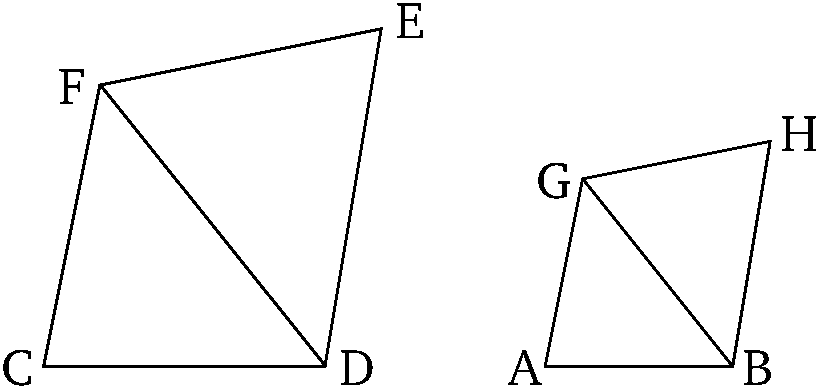
\includegraphics{Book06/fig18e.pdf}}

Let $DF$ be joined, and let $GAB$, equal to the angle at $C$, and $ABG$,
equal to (angle) $CDF$, be constructed  on the straight-line $AB$  
at the points $A$ and $B$ on it (respectively) [Prop.~1.23]. Thus, the
remaining (angle) $CFD$ is equal to $AGB$  [Prop.~1.32].
Thus, triangle $FCD$ is equiangular to triangle $GAB$. Thus, proportionally,
as $FD$ is to $GB$, so $FC$ (is) to $GA$, and $CD$ to $AB$ [Prop.~6.4]. Again, let $BGH$, equal to angle $DFE$,
and $GBH$ equal to (angle) $FDE$, be constructed on the straight-line $BG$  at the points $G$ and
$B$ on it (respectively) [Prop.~1.23]. Thus, the
remaining (angle) at $E$ is equal to the remaining (angle) at $H$  [Prop.~1.32]. Thus, triangle $FDE$ is equiangular to triangle $GHB$.
Thus, proportionally, as $FD$ is to $GB$, so $FE$ (is) to $GH$, and $ED$ to 
$HB$ [Prop.~6.4]. And it was also
shown (that) as $FD$ (is) to $GB$, so $FC$ (is) to $GA$, and $CD$ to $AB$. Thus, also, as $FC$  (is) to $AG$, so  $CD$ (is) to $AB$, and $FE$ to $GH$, and, further, $ED$ to
$HB$. And since angle $CFD$ is equal to $AGB$, and $DFE$ to $BGH$, thus the
whole (angle) $CFE$ is equal to the whole (angle) $AGH$. So, for the same (reasons), (angle) $CDE$ is also equal to $ABH$. And the (angle) at $C$ is also equal to
the (angle) at $A$, and the (angle) at $E$ to the (angle) at $H$. Thus,  (figure) $AH$
is equiangular to $CE$. And (the two figures) have the sides about their equal angles
proportional. Thus, the rectilinear figure $AH$ is similar to the rectilinear figure
$CE$ [Def.~6.1].

Thus, the rectilinear figure $AH$, similar,  and similarly laid down, to the given rectilinear figure
$CE$ has been constructed on the given straight-line
$AB$. (Which is) the very thing it was required to do.}
\end{Parallel}

%%%%%%
% Prop 6.19
%%%%%%
\pdfbookmark[1]{Proposition 6.19}{pdf6.19}
\begin{Parallel}{}{} 
\ParallelLText{
\begin{center}
{\large \ggn{19}.}
\end{center}\vspace*{-7pt}

\gr{Τὰ <όμοια τρίγωνα πρὸξ >άλληλα ἐν διπλασίονι λόγῳ ἐστὶ τῶν
ὁμολόγων πλευρῶν.}

\gr{>'Εστω <όμοια τρίγωνα τὰ ΑΒΓ, ΔΕΖ >ίσην >έθοντα τὴν πρὸξ
τῶ| Β γωνίαν τῆ| πρὸξ τῶ| Ε, ὡξ δὲ τὴν ΑΒ πρὸξ τὴν ΒΓ,
ο<ύτωξ τὴν ΔΕ πρὸξ τὴν ΕΖ, <ώστε ὁμόλογον ε>ῖναι
τὴν ΒΓ τῆ| ΕΖ; λέγω, <ότι τὸ ΑΒΓ τρίγωνον πρὸξ τὸ ΔΕΖ
τρίγωνον διπλασίονα λόγον >έθει >ήπερ ἡ ΒΓ πρὸξ τὴν ΕΖ.}

\gr{Εἰλήφθω γὰρ τῶν ΒΓ, ΕΖ τρίτη ἀνάλογον ἡ ΒΗ, <ώστε
ε>ῖναι ὡξ τὴν ΒΓ πρὸξ τὴν ΕΖ, ο<ύτωξ τὴν ΕΖ πρὸξ τὴν ΒΗ; καὶ
ἐπεζεύθθω ἡ ΑΗ.}

% Removed epsf size command
\centerline{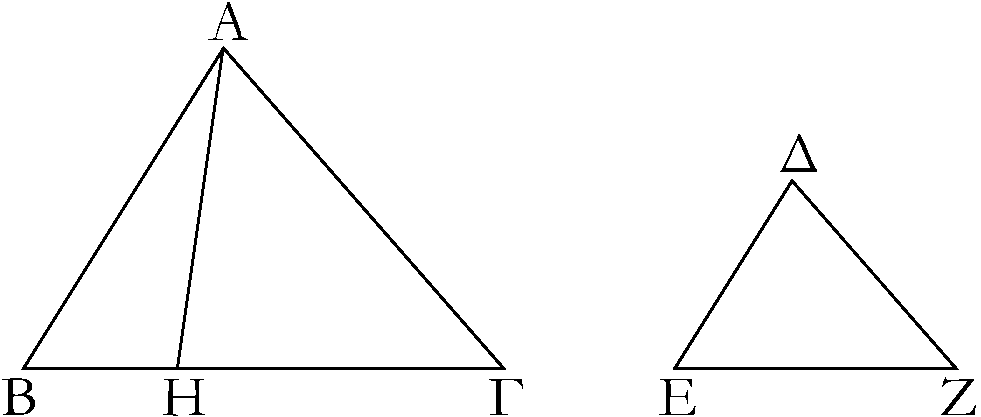
\includegraphics{Book06/fig19g.pdf}}

\gr{Ἐπεὶ ο>ῦν ἐστιν ὡξ ἡ ΑΒ πρὸξ τὴν ΒΓ, ο<ύτωξ
ἡ ΔΕ πρὸξ τὴν ΕΖ, ἐναλλὰχ >άρα ἐστὶν ὡξ ἡ ΑΒ πρὸξ τὴν
ΔΕ, ο<ύτωξ ἡ ΒΓ πρὸξ τὴν ΕΖ. ἀλλ> ὡξ ἡ ΒΓ πρὸξ ΕΖ, ο<ύτωξ
ἐστὶν ἡ ΕΖ πρὸξ ΒΗ. καὶ ὡξ >άρα ἡ ΑΒ πρὸξ ΔΕ, ο<ύτωξ
ἡ ΕΖ πρὸξ ΒΗ; τῶν ΑΒΗ, ΔΕΖ >άρα τριγώνων ἀντιπεπόνθασιν
αἱ πλευραὶ αἱ περὶ τὰξ >ίσαξ γωνάιξ. <ῶν δὲ μίαν μιᾶ|
>ίσην ἐθόντων γωνίαν τριγώνων ἀντιπεπόνθασιν αἱ
πλευραὶ αἱ περὶ τὰξ >ίσαξ γωνάιξ, >ίσα ἐστὶν
ἐκεῖνα. >ίσον >άρα ἐστὶ τὸ ΑΒΗ τρίγωνον τῶ| ΔΕΖ τριγώνῳ.
καὶ ἐπεί ἐστιν ὡξ ἡ ΒΓ πρὸξ τὴν ΕΖ, 
ο<ύτωξ ἡ ΕΖ πρὸξ τὴν ΒΗ, ἒαν δὲ τρεῖξ εὐθεῖαι
ἀνάλογον >ῶσιν, ἡ πρώτη πρὸξ τὴν τρίτην διπλασίονα
λόγον >έθει >ήπερ πρὸξ τὴν δευτέραν, ἡ ΒΓ >άρα πρὸξ τὴν ΒΗ
διπλασίονα λόγον >έθει >ήπερ ἡ ΓΒ πρὸξ τὴν ΕΖ. ὡξ δὲ ἡ
ΓΒ πρὸξ τὴν ΒΗ, ο<ύτωξ τὸ ΑΒΓ τρίγωνον πρὸξ τὸ ΑΒΗ τρίγωνον;
καὶ τὸ ΑΒΓ >άρα τρίγωνον πρὸξ τὸ ΑΒΗ διπλασίονα
λόγον >έθει >ήπερ ἡ ΒΓ πρὸξ τὴν ΕΖ. >ίσον δὲ τὸ ΑΒΗ
τρίγωνον τῶ| ΔΕΖ τριγώνῳ; καὶ τὸ ΑΒΓ >άρα τρίγωνον πρὸξ
τὸ ΔΕΖ τρίγωνον διπλασίονα λόγον >έθει >ήπερ ἡ ΒΓ πρὸξ
τὴν ΕΖ.}

\gr{Τὰ >άρα <όμοια τρίγωνα πρὸξ >άλληλα ἐν διπλασίονι λόγῳ ἐστὶ τῶν
ὁμολόγων πλευρῶν. [<όπερ >έδει δεῖχαι.]}\\~\\

\begin{center}
{\large \gr{Πόρισμα}.}
\end{center}\vspace*{-7pt}

\gr{Ἐκ δὴ τούτου φανερόν, <ότι, ἒαν τρεῖξ εὐθεῖαι
ἀνάλογον >ῶσιν, >έστιν ὡξ ἡ πρώτη πρὸξ τὴν
τρίτην, ο<ύτωξ τὸ ἀπὸ τῆξ πρώτηξ ε>ῖδοξ πρὸξ τὸ ἀπὸ τῆξ
δευτέραξ τὸ <όμοιον καὶ ὁμοίωξ ἀναγραφόμενον. <όπερ
>έδει δεῖχαι.}}

\ParallelRText{
\begin{center}
{\large Proposition 19}
\end{center}

Similar triangles are to one another in the squared$^\dag$
ratio of (their) corresponding sides.

Let $ABC$ and $DEF$ be similar triangles having the angle at $B$ equal to
the (angle)  at $E$, and $AB$  to $BC$, as $DE$ (is) to $EF$, such that
$BC$ corresponds to $EF$. I say that triangle $ABC$ has a
squared ratio to triangle $DEF$ with respect to (that side) $BC$ (has) to $EF$.

For let a third (straight-line), $BG$, be taken (which is)
proportional to $BC$ and $EF$,  so that as $BC$ (is) to $EF$, so $EF$ (is)
to $BG$ [Prop.~6.11]. And let $AG$
be joined.

% Removed epsf size command
\centerline{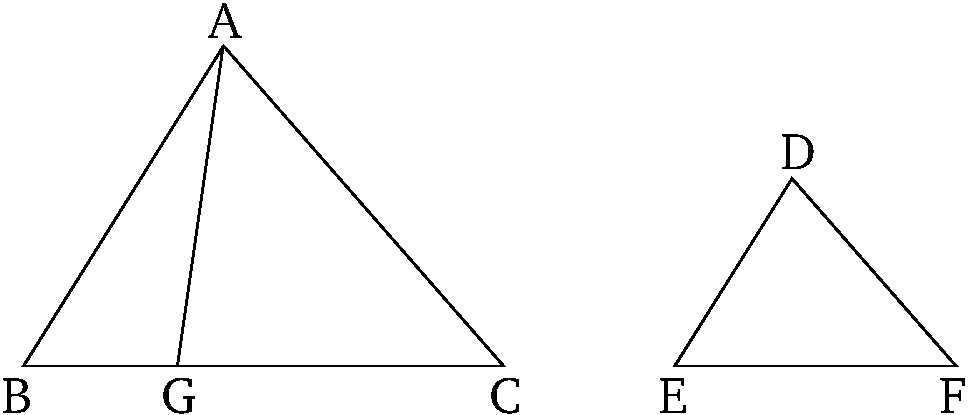
\includegraphics{Book06/fig19e.pdf}}

Therefore, since as $AB$ is to $BC$, so $DE$ (is) to $EF$, thus, alternately, 
as $AB$ is to $DE$, so $BC$ (is) to $EF$ [Prop.~5.16].
But, as $BC$ (is) to $EF$, so $EF$ is to $BG$. And, thus, as $AB$ (is) to $DE$,
so $EF$ (is) to $BG$. Thus, for triangles $ABG$ and $DEF$, the sides
about the equal angles are reciprocally proportional. And those triangles
 having one (angle) equal to one (angle) for which the sides
about the equal angles are reciprocally proportional are equal [Prop.~6.15]. Thus, triangle
$ABG$ is equal to triangle $DEF$. And since as $BC$ (is) to $EF$, so
$EF$ (is) to $BG$, and if three straight-lines are proportional, (then) the
first has a squared ratio to the third with respect to the second  [Def.~5.9],  $BC$ thus has a squared ratio to $BG$ with
respect to  (that) $CB$ (has) to $EF$.  And as $CB$ (is) to
$BG$, so triangle $ABC$ (is) to triangle $ABG$ [Prop.~6.1].  Thus, triangle $ABC$ also has a squared
ratio to (triangle) $ABG$ with respect to (that side) $BC$ (has) to $EF$. And triangle
$ABG$ (is) equal to triangle $DEF$. Thus, triangle $ABC$ also
has a squared ratio to triangle $DEF$ with respect to (that side) $BC$ (has) to $EF$.

Thus, similar triangles are to one another in the squared
ratio of  (their) corresponding sides. [(Which is) the very thing it was required
to show].\\

\begin{center}
{\large Corollary}
\end{center}\vspace*{-7pt}

So it is clear, from this, that if three straight-lines are proportional, (then)
as the first is to the third, so  the figure (described) on the first (is) to the similar,
and similarly described, (figure) on the second. (Which is) the very thing it
was required to show.}
\end{Parallel}
{\footnotesize\noindent$^\dag$ Literally, ``double''.}

%%%%%%
% Prop 6.20
%%%%%%
\pdfbookmark[1]{Proposition 6.20}{pdf6.20}
\begin{Parallel}{}{} 
\ParallelLText{
\begin{center}
{\large \ggn{20}.}
\end{center}\vspace*{-7pt}

\gr{Τὰ <όμοια  πολύγωνα ε>ίξ τε <όμοια τρίγωνα διαιρεῖται καὶ εἰξ >ίσα
τὸ πλῆθοξ καὶ ὁμόλογα τοῖξ <όλοιξ, καὶ τὸ πολύγωνον πρὸξ
τὸ πολύγωνον διπλασίονα λόγον >έθει >ήπερ ἡ ὁμόλογοξ
πλευρὰ πρὸξ τὴν ὁμόλογον πλευράν.}

\gr{>'Εστω <όμοια πολύγωνα τὰ ΑΒΓΔΕ, ΖΗΘΚΛ,
ὁμόλογοξ δὲ >έστω ἡ ΑΒ τῆ| ΖΗ; λέγω, <ότι τὰ ΑΒΓΔΕ,
ΖΗΘΚΛ πολύγωνα ε>ίξ τε <όμοια τρίγωνα διαιρεῖται καὶ εἰξ >ίσα
τὸ πλῆθοξ καὶ ὁμόλογα τοῖξ <όλοιξ, καὶ τὸ ΑΒΓΔΕ πολύγωνον
πρὸξ τὸ ΖΗΘΚΛ πολύγωνον διπλασίονα λόγον >έθει >ήπερ ἡ ΑΒ
πρὸξ τὴν ΖΗ.}\\

% Removed epsf size command
\centerline{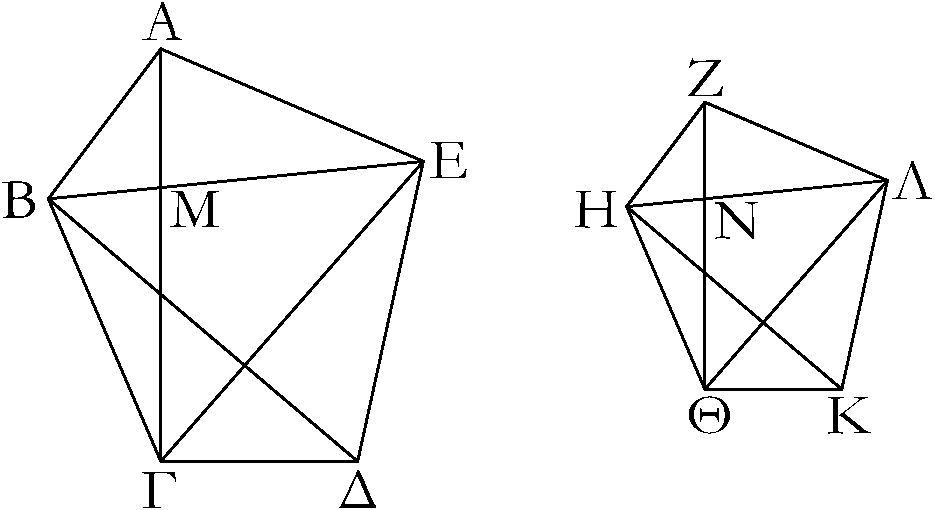
\includegraphics{Book06/fig20g.pdf}}

\gr{Ἐπεζεύθθωσαν αἱ ΒΕ, ΕΓ, ΗΛ, ΛΘ.}

\gr{Καὶ ἐπεὶ <όμοιόν ἐστι τὸ ΑΒΓΔΕ πολύγωνον τῶ| ΖΗΘΚΛ
πολυγώνῳ, >ίση ἐστὶν ἡ ὑπὸ ΒΑΕ γωνία 
τῆ| ὑπὸ ΗΖΛ. καί ἐστιν
ὡξ ἡ ΒΑ πρὸξ ΑΕ, ο<ύτωξ ἡ ΗΖ πρὸξ ΖΛ. ἐπεὶ ο>ῦν δύο
τρίγωνά ἐστι τὰ ΑΒΕ, ΖΗΛ μίαν γωνίαν μιᾶ| γωνίᾳ >ίσην
>έθοντα, περὶ δὲ τὰξ >ίσαξ γωνίαξ τὰξ πλευρὰξ ἀνάλογον,
ἰσογώνιον >άρα ἐστὶ τὸ ΑΒΕ τρίγωνον τῶ| ΖΗΛ τριγώνῳ; <ώστε
καὶ <όμοιον; >ίση >άρα ἐστὶν ἡ ὑπὸ ΑΒΕ γωνία τῆ| ὑπὸ ΖΗΛ.
>έστι δὲ καὶ <όλη ἡ ὑπὸ ΑΒΓ <όλῃ τῆ| ὑπὸ ΖΗΘ >ίση διὰ τὴν
ὁμοιότητα τῶν πολυγώνων; λοιπὴ >άρα ἡ ὑπὸ ΕΒΓ
γωνία τῆ| ὑπὸ ΛΗΘ ἐστιν >ίση. καὶ ἐπεὶ διὰ τὴν ὁμοιότητα
τῶν ΑΒΕ, ΖΗΛ τριγώνων ἐστὶν ὡξ ἡ ΕΒ πρὸξ ΒΑ, ο<ύτωξ
ἡ ΛΗ πρὸξ ΗΖ, 
ἀλλὰ μ\kern -.7pt  ὴν καὶ διὰ τὴν ὁμοιότητα τῶν πολυγώνων
ἐστὶν ὡξ ἡ ΑΒ πρὸξ ΒΓ, ο<ύτωξ ἡ ΖΗ πρὸξ ΗΘ, δι> >ίσου >άρα
ἐστὶν ὡξ ἡ
ΕΒ πρὸξ ΒΓ, ο<ύτωξ ἡ ΛΗ πρὸξ ΗΘ, καὶ περὶ
τὰξ >ίσαξ γωνάιξ τὰξ ὑπὸ ΕΒΓ, ΛΗΘ αἱ πλευραὶ ἀνάλογόν
εἰσιν; ἰσογώνιον >άρα ἐστὶ τὸ ΕΒΓ τρίγωνον τῶ| ΛΗΘ
τριγώνῳ; <ώστε καὶ <όμοιόν ἐστι τὸ ΕΒΓ τρίγωνον τῶ| ΛΗΘ
τριγώνω. διὰ τὰ α\kern -.7pt  ὐτὰ δὴ καὶ τὸ ΕΓΔ τρίγωνον <όμοιόν
ἐστι τῶ| ΛΘΚ τριγώνῳ. τὰ >άρα <όμοια πολύγωνα τὰ ΑΒΓΔΕ, ΖΗΘΚΛ
ε>ίξ τε <όμοια τρίγωνα διή|ρηται καὶ εἰξ >ίσα
τὸ πλῆθοξ.}

\gr{Λέγω, <ότι καὶ ὁμόλογα τοῖξ <όλοιξ, τουτέστιν <ώστε ἀνάλογον
ε>ῖναι τὰ τρίγωνα, καὶ ἡγούμενα μὲν ε>ῖναι τὰ ΑΒΕ, ΕΒΓ, ΕΓΔ, ἑπόμενα δὲ α\kern -.7pt  ὐτῶν τὰ ΖΗΛ, ΛΗΘ, ΛΘΚ, καὶ <ότι τὸ ΑΒΓΔΕ πολύγωνον πρὸξ τὸ ΖΗΘΚΛ πολύγωνον διπλασίονα λόγον >έθει
>ήπερ ἡ ὁμόλογοξ πλευρὰ πρὸξ τὴν ὁμόλογον πλευράν, τουτέστιν
ἡ ΑΒ πρὸξ τὴν ΖΗ.}

\gr{Ἐπεζεύθθωσαν γὰρ αἱ  ΑΓ, ΖΘ. καὶ ἐπεὶ διὰ τὴν ὁμοιότητα τῶν
πολυγώνων >ίση ἐστὶν ἡ ὑπὸ ΑΒΓ γωνία τῆ| ὑπὸ ΖΗΘ, καί ἐστιν ὡξ ἡ ΑΒ πρὸξ ΒΓ, ο<ύτωξ ἡ ΖΗ πρὸξ ΗΘ, ἰσογώνιόν ἐστι
τὸ ΑΒΓ τρίγωνον τῶ| ΖΗΘ τριγώνῳ; >ίση >άρα ἐστὶν ἡ μὲν
ὑπὸ ΒΑΓ γωνία τῆ| ὑπὸ ΗΖΘ, ἡ δὲ ὑπὸ ΒΓΑ
τῆ| ὑπὸ ΗΘΖ. καὶ ἐπεὶ >ίση ἐστὶν ἡ ὑπὸ ΒΑΜ γωνία τῆ| ὑπὸ
ΗΖΝ, >έστι δὲ καὶ ἡ ὑπὸ ΑΒΜ τῆ| ὑπὸ ΖΗΝ >ίση, καὶ λοιπὴ
>άρα ἡ ὑπὸ ΑΜΒ λοιπῆ| τῆ| ὑπὸ ΖΝΗ >ίση ἐστίν; ἰσογώνιον
>άρα ἐστὶ τὸ ΑΒΜ τρίγωνον τῶ| ΖΗΝ τριγώνῳ. ὁμοίωξ δὴ δεῖχομεν, <ότι καὶ τὸ ΒΜΓ τρίγωνον ἰσογώνιόν ἐστι τῶ| ΗΝΘ
τριγώνῳ. ἀνάλογον >άρα ἐστίν, ὡξ μὲν ἡ ΑΜ πρὸξ ΜΒ, ο<ύτωξ ἡ ΖΝ πρὸξ ΝΗ, ὡξ δὲ ἡ ΒΜ πρὸξ ΜΓ, ο<ύτωξ ἡ ΗΝ πρὸξ ΝΘ; 
<ώστε καὶ δι> >ίσου, ὡξ ἡ ΑΜ πρὸξ ΜΓ, ο<ύτωξ ἡ ΖΝ πρὸξ ΝΘ.
ἀλλ> ὡξ ἡ ΑΜ πρὸξ ΜΓ, ο<ύτωξ τὸ ΑΒΜ [τρίγωνον] πρὸξ τὸ
ΜΒΓ, καὶ τὸ ΑΜΕ πρὸξ τὸ  ΕΜΓ; πρὸξ >άλληλα γάρ εἰσιν
ὡξ αἱ βάσειξ. καὶ ὡξ >άρα <ὲν τῶν ἡγουμένων πρὸξ <ὲν
τῶν ἑπόμενων, ο<ύτωξ <άπαντα τὰ ἡγούμενα πρὸξ <άπαντα
τὰ ἑπόμενα; ὡξ >άρα τὸ ΑΜΒ τρίγωνον πρὸξ τὸ ΒΜΓ, ο<ύτωξ τὸ
ΑΒΕ πρὸξ τὸ ΓΒΕ. αλλ> ὡξ τὸ ΑΜΒ πρὸξ τὸ ΒΜΓ, ο<ύτωξ
ἡ ΑΜ πρὸξ ΜΓ; καὶ ὡξ >άρα ἡ ΑΜ πρὸξ ΜΓ, ο<ύτωξ τὸ ΑΒΕ
τρίγωνον πρὸξ τὸ ΕΒΓ τρίγωνον. διὰ τὰ α\kern -.7pt  ὐτὰ δὴ καὶ ὡξ ἡ ΖΝ πρὸξ
ΝΘ, ο<ύτωξ τὸ ΖΗΛ τρίγωνον πρὸξ τὸ ΗΛΘ τρίγωνον. καί ἐστιν ὡξ
ἡ ΑΜ πρὸξ ΜΓ, ο<ύτωξ ἡ ΖΝ πρὸξ ΝΘ; καὶ ὡξ >άρα τὸ ΑΒΕ τρίγωνον 
πρὸξ τὸ ΒΕΓ τρίγωνον, ο<ύτωξ τὸ ΖΗΛ τρίγωνον πρὸξ τὸ ΗΛΘ τρίγωνον,
καὶ ἐναλλὰχ ὡξ τὸ ΑΒΕ τρίγωνον πρὸξ τὸ ΖΗΛ τρίγωνον, ο<ύτωξ
τὸ ΒΕΓ τρίγωνον πρὸξ τὸ ΗΛΘ τρίγωνον. ὁμοίωξ δὴ δείχομεν
ἐπιζευθθεισῶν τῶν ΒΔ, ΗΚ, <ότι καὶ ὡξ τὸ ΒΕΓ τρίγωνον πρὸξ
τὸ ΛΗΘ τρίγωνον, ο<ύτωξ τὸ ΕΓΔ τρίγωνον πρὸξ τὸ ΛΘΚ τρίγωνον.
καὶ ἐπεί ἐστιν ὡξ τὸ ΑΒΕ τρίγωνον πρὸξ τὸ ΖΗΛ τρίγωνον,
ο<ύτωξ τὸ ΕΒΓ πρὸξ τὸ ΛΗΘ, καὶ >έτι τὸ ΕΓΔ πρὸξ τὸ ΛΘΚ,
καὶ ὡξ >άρα <ὲν τῶν ἡγουμένων πρὸξ <ὲν τῶν ἑπομένων, ο<ύτωξ <άπαντα τὰ ἡγούμενα πρὸξ <άπαντα τὰ ἑπόμενα; >έστιν
>άρα ὡξ τὸ ΑΒΕ τρίγωνον πρὸξ τὸ ΖΗΛ τρίγωνον, ο<ύτωξ 
τὸ ΑΒΓΔΕ πολύγωνον πρὸξ τὸ ΖΗΘΚΛ πολύγωνον. ἀλλὰ τὸ
ΑΒΕ τρίγωνον πρὸξ  τὸ ΖΗΛ τρίγωνον διπλασίονα λόγον >έθει >ήπερ
ἡ ΑΒ ὁμόλογοξ πλευρὰ πρὸξ τὴν ΖΗ ὁμόλογον πλευράν; τὰ γὰρ
<όμοια τρίγωνα ἐν διπλασίονι λόγῳ ἐστὶ τῶν ὁμολόγων πλευρῶν.
καὶ τὸ ΑΒΓΔΕ >άρα πολύγωνον πρὸξ τὸ ΖΗΘΚΛ
πολύγωνον διπλασίονα λόγον >έθει >ήπερ ἡ ΑΒ ὁμόλογοξ
πλευρὰ πρὸξ τὴν ΖΗ ὁμόλογον πλευράν.}

\gr{Τὰ >άρα <όμοια  πολύγωνα ε>ίξ τε <όμοια τρίγωνα διαιρεῖται καὶ εἰξ >ίσα
τὸ πλῆθοξ καὶ ὁμόλογα τοῖξ <όλοιξ, καὶ τὸ πολύγωνον πρὸξ
τὸ πολύγωνον διπλασίονα λόγον >έθει >ήπερ ἡ ὁμόλογοξ
πλευρὰ πρὸξ τὴν ὁμόλογον πλευράν  [<όπερ >έδει δεῖχαι].}\\~\\~\\~\\~\\

\begin{center}
{\large \gr{Πόρισμα}.}
\end{center}\vspace*{-7pt}

\gr{Ὡσα\kern -.7pt  ύτωξ δὲ καὶ ἐπὶ τῶν [ὁμοίων] τετραπλεύρων δειθθή\-σεται, 
<ότι ἐν διπλασίονι λόγῳ εἰσὶ τῶν ὁμολόγων πλευρῶν.
ἐδείθθη δὲ καὶ ἐπὶ τῶν τριγώνων; <ώστε καὶ καθόλου τὰ <όμοια
εὐθύγραμμα σθήματα πρὸξ >άλληλα ἐν διπλασίονι λόγῳ εἰσὶ τῶν
ὁμολόγων πλευρῶν. <όπερ >έδει δεῖχαι.}}

\ParallelRText{
\begin{center}
{\large Proposition 20}
\end{center}

Similar polygons can be divided into equal
numbers of similar
triangles corresponding (in proportion) to the wholes, and one
polygon has to the (other) polygon a squared ratio with respect to
(that) a corresponding side (has) to a corresponding side.

Let $ABCDE$ and $FGHKL$ be similar polygons, and let $AB$ correspond to
$FG$. I say that polygons $ABCDE$ and $FGHKL$ can be divided into equal numbers of similar triangles corresponding (in proportion) to the wholes,
and (that) polygon $ABCDE$ has a squared ratio to polygon
$FGHKL$ with respect to that $AB$ (has) to $FG$.

% Removed epsf size command
\centerline{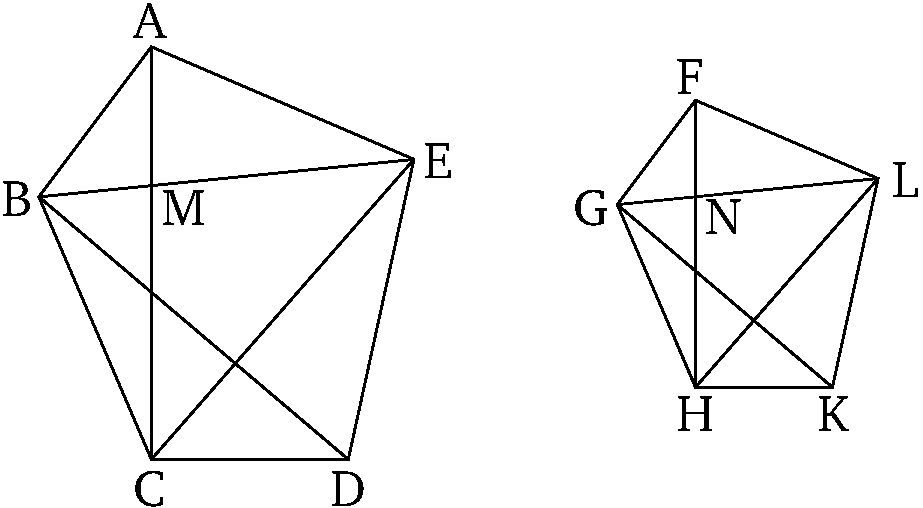
\includegraphics{Book06/fig20e.pdf}}

Let $BE$, $EC$, $GL$, and $LH$ be joined.

And since polygon $ABCDE$ is similar to polygon $FGHKL$, angle
$BAE$ is equal to angle $GFL$,
and as $BA$ is to $AE$, so $GF$ (is) to $FL$ [Def.~6.1].
Therefore, since $ABE$ and $FGL$ are two triangles having one angle equal
to one angle  and the sides about the equal angles proportional, triangle
$ABE$ is thus equiangular to triangle $FGL$ [Prop.~6.6]. Hence, (they are) also similar
 [Prop.~6.4, Def.~6.1]. Thus, angle $ABE$ is equal to
(angle) $FGL$.  And the whole (angle) $ABC$ is equal to the whole (angle)
$FGH$, on  account of the similarity of the polygons. Thus, the remaining
angle $EBC$ is equal to $LGH$. And since, on account of the similarity of
triangles $ABE$ and $FGL$, as $EB$ is to $BA$, so $LG$ (is) to $GF$, but 
also, on account of the similarity of the polygons, as $AB$ is to $BC$, so
$FG$ (is) to $GH$, thus, via equality, as $EB$ is to $BC$, so $LG$ (is) to $GH$ [Prop.~5.22], and the sides about the
equal angles, $EBC$ and $LGH$, are  proportional. Thus, triangle
$EBC$ is equiangular to triangle $LGH$ [Prop.~6.6]. Hence, triangle $EBC$ is also
similar to triangle $LGH$  [Prop.~6.4, Def.~6.1]. So, for the same (reasons), triangle
$ECD$ is also similar to triangle $LHK$. Thus, the similar
polygons $ABCDE$ and $FGHKL$ have been divided into
equal numbers of similar triangles.

I also say that (the triangles) correspond (in proportion) to the wholes.
That is to say,  the triangles are proportional:  $ABE$, $EBC$, and
$ECD$ are the leading (magnitudes), and their (associated) following (magnitudes are) 
$FGL$, $LGH$, and $LHK$ (respectively). (I) also (say) that polygon
$ABCDE$ has a squared ratio to polygon $FGHKL$ with respect to
(that) a corresponding side (has) to a corresponding side---that is to
say, (side) $AB$ to $FG$.

For let $AC$ and $FH$ be joined. And since angle $ABC$ is
equal to $FGH$,  and
as $AB$ is to $BC$, so $FG$ (is) to $GH$, on account of the similarity of the polygons,  triangle $ABC$ is equiangular to triangle
$FGH$ [Prop.~6.6]. Thus, angle $BAC$ is equal 
to $GFH$, and (angle) $BCA$ to $GHF$. And since angle $BAM$ is equal to 
$GFN$, and (angle) $ABM$ is also equal to $FGN$ (see earlier), the remaining (angle) $AMB$ is
thus also equal to the remaining (angle) $FNG$  [Prop.~1.32]. 
Thus, triangle $ABM$ is equiangular to triangle $FGN$. So, similarly, we can
show that triangle $BMC$ is also equiangular to triangle $GNH$. Thus, proportionally,
as $AM$ is to $MB$, so $FN$ (is) to $NG$, and as $BM$ (is) to $MC$, so $GN$ (is) to
$NH$ [Prop.~6.4]. Hence, also, via equality,
as $AM$ (is) to $MC$, so $FN$ (is) to $NH$ 
[Prop.~5.22]. But, as $AM$ (is) to $MC$,
so [triangle] $ABM$ is to $MBC$, and $AME$ to $EMC$. For they are to one another
 as their bases  [Prop.~6.1]. And as one
 of the leading (magnitudes) is to one of the following (magnitudes), so
    (the sum of) all the leading (magnitudes) is to (the sum of) all the following (magnitudes)
[Prop.~5.12]. Thus, as triangle $AMB$
 (is) to $BMC$, so (triangle) $ABE$ (is) to $CBE$. But, as (triangle) $AMB$ (is) to
 $BMC$, so $AM$ (is) to $MC$. Thus, also, as $AM$ (is) to $MC$, so 
triangle $ABE$
 (is) to triangle $EBC$. And so, for the same (reasons), as $FN$ (is) to $NH$,
 so triangle $FGL$  (is) to triangle $GLH$. And as $AM$ is to $MC$, so $FN$ (is) to
 $NH$. Thus, also, as triangle $ABE$ (is) to triangle $BEC$, so triangle $FGL$
 (is) to triangle $GLH$, and, alternately, as triangle $ABE$ (is) to triangle
 $FGL$, so triangle $BEC$ (is) to triangle $GLH$  [Prop.~5.16]. So, similarly, we can also show, by
 joining $BD$ and $GK$, (that)  as triangle $BEC$ (is) to triangle $LGH$,
 so triangle $ECD$ (is) to triangle $LHK$. And since as triangle $ABE$ is
 to triangle $FGL$, so (triangle) $EBC$ (is) to $LGH$, and, further, (triangle)
 $ECD$ to $LHK$, and also as one of the leading (magnitudes is) to one
 of the following, so (the sum of) all the leading (magnitudes is) to (the sum of) all the
 following [Prop.~5.12], thus as triangle
 $ABE$ is to triangle $FGL$, so polygon $ABCDE$ (is) to polygon
 $FGHKL$. But, triangle $ABE$ has a squared ratio to triangle $FGL$ with
 respect to (that) the corresponding side $AB$ (has) to the corresponding side
 $FG$. For, similar triangles are in the squared ratio of corresponding sides 
[Prop.~6.14]. Thus, polygon
$ABCDE$ also has a squared ratio to polygon $FGHKL$ with respect to
(that) the corresponding side $AB$ (has) to the corresponding side
$FG$.

Thus, similar polygons can be divided into equal
numbers of similar
triangles corresponding (in proportion) to the wholes, and one
polygon has to the (other) polygon a squared ratio with respect to
(that) a corresponding side (has) to a corresponding side. [(Which is) the
very thing it was required to show].\\

\begin{center}
{\large Corollary}
\end{center}\vspace*{-7pt}

And, in the same manner, it can also be shown for [similar] quadrilaterals,
(that) they are in the squared ratio of (their) corresponding sides. And it was also
shown for triangles. Hence, in general, similar rectilinear figures are also to one
another in the squared ratio of (their) corresponding sides. (Which is) the
very thing it was required to show.\\}
\end{Parallel}

%%%%%%
% Prop 6.21
%%%%%%
\pdfbookmark[1]{Proposition 6.21}{pdf6.21}
\begin{Parallel}{}{} 
\ParallelLText{
\begin{center}
{\large \ggn{21}.}
\end{center}\vspace*{-7pt}

\gr{Τὰ τῶ| α\kern -.7pt  ὐτῶ| εὐθυγράμμῳ <όμοια καὶ ἀλλήλοιξ ἐστὶν <όμοια.}\\

% Removed epsf size command
\centerline{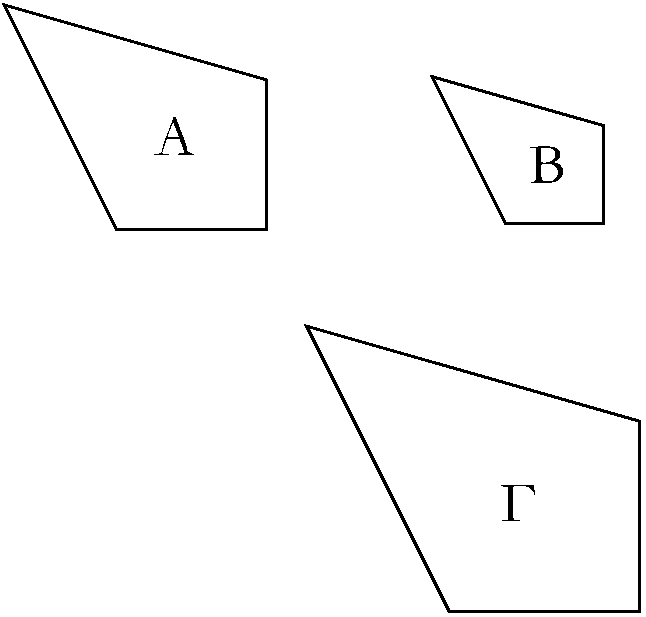
\includegraphics{Book06/fig21g.pdf}}

\gr{>'Εστω γὰρ ἑκάτερον τῶν Α, Β εὐθυγράμμων τῶ| Γ <όμοιον;
λέγω, <ότι καὶ τὸ Α τῶ| Β ἐστιν <όμοιον.}

\gr{Ἐπεὶ γὰρ <όμοιόν ἐστι τὸ Α τῶ| Γ, ἰσογώνιόν τέ ἐστιν
α\kern -.7pt  ὐτῶ| καὶ τὰξ περὶ τὰξ >ίσαξ γωνίαξ πλευρὰξ ἀνάλογον
>έθει. πάλιν, ἐπεὶ <όμοιόν ἐστι τὸ Β τῶ| Γ, ἰσογώνιόν
τέ ἐστιν α\kern -.7pt  ὐτῶ| καὶ τὰξ περὶ τὰξ >ίσαξ γωνίαξ πλευρὰξ ἀνάλογον
>έθει. ἑκάτερον >άρα τῶν Α, Β τῶ| Γ ἰσογώνιόν τέ ἐστι
καὶ τὰξ περὶ τὰξ >ίσαξ γωνίαξ πλευρὰξ ἀνάλογον >έθει [<ώστε
καὶ τὸ Α τῶ| Β ἰσογώνιόν τέ ἐστι καὶ τὰξ περὶ τὰξ 
>ίσαξ γωνίαξ πλευρὰξ ἀνάλογον >έθει]. <όμοιον >άρα ἐστὶ
τὸ Α τῶ| Β; <όπερ >έδει δεῖχαι.}}

\ParallelRText{
\begin{center}
{\large Proposition 21}
\end{center}

(Rectilinear figures) similar to the same rectilinear
figure are also similar to one another.

% Removed epsf size command
\centerline{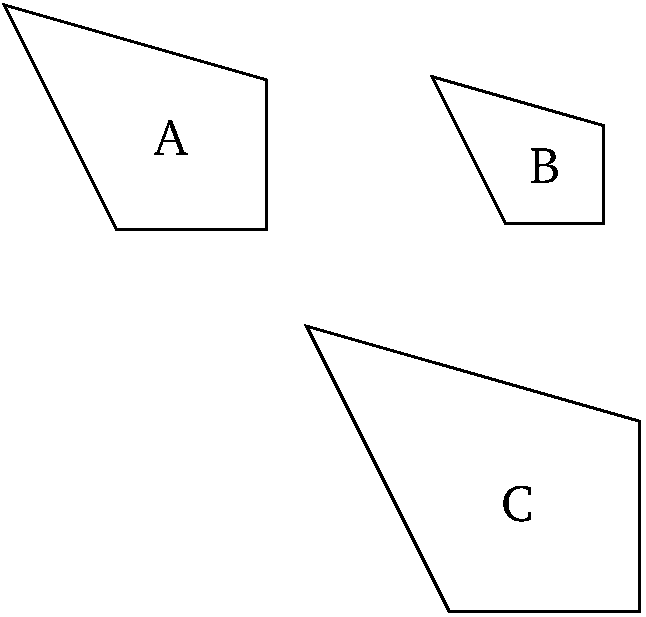
\includegraphics{Book06/fig21e.pdf}}

Let each of the rectilinear figures $A$ and $B$ be similar to (the rectilinear figure)
$C$.  I say that $A$ is also similar to $B$.

For since $A$ is similar to $C$, ($A$) is equiangular to ($C$), and has the sides about
the equal angles proportional [Def.~6.1].
Again, since $B$ is similar to $C$, ($B$) is equiangular to ($C$), and has the sides about the equal angles proportional [Def.~6.1].
Thus, $A$ and $B$ are each equiangular to $C$, and have the sides about the
equal angles proportional [hence, $A$ is also equiangular to $B$, and has the sides
about the equal angles proportional]. Thus, $A$ is similar to $B$ [Def.~6.1]. (Which is) the very thing it was required
to show.}
\end{Parallel}

%%%%%%
% Prop 6.22
%%%%%%
\pdfbookmark[1]{Proposition 6.22}{pdf6.22}
\begin{Parallel}{}{} 
\ParallelLText{
\begin{center}
{\large \ggn{22}.}
\end{center}\vspace*{-7pt}

\gr{Ἐὰν τέσσαρεξ εὐθεῖαι ἀνάλογον >ῶσιν, καὶ τὰ ἀπ> α\kern -.7pt  ὐτῶν
εὐθύγραμμα <όμοιά τε καὶ ὁμοίωξ ἀναγεγραμμένα ἀνάλογον
>έσται; κ>ὰν τὰ ἀπ> α\kern -.7pt  ὐτῶν εὐθύγραμμα <όμοιά τε καὶ ὁμοίωξ
ἀναγεγραμμένα ἀνάλογον >ῆ|, καὶ α\kern -.5pt  ὐτὰι αἱ εὐθεῖαι ἀνάλογον
>έσονται.}

\gr{>'Εστωσαν τέσσαρεξ εὐθεῖαι ἀνάλογον αἱ ΑΒ, ΓΔ, ΕΖ, ΗΘ, ὡξ ἡ ΑΒ
πρὸξ τὴν ΓΔ, ο<ύτωξ ἡ ΕΖ πρὸξ τὴν ΗΘ, καὶ ἀναγεγράφθωσαν
ἀπὸ μὲν τῶν ΑΒ, ΓΔ <όμοιά τε καὶ ὁμοίωξ κείμενα εὐθύγραμμα
τὰ ΚΑΒ, ΛΓΔ, ἀπὸ δὲ τῶν ΕΖ, ΗΘ <όμοιά τε καὶ ὁμοίωξ
κείμενα εὐθύγραμμα τὰ ΜΖ, ΝΘ; λέγω, <ότι  ἐστὶν ὡξ τὸ 
ΚΑΒ πρὸξ τὸ ΛΓΔ, ο<ύτωξ τὸ ΜΖ πρὸξ τὸ ΝΘ.}

\gr{Εἰλήφθω γὰρ τῶν μὲν ΑΒ, ΓΔ τρίτη ἀνάλογον ἡ Χ, τῶν δὲ
ΕΖ, ΗΘ τρίτη ἀνάλογον ἡ Ο. καὶ ἐπεί ἐστιν ὡξ μὲν ἡ ΑΒ
πρὸξ τὴν ΓΔ, ο<ύτωξ ἡ ΕΖ πρὸξ τὴν ΗΘ, ὡξ δὲ ἡ ΓΔ πρὸξ τὴν
 Χ, ο<ύτωξ ἡ ΗΘ πρὸξ τὴν Ο, δι> >ίσου >άρα ἐστὶν
ὡξ ἡ ΑΒ πρὸξ τὴν Χ, ο<ύτωξ ἡ ΕΖ πρὸξ τὴν Ο. ἀλλ>
ὡξ μὲν ἡ ΑΒ πρὸξ τὴν Χ, ο<ύτωξ [καὶ] τὸ ΚΑΒ πρὸξ τὸ
ΛΓΔ, ὡξ δὲ ἡ ΕΖ πρὸξ τὴν Ο, ο<ύτωξ τὸ ΜΖ πρὸξ τὸ ΝΘ;
καὶ ὡξ >άρα τὸ ΚΑΒ πρὸξ τὸ ΛΓΔ, ο<ύτωξ τὸ ΜΖ πρὸξ τὸ
ΝΘ.}

\gr{Ἀλλὰ δὴ >έστω ὡξ τὸ ΚΑΒ πρὸξ τὸ ΛΓΔ, ο<ύτωξ
τὸ ΜΖ πρὸξ τὸ ΝΘ; λέγω,  <ότι ἐστὶ καὶ ὡξ ἡ ΑΒ πρὸξ τὴν
ΓΔ, ο<ύτωξ ἡ ΕΖ πρὸξ  τὴν ΗΘ. εἰ γὰρ μ\kern -.7pt  ή ἐστιν, ὡξ ἡ ΑΒ
πρὸξ τὴν ΓΔ, ο<ύτωξ ἡ ΕΖ πρὸξ τὴν ΗΘ, >έστω ὡξ ἡ
ΑΒ πρὸξ τὴν ΓΔ, ο<ύτωξ ἡ ΕΖ πρὸξ τὴν ΠΡ, καὶ ἀναγεγράφθω
ἀπὸ τῆξ ΠΡ ὁποτέρῳ τῶν ΜΖ, ΝΘ <όμοιόν τε καὶ 
ὁμοίωξ κείμενον εὐθύγραμμον τὸ ΣΡ.}

% Removed epsf size command
\centerline{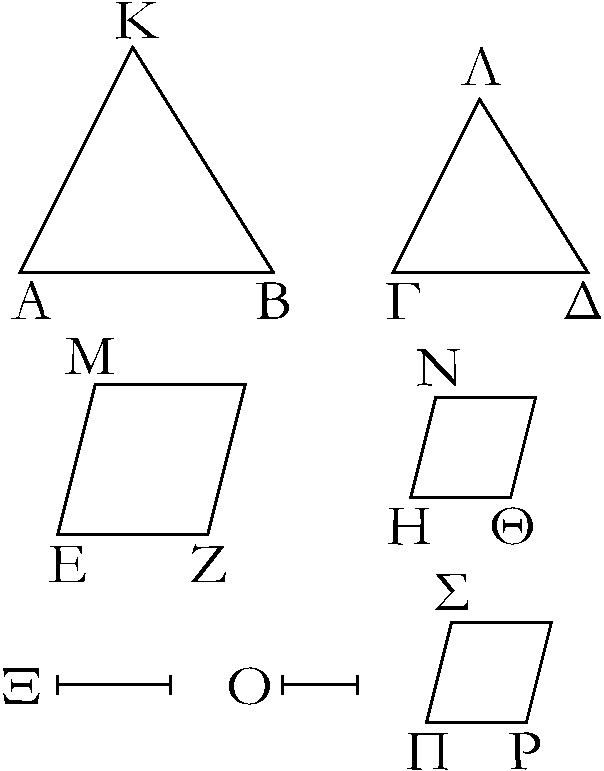
\includegraphics{Book06/fig22g.pdf}}

\gr{Ἐπεὶ ο>ῦν ἐστιν ὡξ ἡ ΑΒ πρὸξ τὴν ΓΔ, ο<ύτωξ ἡ
ΕΖ πρὸξ τὴν ΠΡ, καὶ ἀναγέγραπται ἀπὸ μὲν τῶν ΑΒ, ΓΔ
<όμοιά τε καὶ ὁμοίωξ κείμενα τὰ ΚΑΒ,
ΛΓΔ, ἀπὸ δὲ τῶν ΕΖ, ΠΡ <όμοιά τε καὶ ὁμοίωξ
κείμενα τὰ ΜΖ, ΣΡ, >έστιν >άρα ὡξ τὸ ΚΑΒ πρὸξ τὸ ΛΓΔ,
ο<ύτωξ τὸ ΜΖ πρὸξ τὸ ΣΡ. ὑπόκειται δὲ καὶ ὡξ τὸ ΚΑΒ
πρὸξ τὸ ΛΓΔ, ο<ύτωξ τὸ ΜΖ πρὸξ τὸ ΝΘ; καὶ ὡξ >άρα τὸ ΜΖ
πρὸξ τὸ ΣΡ, ο<ύτωξ τὸ ΜΖ πρὸξ τὸ ΝΘ. τὸ ΜΖ >άρα πρὸξ ἑκάτερον
τῶν ΝΘ, ΣΡ τὸν α\kern -.7pt  ὐτὸν >έθει λόγον; >ίσον >άρα ἐστὶ τὸ ΝΘ τῶ|
ΣΡ. >έστι δὲ α\kern -.7pt  ὐτῶ| καὶ <όμοιον καὶ ὁμοίωξ κείμενον; >ίση >άρα
ἡ ΗΘ τῆ| ΠΡ. καὶ ἐπεί ἐστιν ὡξ ἡ ΑΒ πρὸξ τὴν
ΓΔ, ο<ύτωξ ἡ ΕΖ πρὸξ τὴν ΠΡ, >ίση δὲ ἡ ΠΡ τῆ| ΗΘ, >έστιν
>άρα ὡξ ἡ ΑΒ πρὸξ τὴν ΓΔ, ο<ύτωξ ἡ ΕΖ
πρὸξ τὴν ΗΘ.}

\gr{Ἐὰν >άρα τέσσαρεξ εὐθεῖαι ἀνάλογον >ῶσιν, καὶ τὰ ἀπ> α\kern -.7pt  ὐτῶν
εὐθύγραμμα <όμοιά τε καὶ ὁμοίωξ ἀναγεγραμμένα ἀνάλογον
>έσται; κ>ὰν τὰ ἀπ> α\kern -.7pt  ὐτῶν εὐθύγραμμα <όμοιά τε καὶ ὁμοίωξ
ἀναγεγραμμένα ἀνάλογον >ῆ|, καὶ α\kern -.5pt  ὐτὰι αἱ εὐθεῖαι ἀνάλογον
>έσονται; <όπερ >έδει δεῖχαι.}}

\ParallelRText{
\begin{center}
{\large Proposition 22}
\end{center}

If four straight-lines are proportional, (then)
similar, and similarly described, rectilinear figures (drawn) on them will also
be proportional. And if similar, and similarly described, rectilinear figures (drawn) on them are proportional, (then) the  straight-lines themselves will also be proportional.

Let $AB$, $CD$, $EF$, and $GH$ be four proportional straight-lines, (such
that) as $AB$ (is) to $CD$, so $EF$ (is) to $GH$. And  let the similar, and similarly
laid out, rectilinear figures $KAB$ and $LCD$ be described on
$AB$ and $CD$ (respectively), and the similar, and similarly
laid out, rectilinear figures $MF$ and $NH$ on $EF$ and $GH$ (respectively). 
I say that as $KAB$ is to $LCD$, so $MF$ (is) to $NH$.

For let a third (straight-line) $O$ be taken (which is) proportional to
$AB$ and $CD$, and a third (straight-line) $P$ proportional to $EF$ and $GH$
[Prop.~6.11]. And since as $AB$ is to
$CD$, so $EF$ (is) to $GH$, and as $CD$ (is) to $O$, so $GH$ (is) to $P$, thus, via equality,
as $AB$ is to $O$, so $EF$ (is) to $P$ [Prop.~5.22].
But, as $AB$ (is) to $O$, so [also] $KAB$ (is)  to $LCD$, and as $EF$ (is) to $P$,
so $MF$ (is) to $NH$ [Prop.~5.19~corr.].
And, thus, as $KAB$ (is) to $LCD$, so $MF$ (is) to $NH$.

And so let $KAB$ be to $LCD$, as $MF$ (is) to $NH$. I say also that as
$AB$ is to $CD$, so $EF$ (is) to $GH$. For if as $AB$ is to $CD$, so $EF$ (is) not to $GH$, 
let $AB$ be to $CD$, as $EF$ (is) to $QR$ [Prop.~6.12]. And let the rectilinear figure $SR$, similar, and similarly laid down, to either  of $MF$ or $NH$, be described on
$QR$  [Props.~6.18, 6.21].

% Removed epsf size command
\centerline{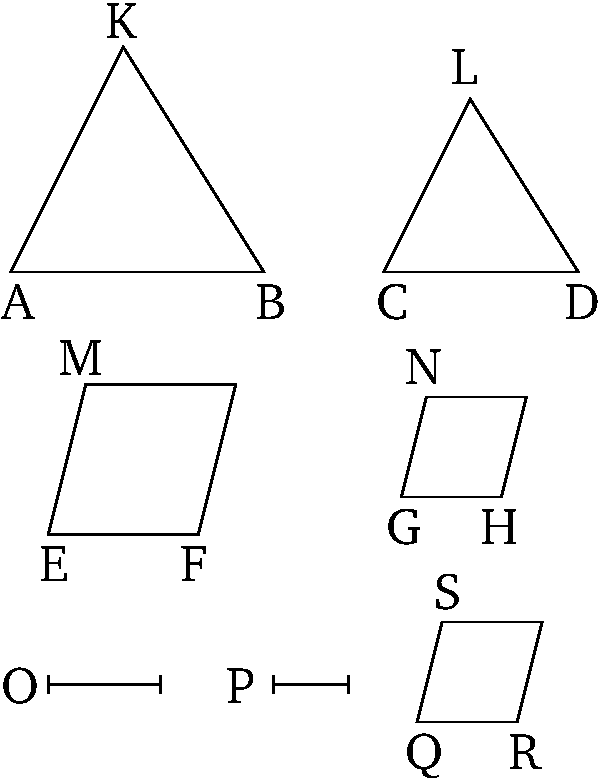
\includegraphics{Book06/fig22e.pdf}}

Therefore, since as $AB$ is to $CD$, so $EF$ (is) to $QR$, and the similar, and
similarly laid out, (rectilinear figures) $KAB$ and $LCD$ have been described
on $AB$  and $CD$ (respectively), and the similar, and similarly laid out, (rectilinear figures) $MF$ and $SR$ on $EF$ and $QR$ (respectively), thus
as $KAB$ is to $LCD$, so $MF$ (is) to $SR$  (see above). And it was also assumed
that as $KAB$ (is) to $LCD$, so $MF$ (is) to $NH$. Thus, also, as $MF$ (is) to $SR$,
so $MF$ (is) to $NH$ [Prop.~5.11]. Thus, $MF$ has the same ratio to each of $NH$ and $SR$. 
Thus, $NH$ is equal to $SR$ [Prop.~5.9].
And it is also similar, and similarly laid out, to it. Thus,  $GH$ (is) equal to $QR$.$^\dag$
And since $AB$ is to $CD$, as $EF$ (is) to $QR$, and $QR$ (is) equal to $GH$, thus
as $AB$ is to $CD$, so $EF$ (is) to $GH$.

Thus, if four straight-lines are proportional, (then)
similar, and similarly described, rectilinear figures (drawn) on them will also
be proportional. And if similar, and similarly described, rectilinear figures (drawn) on them are proportional, (then) the  straight-lines themselves will also be proportional. (Which is) the very thing it was required to show.}
\end{Parallel}
{\footnotesize \noindent$^\dag$ Here, Euclid assumes, without proof, that
if two similar figures are equal then any pair of corresponding sides is also
equal.}

%%%%%%
% Prop 6.23
%%%%%%
\pdfbookmark[1]{Proposition 6.23}{pdf6.23}
\begin{Parallel}{}{} 
\ParallelLText{
\begin{center}
{\large \ggn{23}.}
\end{center}\vspace*{-7pt}

\gr{Τὰ ἰσογώνια παραλληλόγραμμα πρὸξ >άλληλα λόγον >έθει τὸν
συγκείμενον ἐκ τῶν πλευρῶν.}

\gr{>'Εστω ἰσογώνια παραλληλόγραμμα τὰ ΑΓ, ΓΖ >ίσην >έθοντα τὴν
ὑπὸ ΒΓΔ γωνίαν τῆ| ὑπὸ ΕΓΗ; λέγω, <ότι τὸ ΑΓ παραλληλόγραμμον
πρὸξ τὸ ΓΖ παραλληλόγραμμον λόγον >έθει τὸν συγκείμενον
ἐκ τῶν πλευρῶν.}

% Removed epsf size command
\centerline{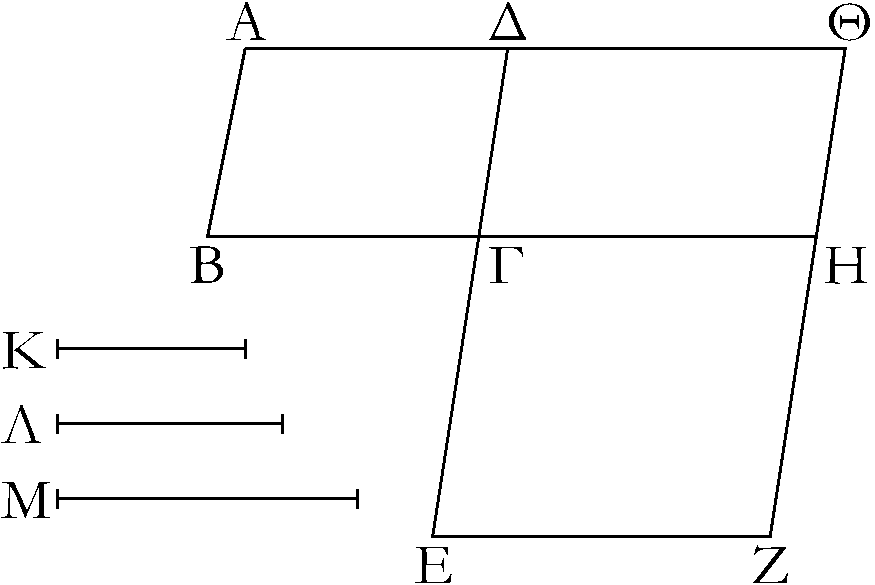
\includegraphics{Book06/fig23g.pdf}}

\gr{Κείσθω γὰρ <ώστε ἐπ> εὐθείαξ ε>ῖναι τὴν ΒΓ τῆ| ΓΗ; ἐπ> εὐθείαξ
>άρα ἐστὶ καὶ ἡ ΔΓ τῆ| ΓΕ. καὶ συμπεπληρώσθω τὸ ΔΗ
παραλληλόγραμμον, καὶ ἐκκείσθω τιξ εὐθεῖα
ἡ Κ, καὶ γεγονέτω ὡξ μὲν ἡ ΒΓ πρὸξ τὴν ΓΗ, ο<ύτωξ
ἡ Κ πρὸξ τὴν Λ, ὡξ δὲ ἡ ΔΓ πρὸξ τὴν ΓΕ, ο<ύτωξ ἡ Λ
πρὸξ τὴν Μ.}

\gr{Οἱ >άρα λόγοι τῆξ τε Κ πρὸξ τὴν Λ καὶ τῆξ Λ πρὸξ τὴν Μ οἱ
α\kern -.7pt  ὐτοί εἰσι τοῖξ λόγοιξ τῶν πλευρῶν, τῆξ τε ΒΓ πρὸξ τὴν
ΓΗ καὶ τῆξ ΔΓ πρὸξ τὴν ΓΕ. ἀλλ> ὁ τῆξ Κ πρὸξ Μ λόγοξ
σύγκειται >έκ τε τοῦ τῆξ Κ πρὸξ Λ λόγου καὶ τοῦ
τῆξ Λ πρὸξ Μ; <ώστε καὶ ἡ Κ πρὸξ τὴν Μ λόγον >έθει τὸν
συγκείμενον ἐκ τῶν πλευρῶν. καὶ ἐπεί ἐστιν ὡξ ἡ ΒΓ πρὸξ
τὴν ΓΗ, ο<ύτωξ τὸ ΑΓ παραλληλόγραμμον πρὸξ τὸ ΓΘ,
ἀλλ> ὡξ ἡ ΒΓ πρὸξ τὴν ΓΗ, ο<ύτωξ ἡ Κ πρὸξ τὴν Λ, καὶ
ὡξ >άρα ἡ Κ πρὸξ τὴν Λ, ο<ύτωξ τὸ ΑΓ πρὸξ τὸ ΓΘ. πάλιν,
ἐπεί ἐστιν ὡξ ἡ ΔΓ πρὸξ τὴν ΓΕ, ο<ύτωξ τὸ ΓΘ
παραλληλόγραμμον πρὸξ τὸ ΓΖ, ἀλλ> ὡξ ἡ ΔΓ πρὸξ τὴν ΓΕ,
ο<ύτωξ ἡ Λ πρὸξ τὴν Μ, καὶ ὡξ >άρα ἡ Λ πρὸξ τὴν Μ, ο<ύτωξ
τὸ ΓΘ παραλληλόγραμμον πρὸξ τὸ ΓΖ παραλληλόγραμμον. ἐπεὶ
ο>ῦν ἐδείθθη, ὡξ μὲν ἡ Κ πρὸξ τὴν Λ, ο<ύτωξ τὸ ΑΓ
παραλληλόγραμμον πρὸξ τὸ ΓΘ παραλληλόγραμμον, ὡξ
δὲ ἡ Λ πρὸξ τὴν Μ, ο<ύτωξ τὸ ΓΘ παραλληλόγραμμον πρὸξ
τὸ ΓΖ παραλληλόγραμμον, δι> >ίσου >άρα ἐστὶν ὡξ ἡ Κ πρὸξ
τὴν Μ, ο<ύτωξ τὸ ΑΓ πρὸξ τὸ ΓΖ παραλληλόγραμμον. ἡ δὲ Κ
πρὸξ τὴν Μ λόγον >έθει τὸν συγκείμενον ἐκ τῶν πλευρῶν;
καὶ τὸ ΑΓ >άρα πρὸξ τὸ ΓΖ λόγον >έθει τὸν συγκείμενον
ἐκ τῶν πλευρῶν.}

\gr{Τὰ >άρα ἰσογώνια παραλληλόγραμμα πρὸξ >άλληλα λόγον >έθει τὸν
συγκείμενον ἐκ τῶν πλευρῶν; <όπερ >έδει δεῖχαι.}}

\ParallelRText{
\begin{center}
{\large Proposition 23}
\end{center}

Equiangular parallelograms have to one another the ratio compounded$^\dag$ out of  (the ratios of) their sides.

Let $AC$ and $CF$ be equiangular parallelograms having angle $BCD$ equal to
$ECG$. I say that parallelogram $AC$ has to parallelogram $CF$ the ratio compounded out of (the ratios of) their sides.

% Removed epsf size command
\centerline{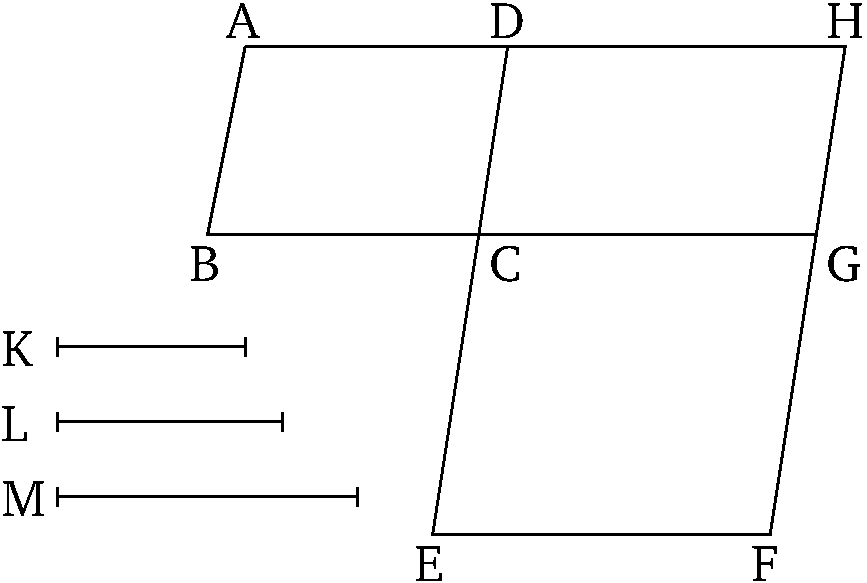
\includegraphics{Book06/fig23e.pdf}}

For let $BC$ be laid down so as to be straight-on to $CG$. Thus, $DC$ is also straight-on
to $CE$ [Prop.~1.14]. And let the parallelogram $DG$ be completed. And let
some straight-line $K$ be laid down. And let it be contrived that as $BC$ (is) to $CG$, so $K$ (is) to $L$, and as $DC$ (is) to $CE$,
so $L$ (is) to $M$ [Prop.~6.12].

Thus, the ratios of $K$ to $L$ and of $L$ to $M$ are the same as the ratios
of the sides, (namely), $BC$ to $CG$ and $DC$ to $CE$ (respectively). 
But, the ratio of $K$ to $M$ is compounded out of the ratio of $K$ to $L$
and (the ratio) of $L$ to $M$. Hence, $K$ also has to $M$ the ratio compounded out of
(the ratios of)  the sides
(of the parallelograms).
And since as $BC$ is to $CG$, so parallelogram $AC$ (is) to $CH$ [Prop.~6.1], but as $BC$ (is) to $CG$, so 
$K$ (is) to $L$, thus, also, as $K$ (is) to $L$, so (parallelogram) $AC$ (is) to $CH$.
Again, since as $DC$ (is) to $CE$, so parallelogram $CH$ (is) to $CF$
[Prop.~6.1], but 
as $DC$ (is) to $CE$, so $L$ (is) to $M$, thus, also, as $L$ (is) to $M$, so parallelogram
$CH$ (is) to parallelogram $CF$. Therefore, since it was shown that as $K$
(is) to $L$, so parallelogram $AC$ (is) to parallelogram $CH$, and as $L$ (is)
to $M$, so parallelogram $CH$ (is) to parallelogram $CF$, thus, via equality, 
as $K$ is to $M$, so (parallelogram) $AC$ (is) to parallelogram $CF$ [Prop.~5.22]. And $K$ has to $M$ the ratio compounded
out of (the ratios of) the  sides (of the parallelograms). Thus, (parallelogram) $AC$
also has to (parallelogram) $CF$ the ratio compounded out of (the ratio of) their sides.

Thus, equiangular parallelograms have to one another the ratio compounded out of (the ratio  of)  their sides. (Which is) the very thing it was required to show.}
\end{Parallel}
{\footnotesize\noindent$^\dag$ In modern terminology, if two
ratios are ``compounded'' then they are multiplied together.}

%%%%%%
% Prop 6.24
%%%%%%
\pdfbookmark[1]{Proposition 6.24}{pdf6.24}
\begin{Parallel}{}{} 
\ParallelLText{
\begin{center}
{\large \ggn{24}.}
\end{center}\vspace*{-7pt}

\gr{Παντὸξ παραλληλογράμμου τὰ περὶ τὴν διάμετρον παραλληλόγραμμα <όμοιά ἐστι τῶ| τε <όλῳ καὶ ἀλλήλοιξ.}

\gr{>'Εστω παραλληλόγραμμον τὸ ΑΒΓΔ, διάμετροξ δὲ α\kern -.7pt  ὐτοῦ ἡ ΑΓ,
περὶ δὲ τὴν ΑΓ παραλληλόγραμμα >έστω τὰ ΕΗ, ΘΚ; λέγω, <ότι
ἑκάτερον τῶν ΕΗ, ΘΚ παραλληλογράμμων <όμοιόν ἐστι
<όλῳ τῶ| ΑΒΓΔ καὶ ἀλλήλοιξ.}

% Removed epsf size command
\centerline{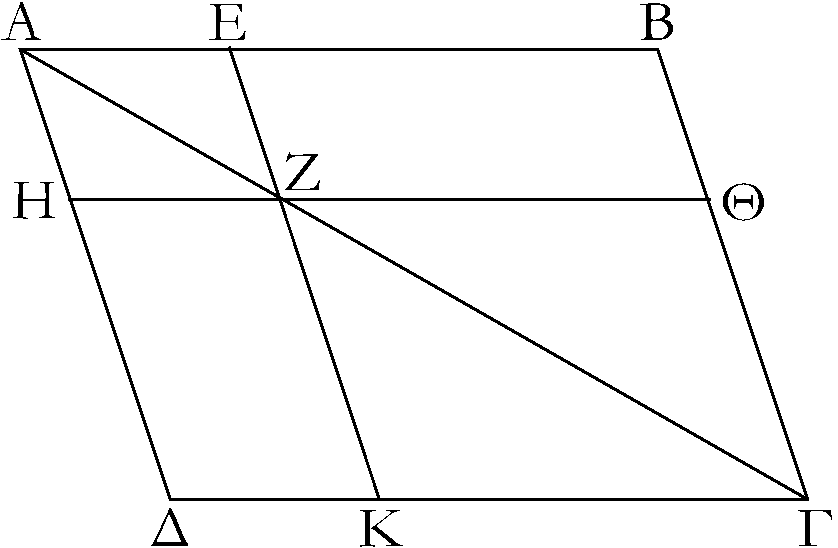
\includegraphics{Book06/fig24g.pdf}}

\gr{Ἐπεὶ γὰρ τριγώνου τοῦ ΑΒΓ παρὰ μίαν τῶν πλευρῶν τὴν
ΒΓ >ῆκται ἡ ΕΖ, ἀνάλογόν ἐστιν ὡξ ἡ ΒΕ πρὸξ τὴν ΕΑ, ο<ύτωξ
ἡ ΓΖ πρὸξ τὴν ΖΑ. πάλιν, ἐπεὶ τριγώνου τοῦ ΑΓΔ παρὰ μίαν
τὴν ΓΔ >ῆκται ἡ ΖΗ, ἀνάλογόν ἐστιν ὡξ ἡ ΓΖ πρὸξ τὴν
ΖΑ, ο<ύτωξ ἡ ΔΗ πρὸξ τὴν ΗΑ. ἀλλ> ὡξ ἡ ΓΖ πρὸξ τὴν ΖΑ,
ο<ύτωξ ἐδείθθη καὶ ἡ ΒΕ πρὸξ τὴν ΕΑ; καὶ ὡξ >άρα ἡ ΒΕ
πρὸξ τὴν ΕΑ, ο<ύτωξ ἡ 
ΔΗ πρὸξ τὴν ΗΑ, καὶ συνθέντι
>άρα ὡξ ἡ ΒΑ πρὸξ  ΑΕ, ο<ύτωξ ἡ ΔΑ πρὸξ ΑΗ, καὶ ἐναλλὰχ ὡξ
ἡ ΒΑ πρὸξ τὴν
ΑΔ, ο<ύτωξ ἡ ΕΑ πρὸξ
τὴν ΑΗ. τῶν >άρα ΑΒΓΔ, ΕΗ παραλληλογράμμων 
ἀνάλογόν εἰσιν αἱ πλευραὶ αἱ περὶ τὴν κοινὴν γωνίαν
τὴν ὑπὸ ΒΑΔ. καὶ ἐπεὶ παράλληλόξ ἐστιν ἡ ΗΖ τῆ|  ΔΓ, >ίση
ἐστὶν ἡ μὲν ὑπὸ ΑΖΗ γωνία τῆ| ὑπὸ ΔΓΑ; καὶ κοινὴ
τῶν δύο τριγώνων τῶν ΑΔΓ, ΑΗΖ ἡ ὑπὸ ΔΑΓ γωνία;
ἰσογώνιον >άρα ἐστὶ τὸ ΑΔΓ τρίγωνον τῶ| ΑΗΖ τριγώνῳ. διὰ
τὰ α\kern -.7pt  ὐτὰ δὴ καὶ τὸ ΑΓΒ τρίγωνον ἰσογώνιόν ἐστι τῶ| ΑΖΕ τριγώνῳ,
καὶ <όλον τὸ ΑΒΓΔ παραλληλόγραμμον τῶ| ΕΗ παραλληλογράμμῳ
ἰσογώνιόν  ἐστιν. ἀνάλογον >άρα ἐστὶν ὡξ  ἡ ΑΔ πρὸξ τὴν
ΔΓ, ο<ύτωξ ἡ ΑΗ πρὸξ τὴν ΗΖ, ὡξ δὲ ἡ ΔΓ πρὸξ τὴν ΓΑ,
ο<ύτωξ ἡ ΗΖ πρὸξ τὴν ΖΑ, ὡξ δὲ ἡ ΑΓ πρὸξ τὴν ΓΒ, ο<ύτωξ
ἡ ΑΖ πρὸξ τὴν ΖΕ, καὶ >έτι ὡξ ἡ ΓΒ πρὸξ τὴν ΒΑ, ο<ύτωξ
ἡ ΖΕ πρὸξ τὴν ΕΑ. καὶ ἐπεὶ ἐδείθθη ὡξ μὲν ἡ ΔΓ πρὸξ τὴν
ΓΑ, ο<ύτωξ ἡ ΗΖ πρὸξ τὴν ΖΑ, ὡξ δὲ ἡ ΑΓ πρὸξ τὴν
ΓΒ, ο<ύτωξ ἡ ΑΖ πρὸξ τὴν ΖΕ, δι> >ίσου >άρα ἐστὶν ὡξ ἡ
ΔΓ πρὸξ τὴν ΓΒ, ο<ύτωξ ἡ ΗΖ πρὸξ τὴν ΖΕ. τῶν >άρα ΑΒΓΔ,
ΕΗ παραλληλογράμμων ἀνάλογόν εἰσιν αἱ πλευραὶ αἱ περὶ τὰξ
>ίσαξ γωνίαξ; <όμοιον >άρα ἐστὶ τὸ ΑΒΓΔ παραλληλογράμμον
 τῶ| ΕΗ παραλληλογράμμῳ.
διὰ τὰ α\kern -.7pt  ὐτὰ δὴ τὸ ΑΒΓΔ παραλληλόγραμμον καὶ τῶ| ΚΘ παραλληλογράμμῳ <όμοιόν ἐστιν; ἑκάτερον >άρα τῶν ΕΗ, ΘΚ
παραλληλογράμμων τῶ| ΑΒΓΔ [παραλληλογράμμῳ] <όμοιόν
ἐστιν. τὰ δὲ τῶ| α\kern -.5pt  ὐτῶ| εὐθυγράμμῳ <όμοια καὶ ἀλλήλοιξ
ἐστὶν <όμοια; καὶ τὸ ΕΗ >άρα παραλληλόγραμμον τῶ| ΘΚ
παραλληλογράμμῳ <όμοιόν ἐστιν.}

\gr{Παντὸξ >άρα παραλληλογράμμου τὰ περὶ τὴν διάμετ\-ρον παραλληλόγραμμα <όμοιά ἐστι τῶ| τε <όλῳ καὶ ἀλλήλοιξ; <όπερ >έδει δεῖχαι.}}

\ParallelRText{
\begin{center}
{\large Proposition 24}
\end{center}

In any parallelogram, the parallelograms
about the diagonal are similar to the whole, and to one another.

Let $ABCD$ be a parallelogram, and $AC$ its diagonal. And let
$EG$ and $HK$ be parallelograms about $AC$. I say that the
parallelograms $EG$ and $HK$ are each similar to the whole (parallelogram) $ABCD$, and
to one another.

% Removed epsf size command
\centerline{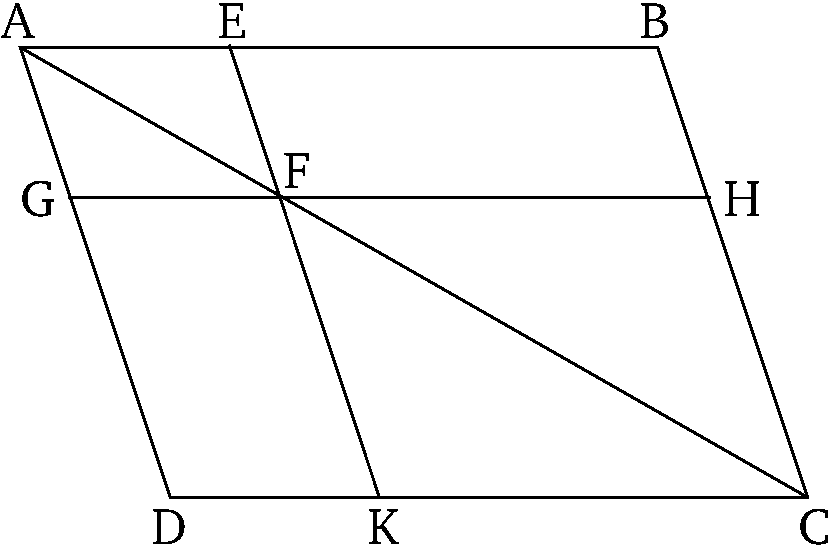
\includegraphics{Book06/fig24e.pdf}}

For since $EF$ has been drawn parallel to one of the sides $BC$ of triangle
$ABC$, proportionally, as $BE$ is to $EA$, so $CF$ (is) to $FA$ [Prop.~6.2]. Again, since $FG$ has been drawn
parallel to one (of the sides) $CD$ of triangle $ACD$, proportionally, 
as $CF$ is to $FA$, so $DG$ (is) to $GA$ [Prop.~6.2].
But, as $CF$ (is) to $FA$, so it was also shown (is) $BE$ to $EA$. And thus as
$BE$ (is) to $EA$, so $DG$ (is) to $GA$. And, thus, compounding, as $BA$ (is) to
$AE$, so $DA$ (is) to $AG$ [Prop.~5.18].
And, alternately, as $BA$ (is) to $AD$, so $EA$ (is) to $AG$ [Prop.~5.16]. Thus, in parallelograms
$ABCD$ and $EG$, the sides about the common angle $BAD$ are proportional.
And since $GF$ is parallel to $DC$, angle $AFG$ is equal to $DCA$  [Prop.~1.29]. And angle $DAC$ (is) common to the two triangles $ADC$ and
$AGF$. Thus, triangle $ADC$ is equiangular to triangle $AGF$  [Prop.~1.32]. So, for the same (reasons), triangle $ACB$ is equiangular to triangle $AFE$,
and the whole parallelogram $ABCD$ is equiangular to parallelogram $EG$. Thus,
proportionally, as $AD$ (is) to $DC$, so $AG$ (is) to $GF$, and as $DC$ (is) to 
$CA$, so $GF$ (is) to $FA$, and as $AC$ (is) to $CB$, so $AF$ (is) to $FE$, and, further, 
as $CB$ (is) to $BA$, so $FE$ (is) to $EA$ [Prop.~6.4].
And since it was shown that as $DC$  is to $CA$, so $GF$ (is) to $FA$, and
as $AC$ (is) to $CB$, so $AF$ (is) to $FE$, thus, via equality, as $DC$ is to $CB$,
so $GF$ (is) to $FE$ [Prop.~5.22]. 
Thus, in parallelograms $ABCD$ and $EG$, the sides about the equal angles are
proportional. Thus, parallelogram $ABCD$ is similar to parallelogram $EG$ [Def.~6.1]. So, for the same (reasons), 
parallelogram $ABCD$ is also similar to parallelogram $KH$. Thus, parallelograms $EG$ and $HK$ are each similar to [parallelogram] $ABCD$.
And (rectilinear figures) similar to the same rectilinear figure are also
similar to one another [Prop.~6.21].
Thus, parallelogram $EG$ is also similar to parallelogram $HK$.

Thus, in any parallelogram, the parallelograms
about the diagonal are similar to the whole, and to one another.
(Which is) the very thing it was required to show.}
\end{Parallel}

%%%%%%
% Prop 6.25
%%%%%%
\pdfbookmark[1]{Proposition 6.25}{pdf6.25}
\begin{Parallel}{}{} 
\ParallelLText{
\begin{center}
{\large \ggn{25}.}
\end{center}\vspace*{-7pt}

\gr{Τῶ| δοθέντι εὐθυγράμμῳ <όμοιον καὶ >άλλῳ τῶ| δοθέντι
>ίσον τὸ α\kern -.7pt  ὐτὸ συστήσασθαι.}\\

% Removed epsf size command
\centerline{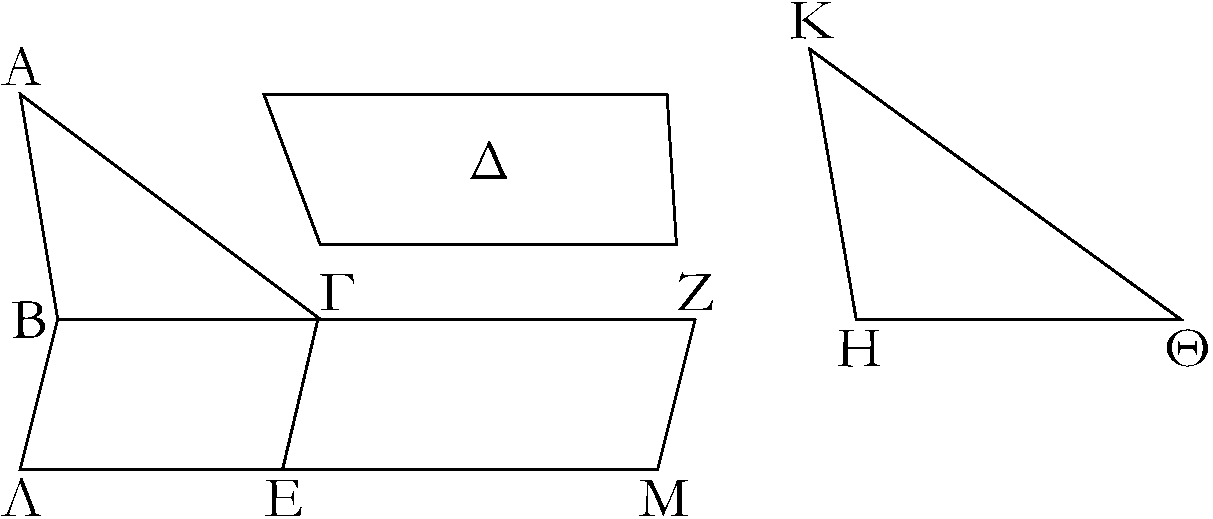
\includegraphics{Book06/fig25g.pdf}}

\gr{>'Εστω τὸ μὲν δοθὲν εὐθύγραμμον, <ῶ| δεῖ <όμοιον
συστήσασθ\-αι, τὸ ΑΒΓ, <ῶ| δὲ δεῖ >ίσον, τὸ Δ; δεῖ δὴ
τῶ| μὲν ΑΒΓ <όμοιον, τῶ| δὲ Δ >ίσον τὸ α\kern -.7pt  ὐτὸ
συστήσασθαι.}

\gr{Παραβεβλήσθω γὰρ παρὰ μὲν τὴν ΒΓ τῶ| ΑΒΓ τριγώνῳ >ίσον
παραλληλόγραμμον τὸ ΒΕ, παρὰ δὲ τὴν ΓΕ τῶ| Δ >ίσον παραλληλόγραμμον τὸ ΓΜ ἐν γωνίᾳ τῆ| ὑπὸ ΖΓΕ, <ή ἐστιν
>ίση τῆ| ὑπὸ ΓΒΛ. ἐπ> εὐθείαξ >άρα ἐστὶν ἡ μὲν ΒΓ
τῆ| ΓΖ, ἡ δὲ ΛΕ τῆ| ΕΜ. καὶ
εἰλήφθω τῶν ΒΓ, ΓΖ
μέση ἀνάλογον ἡ ΗΘ, καὶ ἀναγεγράφθω ἀπὸ τῆξ ΗΘ τῶ|
ΑΒΓ <όμοιόν τε καὶ ὁμοίωξ κείμενον τὸ ΚΗΘ.}

\gr{Καὶ ἐπεί ἐστιν ὡξ ἡ ΒΓ πρὸξ τὴν ΗΘ, ο<ύτωξ
ἡ ΗΘ πρὸξ τὴν ΓΖ, ἒαν δὲ τρεῖξ εὐθεῖαι ἀνάλογον
>ῶσιν, >έστιν ὡξ ἡ πρώτη πρὸξ τὴν τρίτην, ο<ύτωξ τὸ
ἀπὸ τῆξ πρώτηξ ε>ῖδοξ
πρὸξ τὸ ἀπὸ τῆξ δευτέραξ
τὸ <όμοιον καὶ ὁμοίωξ ἀναγραφόμενον, >έστιν >άρα ὡξ
ἡ ΒΓ πρὸξ τὴν ΓΖ, ο<ύτωξ τὸ ΑΒΓ τρίγωνον πρὸξ τὸ ΚΗΘ
τρίγωνον. ἀλλὰ καὶ ὡξ ἡ ΒΓ πρὸξ τὴν ΓΖ, ο<ύτωξ τὸ ΒΕ
παραλληλόγραμμον πρὸξ τὸ ΕΖ παραλληλόγραμμον. καὶ ὡξ >άρα
τὸ ΑΒΓ τρίγωνον πρὸξ τὸ ΚΗΘ τρίγωνον, ο<ύτωξ τὸ ΒΕ
παραλληλόγραμμον πρὸξ τὸ ΕΖ παραλληλόγραμμον; ἐναλλὰχ >άρα
ὡξ τὸ ΑΒΓ τρίγωνον πρὸξ τὸ ΒΕ παραλληλόγραμμον, ο<ύτωξ
τὸ ΚΗΘ τρίγωνον πρὸξ τὸ ΕΖ παραλληλόγραμμον. >ίσον δὲ τὸ ΑΒΓ
τρίγωνον τῶ| ΒΕ παραλληλογράμμῳ; >ίσον >άρα καὶ τὸ ΚΗΘ
τρίγωνον τῶ| ΕΖ παραλληλογράμμῳ. ἀλλὰ τὸ ΕΖ παραλληλόγραμμον
τῶ| Δ ἐστιν >ίσον; καὶ τὸ ΚΗΘ >άρα τῶ| Δ ἐστιν >ίσον. >έστι
δὲ τὸ ΚΗΘ καὶ τῶ| ΑΒΓ <όμοιον.}

\gr{Τῶ| >άρα δοθέντι εὐθυγράμμῳ  τῶ| ΑΒΓ <όμοιον καὶ >άλλῳ τῶ| δοθέντι τῶ| Δ
>ίσον τὸ α\kern -.7pt  ὐτὸ συνέσταται τὸ ΚΗΘ; <όπερ >έδει ποιῆσαι.}}

\ParallelRText{
\begin{center}
{\large Proposition 25}
\end{center}

To
 construct a single (rectilinear figure) similar to a given rectilinear figure, and equal to
a different given rectilinear figure.

% Removed epsf size command
\centerline{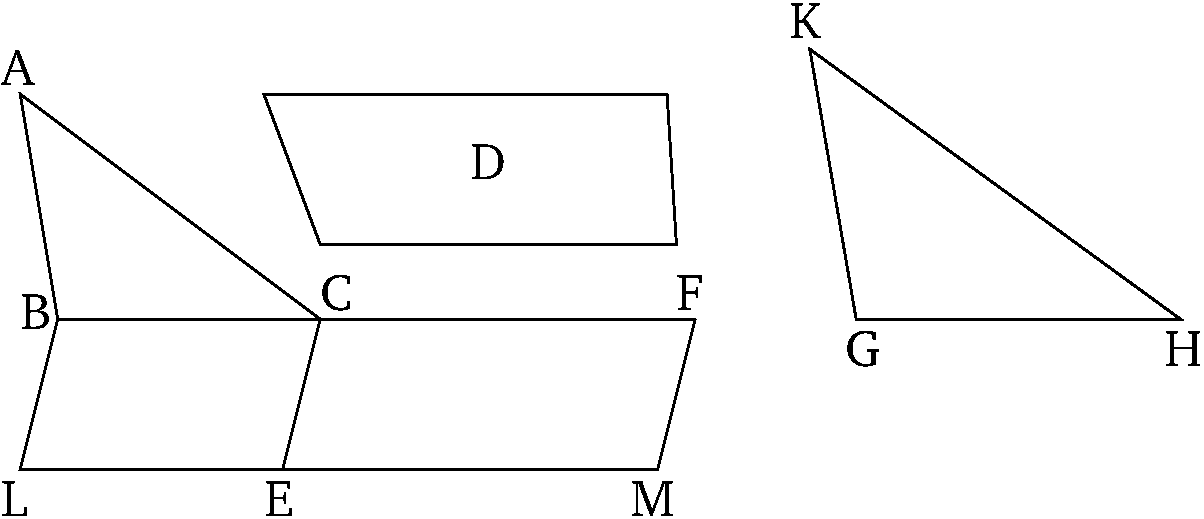
\includegraphics{Book06/fig25e.pdf}}

Let $ABC$ be the given rectilinear figure to which it is required to construct
a similar (rectilinear figure), and $D$ the (rectilinear figure) to which (the constructed figure) is required (to be) equal. So it is required to
construct a single (rectilinear figure) similar to $ABC$, and equal to $D$.

For  let the parallelogram $BE$, equal to triangle $ABC$, be applied to
(the straight-line) $BC$  [Prop.~1.44], and the parallelogram $CM$, equal to $D$, (be applied) to (the straight-line) $CE$,  in the angle $FCE$, which is equal to $CBL$  [Prop.~1.45]. Thus, $BC$ is
straight-on to $CF$, and $LE$ to $EM$ [Prop.~1.14]. And let the mean proportion $GH$ 
be taken of $BC$ and $CF$  [Prop.~6.13].
And let $KGH$, similar, and similarly laid out, to  $ABC$, be described
on $GH$ [Prop.~6.18].

And since as $BC$ is to $GH$, so $GH$ (is) to $CF$, and if three straight-lines are
proportional, (then) as the first is to the third, so the figure (described) on the first
(is) to the similar, and similarly described, (figure) on the second 
[Prop.~6.19~corr.],  thus as $BC$ is to
$CF$, so triangle $ABC$ (is) to triangle $KGH$. But, also, as $BC$ (is) to
$CF$, so parallelogram $BE$ (is) to parallelogram $EF$ [Prop.~6.1]. And, thus,  as triangle $ABC$ (is) to triangle $KGH$, so parallelogram $BE$ (is) to parallelogram $EF$. 
Thus, alternately, as triangle
$ABC$ (is) to parallelogram $BE$, so triangle $KGH$ (is) to
parallelogram $EF$ [Prop.~5.16]. 
And triangle $ABC$ (is) equal to parallelogram $BE$. Thus, triangle $KGH$
(is) also equal to parallelogram $EF$. But, parallelogram $EF$ is equal to $D$. 
Thus, $KGH$ is also equal to $D$. And $KGH$ is also similar to $ABC$.

Thus, a single (rectilinear figure) $KGH$ has been constructed (which is)
similar to the given rectilinear figure $ABC$, and equal to a different
given (rectilinear figure) $D$. (Which is) the very thing it was required to do.}
\end{Parallel}

%%%%%%
% Prop 6.26
%%%%%%
\pdfbookmark[1]{Proposition 6.26}{pdf6.26}
\begin{Parallel}{}{} 
\ParallelLText{
\begin{center}
{\large \ggn{26}.}
\end{center}\vspace*{-7pt}

\gr{Ἐὰν ἀπὸ παραλληλογράμμου παραλληλόγραμμον ἀφαιρεθῆ|
<όμοιόν τε τῶ| <όλῳ καὶ ὁμοίωξ κείμενον κοινὴν γωνίαν
>έθον α\kern -.7pt  ὐτῶ|, περὶ τὴν α\kern -.7pt  ὐτὴν διάμετρόν ἐστι τῶ| <όλῳ.}

\gr{Ἀπὸ γὰρ παραλληλογράμμου τοῦ ΑΒΓΔ παραλληλόγρα\-μμον
ἀφῃρήσθω τὸ ΑΖ <όμοιον τῶ| ΑΒΓΔ καὶ ὁμοίωξ κείμενον
κοινὴν γωνίαν >έθον α\kern -.7pt  ὐτῶ| τὴν ὑπὸ ΔΑΒ; λέγω, <ότι
περὶ τὴν α\kern -.7pt  ὐτὴν διάμετρόν ἐστι τὸ ΑΒΓΔ τῶ| ΑΖ.}\\

% Removed epsf size command
\centerline{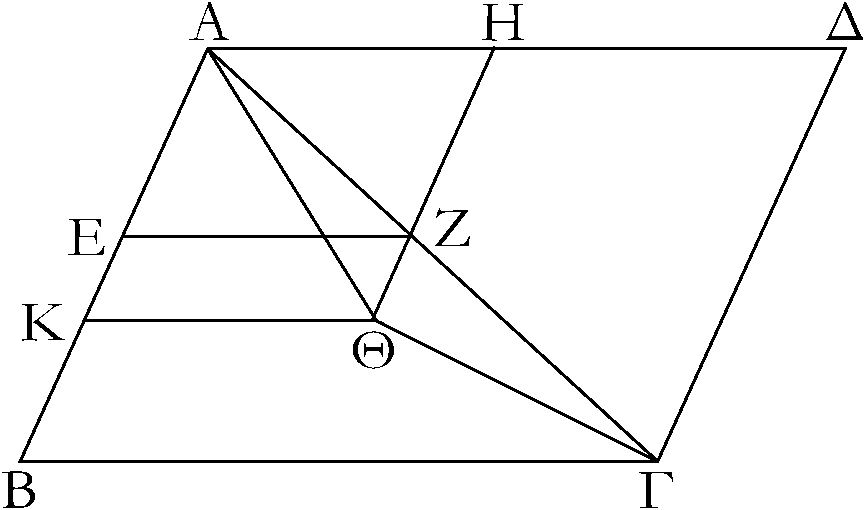
\includegraphics{Book06/fig26g.pdf}}

\gr{μ\kern -.7pt  ὴ γάρ, ἀλλ> εἰ δυνατόν, >έστω [α\kern -.7pt  ὐτῶν] διάμετροξ
ἡ ΑΘΓ, καὶ ἐκβληθεῖσα ἡ ΗΖ διήθθω ἐπὶ τὸ Θ, καὶ >ήθθω
διὰ τοῦ Θ ὁπορέρᾳ τῶν ΑΔ, ΒΓ παράλληλοξ ἡ ΘΚ.}

\gr{Ἐπεὶ ο>ῦν περὶ τὴν α\kern -.7pt  ὐτὴν διάμετρόν ἐστι τὸ ΑΒΓΔ τῶ| ΚΗ,
>έστιν >άρα ὡξ ἡ ΔΑ πρὸξ τὴν ΑΒ, ο<ύτωξ ἡ ΗΑ πρὸξ τὴν ΑΚ.
>έστι δὲ καὶ διὰ τὴν ὁμοιότητα τῶν ΑΒΓΔ, ΕΗ καὶ ὡξ ἡ ΔΑ
πρὸξ τὴν ΑΒ, ο<ύτωξ ἡ ΗΑ πρὸξ τὴν ΑΕ; καὶ ὡξ >άρα ἡ ΗΑ
πρὸξ τὴν ΑΚ, ο<ύτωξ ἡ ΗΑ πρὸξ  τὴν ΑΕ. ἡ ΗΑ >άρα πρὸξ 
ἑκατέραν τῶν ΑΚ, ΑΕ τὸν α\kern -.7pt  ὐτὸν >έθει λόγον. >ίση
>άρα ἐστὶν ἡ ΑΕ τῆ| ΑΚ ἡ ἐλάττων τῆ| μείζονι; <όπερ
ἐστὶν ἀδύνατον. οὐκ >άρα ο>ύκ ἐστι περὶ τὴν α\kern -.5pt  ὐτὴν
διάμετρον τὸ ΑΒΓΔ τῶ| ΑΖ; περὶ τὴν α\kern -.3pt  ὐτὴν >άρα ἐστὶ διάμετρον
τὸ ΑΒΓΔ παραλληλόγραμμον τῶ| ΑΖ παραλληλογράμμῳ.}

\gr{Ἐὰν >άρα ἀπὸ παραλληλογράμμου παραλληλόγραμ\-μον ἀφαιρεθῆ|
<όμοιόν τε τῶ| <όλῳ καὶ ὁμοίωξ κείμενον κοινὴν γωνίαν
>έθον α\kern -.7pt  ὐτῶ|, περὶ τὴν α\kern -.7pt  ὐτὴν διάμετρόν ἐστι τῶ| <όλῳ;
<όπερ >έδει δεῖχαι.}}

\ParallelRText{
\begin{center}
{\large Proposition 26}
\end{center}

If from a parallelogram a(nother) parallelogram
is subtracted (which is) similar, and similarly laid out, to the whole,
having a common angle with it, (then the subtracted parallelogram) is about the same diagonal
as the whole. 

For, from parallelogram $ABCD$, let (parallelogram) $AF$ be
subtracted (which is) similar, and similarly laid out,  to $ABCD$,
having  the common angle $DAB$ with it. I say that $ABCD$ is about
the same diagonal as $AF$.

% Removed epsf size command
\centerline{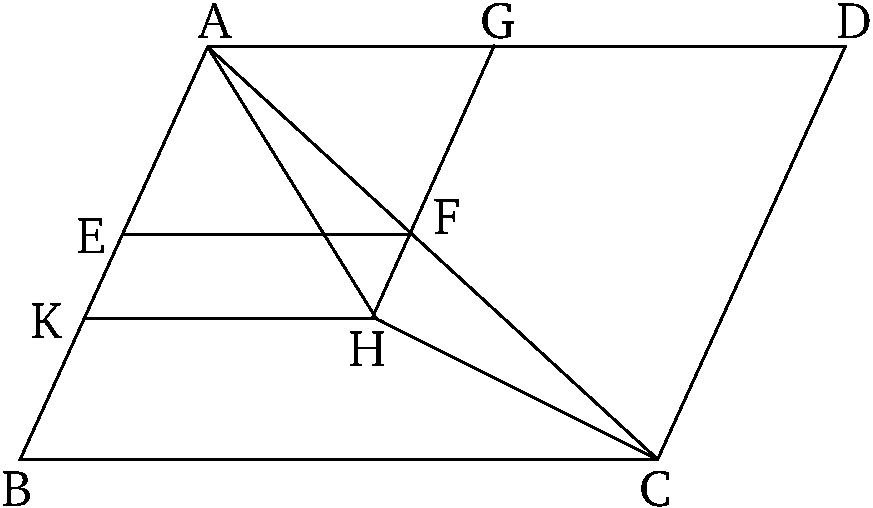
\includegraphics{Book06/fig26e.pdf}}

For (if) not, (then), if possible, let $AHC$ be [$ABCD$'s] diagonal. And producing
$GF$, let it be drawn through to (point) $H$. And let $HK$ 
be drawn through (point) $H$, parallel to either of $AD$ or $BC$  [Prop.~1.31].

Therefore, since $ABCD$ is about the same diagonal as $KG$, thus as
$DA$ is to $AB$, so $GA$ (is) to $AK$ [Prop.~6.24].
And, on account of the similarity of $ABCD$ and $EG$, also, as $DA$ (is)
to $AB$, so $GA$ (is) to $AE$. Thus, also, as $GA$ (is) to $AK$, so $GA$ (is)
to $AE$. Thus, $GA$ has the same ratio  to each of $AK$ and $AE$. Thus, 
$AE$ is equal to $AK$ [Prop.~5.9], the
lesser to the greater. The very thing is impossible. Thus, $ABCD$ is not not
about the same diagonal as $AF$. Thus, parallelogram $ABCD$ is
about the same diagonal as parallelogram $AF$.

Thus, if from a parallelogram a(nother) parallelogram
is subtracted (which is) similar, and similarly laid out, to the whole,
having a common angle with it, (then the subtracted parallelogram) is about the same diagonal
as the whole. (Which is) the very thing it was required to show.}
\end{Parallel}

%%%%%%
% Prop 6.27
%%%%%%
\pdfbookmark[1]{Proposition 6.27}{pdf6.27}
\begin{Parallel}{}{} 
\ParallelLText{
\begin{center}
{\large\ggn{27}.}
\end{center}\vspace*{-7pt}

\gr{Πάντων τῶν παρὰ τὴν α\kern -.7pt  ὐτὴν εὐθεῖαν παραβαλλομένων παραλληλογράμμων καὶ ἐλλειπόντων ε>ίδεσι παραλληλογράμ\-μοιξ
ὁμοίοιξ τε καὶ ὁμοίωξ κειμένοιξ τῶ| ἀπὸ τῆξ ἡμισείαξ
ἀναγραφομένῳ μέγιστόν ἐστι τὸ ἀπὸ τῆξ ἡμισείαξ
παραβαλλόμενον [παραλληλόγραμμον] <όμοιον >ὸν τῶ| ἐλλείμμαντι.}

\gr{>'Εστω εὐθεῖα ἡ ΑΒ καὶ τετμ\kern -.7pt  ήσθω δίθα κατὰ τὸ Γ, καὶ παραβεβλήσθω
παρὰ τὴν ΑΒ εὐθεῖαν τὸ ΑΔ παραλληλόγραμμον ἐλλεῖπον ε>ίδει
παραλληλογράμμῳ τῶ| ΔΒ ἀναγραφέντι ἀπὸ τῆξ ἡμισείαξ
τῆξ ΑΒ, τουτέστι τῆξ ΓΒ; λέγω, <ότι πάντων τῶν παρὰ τὴν ΑΒ
παραβαλλομένων παραλληλογράμμων καὶ ἐλλειπ\-όντων ε>ίδεσι
[παραλληλογράμμοιξ] ὁμοίοιξ τε καὶ ὁμοίωξ κειμένοιξ τῶ| ΔΒ
μέγιστόν ἐστι τὸ ΑΔ. παραβεβλήσθω γὰρ παρὰ τὴν ΑΒ εὐθεῖαν
τὸ ΑΖ παραλληλόγραμμον ἐλλεῖπον ε>ίδει παραλληλογράμμῳ τῶ|
ΖΒ ὁμοίῳ τε καὶ ὁμοίωξ κειμένῳ τῶ| ΔΒ; λέγω, <ότι μεῖζόν
ἐστι τὸ ΑΔ τοῦ ΑΖ.}

% Removed epsf size command
\centerline{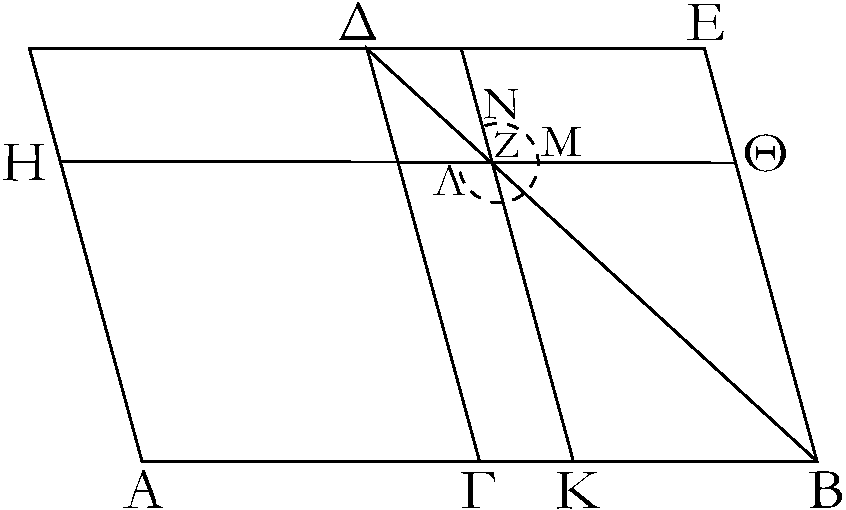
\includegraphics{Book06/fig27g.pdf}}

\gr{Ἐπεὶ γὰρ <όμοιόν ἐστι τὸ ΔΒ παραλληλόγραμμον τῶ| ΖΒ
παραλληλογράμμῳ, περὶ τὴν α\kern -.7pt  ὐτήν εἰσι διάμετρον. >ήθθω
α\kern -.7pt  ὐτῶν διάμετροξ ἡ ΔΒ, καὶ καταγεγράφθω τὸ σθῆμα.}

\gr{Ἐπεὶ ο>ῦν >ίσον ἐστὶ τὸ ΓΖ τῶ| ΖΕ, κοινὸν δὲ
τὸ ΖΒ, <όλον >άρα τὸ ΓΘ <όλῳ τῶ| ΚΕ ἐστιν >ίσον. ἀλλὰ τὸ
ΓΘ τῶ|  ΓΗ ἐστιν >ίσον, ἐπεὶ καὶ ἡ ΑΓ τῆ| ΓΒ. καὶ τὸ
ΗΓ >άρα τῶ| ΕΚ ἐστιν >ίσον. κοινὸν προσκείσθω τὸ ΓΖ; <όλον >άρα
τὸ ΑΖ τῶ| ΛΜΝ γνώμονί ἐστιν >ίσον; <ώστε τὸ ΔΒ παραλληλόγραμμον,
τουτέστι τὸ ΑΔ, τοῦ ΑΖ παραλληλογράμμου μεῖζόν ἐστιν.}

\gr{Πάντων >άρα τῶν παρὰ τὴν α\kern -.7pt  ὐτὴν εὐθεῖαν παραβαλλομένων
παραλληλογράμμων καὶ ἐλλειπόντων ε>ίδεσι παραλληλογράμμοιξ
ὁμοίοιξ τε καὶ ὁμοίωξ κειμένοιξ
τῶ| ἀπὸ τῆξ ἡμισείαξ ἀναγραφομένῳ μέγιστόν ἐστι τὸ
ἀπὸ τῆξ ἡμισείαξ παραβληθέν; <όπερ >έδει δεῖχαι.}}

\ParallelRText{
\begin{center}
{\large Proposition 27}
\end{center}

Of all the parallelograms applied to the
same straight-line, and falling short by parallelogrammic figures
similar, and similarly laid out, to the (parallelogram)
described on half (the straight-line), the greatest is the [parallelogram]
applied to half (the straight-line) which (is) similar to (that parallelogram)
by which it falls short.

Let $AB$ be a straight-line, and let it be cut in half at
(point) $C$ [Prop.~1.10]. And let the parallelogram $AD$ be applied to the straight-line
$AB$, 
falling short by the parallelogramic figure $DB$ (which is) applied to
half of $AB$---that is to say, $CB$. I say that of all  the parallelograms applied to $AB$, and
falling short by  [parallelogramic] figures similar, and similarly
laid out, to $DB$, the greatest is $AD$. For let the parallelogram
$AF$ be applied to the straight-line $AB$, falling short by
the parallelogramic figure $FB$ (which is) similar, and similarly laid out,
to $DB$. I say that $AD$ is greater than $AF$.

% Removed epsf size command
\centerline{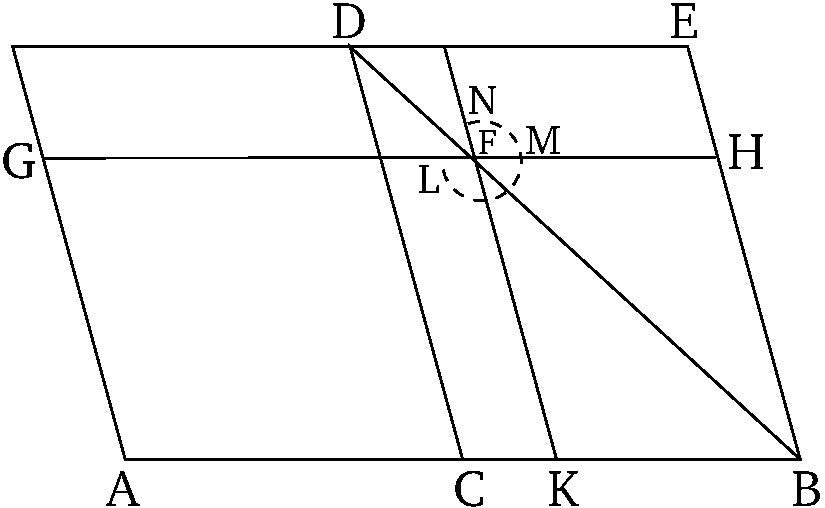
\includegraphics{Book06/fig27e.pdf}}

For since parallelogram $DB$ is similar to parallelogram $FB$, they are
about the same diagonal [Prop.~6.26].
Let their (common) diagonal $DB$ be drawn, and let the (rest of the)  figure be
described.

Therefore, since (complement) $CF$ is equal to (complement) $FE$  [Prop.~1.43],
and (parallelogram) $FB$ is common, the whole (parallelogram) $CH$ is thus
equal to the whole (parallelogram) $KE$. But, (parallelogram)
$CH$ is equal to $CG$, since $AC$ (is) also (equal) to $CB$ [Prop.~6.1]. Thus, (parallelogram) $GC$ is also equal to $EK$. 
Let (parallelogram) $CF$ be added to both. Thus, the whole (parallelogram) $AF$
is equal to the gnomon $LMN$. Hence, parallelogram $DB$---that is
to say, $AD$---is greater than parallelogram $AF$.

Thus, for all parallelograms applied to the
same straight-line, and falling short by a parallelogramic figure
similar, and similarly laid out, to the (parallelogram)
described on half (the straight-line), the greatest is the [parallelogram]
applied to half (the straight-line). (Which is) the very thing it was required
to show.}
\end{Parallel}

%%%%%%
% Prop 6.28
%%%%%%
\pdfbookmark[1]{Proposition 6.28}{pdf6.28}
\begin{Parallel}{}{} 
\ParallelLText{
\begin{center}
{\large \ggn{28}.}
\end{center}\vspace*{-7pt}

\gr{Παρὰ τὴν δοθεῖσαν εὐθεῖαν τῶ| δοθέντι εὐθυγράμμῳ >ίσον
παραλληλόγραμμον παραβαλεῖν ἐλλεῖπον ε>ίδει παραλληλογράμμῳ
ὁμοίῳ τῶ| δοθέντι; δεῖ δὲ τὸ διδόμενον εὐθύγραμμον
[<ῶ| δεῖ >ίσον παραβαλεῖν] μ\kern -.7pt  ὴ μεῖζον ε>ῖναι τοῦ ἀπὸ 
τῆξ ἡμισείαξ ἀναγραφομένου ὁμοίου τῶ|  ἐλλείμματι
[τοῦ τε ἀπὸ τῆξ ἡμισείαξ καὶ <ῶ| δεῖ <όμοιον
ἐλλείπειν].}

\gr{>'Εστω ἡ μὲν δοθεῖσα εὐθεῖα ἡ ΑΒ, τὸ δὲ δοθὲν εὐθύγραμμ\-ον,
<ῶ| δεῖ >ίσον παρὰ  τὴν ΑΒ παραβαλεῖν, τὸ Γ μ\kern -.7pt  ὴ μεῖζον
[>ὸν] τοῦ  ἀπὸ τῆξ ἡμισείαξ τῆξ ΑΒ ἀναγραφομένου ὁμοίου
τῶ| ἐλλείμματι, <ῶ| δὲ δεῖ <όμοιον
ἐλλείπειν, τὸ Δ; δεῖ δὴ παρὰ τὴν δοθεῖσαν εὐθεῖαν
τὴν ΑΒ τῶ| δοθέντι εὐθυγράμμῳ τῶ| Γ >ίσον
παραλληλόγραμμον παραβαλεῖν ἐλλεῖπον ε>ίδει παραλληλογράμμῳ
ὁμοίῳ >όντι τῶ| Δ.}

\gr{Τετμ\kern -.7pt  ήσθω ἡ ΑΒ δίθα κατὰ τὸ Ε σημεῖον, καὶ ἀναγεγράφθω
ἀπὸ τῆξ ΕΒ τῶ| Δ <όμοιον καὶ ὁμοίωξ κείμενον τὸ
ΕΒΖΗ, καὶ συμπεπληρώσθω τὸ ΑΗ παραλληλόγραμμον.}\\~\\~\\

% Removed epsf size command
\centerline{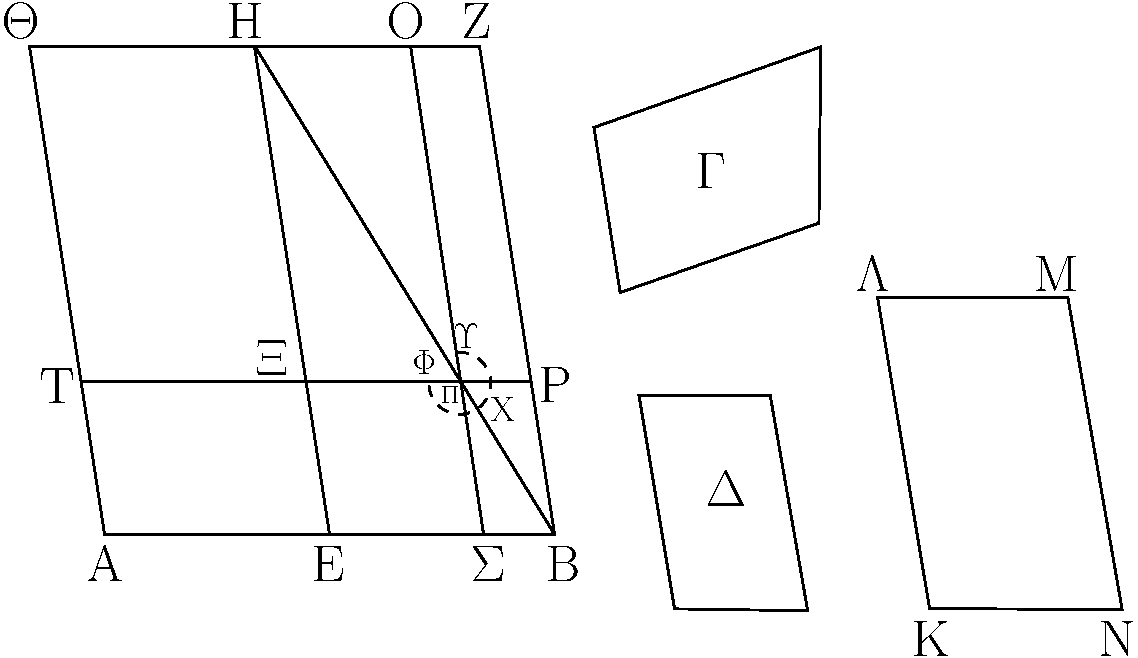
\includegraphics{Book06/fig28g.pdf}}

\gr{Εἰ μὲν ο>ῦν  >ίσον ἐστὶ τὸ ΑΗ τῶ| Γ, γεγονὸξ >ὰν
ε>ίη τὸ ἐπιταθθέν; παραβέβληται γὰρ παρὰ τὴν δοθεῖσαν
εὐθεῖαν τὴν ΑΒ τῶ| δοθέντι εὐθυγράμμῳ τῶ| Γ >ίσον
παραλληλόγραμμον τὸ ΑΗ ἐλλεῖπον ε>ίδει παραλληλογράμμῳ
τῶ| ΗΒ ὁμοίῳ  >όντι τῶ| Δ. εἰ δὲ ο>ύ, μεῖζόν >έστω τὸ
ΘΕ τοῦ Γ. >ίσον δὲ τὸ ΘΕ τῶ| ΗΒ; μεῖζον 
>άρα 
καὶ τὸ ΗΒ τοῦ Γ. <ῶ| δὴ μεῖζόν ἐστι τὸ ΗΒ τοῦ Γ, 
 τα\kern -.7pt  ύτῃ τῆ| ὑπεροθῆ| >ίσον, τῶ| δὲ Δ <όμοιον
καὶ ὁμοίωξ κείμενον τὸ α\kern -.7pt  ὐτὸ συνεστάτω τὸ ΚΛΜΝ. 
ἀλλὰ τὸ Δ τῶ| ΗΒ [ἐστιν] <όμοιον; καὶ τὸ ΚΜ >άρα τῶ| ΗΒ
ἐστιν <όμοιον. >έστω ο>ῦν ὁμόλογοξ ἡ μὲν ΚΛ τὴ| 
ΗΕ, ἡ δὲ ΛΜ τῆ| ΗΖ. καὶ ἐπεὶ >ίσον ἐστὶ τὸ ΗΒ τοῖξ 
Γ, ΚΜ, μεῖζον >άρα ἐστὶ τὸ ΗΒ τοῦ ΚΜ; μείζων >άρα
ἐστὶ καὶ ἡ μὲν ΗΕ τῆξ ΚΛ, ἡ δὲ ΗΖ τῆξ ΛΜ. κείσθω
τῆ| μὲν ΚΛ >ίση ἡ ΗΧ, τῆ| δὲ ΛΜ >ίση ἡ ΗΟ, καὶ
συμπεπληρώσθω τὸ ΧΗΟΠ παραλληλόγραμμον; >ίσον >άρα
καὶ <όμοιον ἐστι [τὸ ΗΠ] τῶ| ΚΜ [ἀλλὰ τὸ ΚΜ τῶ|
ΗΒ <όμοιόν ἐστιν]. καὶ τὸ ΗΠ >άρα τῶ| ΗΒ <όμοιόν ἐστιν;
περὶ τὴν α\kern -.5pt  ὐτὴν >άρα διάμετρόν ἐστι τὸ ΗΠ
τῶ| ΗΒ. >έστω α\kern -.3pt  ὐτῶν 
διάμετροξ ἡ ΗΠΒ, καὶ
καταγεγράφθω τὸ σθῆμα.}

\gr{Ἐπεὶ ο>ῦν >ίσον ἐστὶ τὸ ΒΗ τοῖξ Γ, ΚΜ, <ῶν
τὸ ΗΠ τῶ| ΚΜ ἐστιν >ίσον, λοιπὸξ >άρα ὁ ΥΘΦ γνόμων
λοιπῶ| τῶ| Γ >ίσοξ ἐστίν. καὶ ἐπεὶ >ίσον ἐστὶ τὸ 
ΟΡ τῶ| ΧΣ, κοινὸν προσκείσθω τὸ ΠΒ; <όλον >άρα
τὸ ΟΒ <όλῳ τῶ| ΧΒ >ίσον ἐστίν. ἀλλὰ τὸ ΧΒ τῶ|
ΤΕ ἐστιν >ίσον, ἐπεὶ καὶ πλευρὰ ἡ ΑΕ πλευρᾶ| τῆ|
ΕΒ ἐστιν >ίση; καὶ τὸ ΤΕ >άρα τῶ| ΟΒ ἐστιν >ίσον. κοινὸν
προσκείσθω τὸ ΧΣ; <όλον >άρα τὸ ΤΣ <όλῳ τῶ| ΦΘΥ
γνώμονί ἐστιν >ίσον. ἀλλ> ὁ ΦΘΥ γνώμων τῶ| Γ
ἐδείθθη >ίσοξ; καὶ τὸ ΤΣ >άρα τῶ| Γ ἐστιν >ίσον.}

\gr{Παρὰ τὴν δοθεῖσαν >άρα εὐθεῖαν τὴν ΑΒ τῶ| δοθέντι εὐθυγράμμῳ τῶ| Γ >ίσον
παραλληλόγραμμον παραβέβλ\-ηται τὸ ΣΤ  ἐλλεῖπον ε>ίδει παραλληλογράμμῳ
τῶ| ΠΒ ὁμοίῳ >όντι τῶ| Δ [ἐπειδήπερ τὸ ΠΒ τῶ| ΗΠ
<όμοιόν ἐστιν]; <όπερ  >έδει ποιῆσαι.}}

\ParallelRText{
\begin{center}
{\large Proposition 28}$^\dag$
\end{center}

To apply a parallelogram, equal to a given
rectilinear figure,  to a given
straight-line, (the applied parallelogram) falling short by a parallelogrammic figure similar to a given (parallelogram). It is necessary for the given rectilinear figure [to which it
is required to apply an equal (parallelogram)] not to be  greater than the (parallelogram)
described on half (of the straight-line) and similar to the deficit.

Let $AB$ be the given straight-line, and $C$ the given rectilinear figure to which
the (parallelogram) applied to $AB$ is required (to be) equal, [being] not
greater than the (parallelogram) described on half of $AB$ and
similar to the deficit, and $D$ the (parallelogram) to which the deficit is
required (to be) similar. So it is required to apply a parallelogram, equal to
the given rectilinear figure $C$, 
to the straight-line $AB$, falling short by a parallelogramic figure which
is similar to $D$.

Let $AB$ be cut in half at point $E$  [Prop.~1.10], and let (parallelogram) $EBFG$, (which is)
similar, and similarly laid out, to (parallelogram) $D$, be described on $EB$ 
[Prop.~6.18]. And let parallelogram
$AG$ be completed.

% Removed epsf size command
\centerline{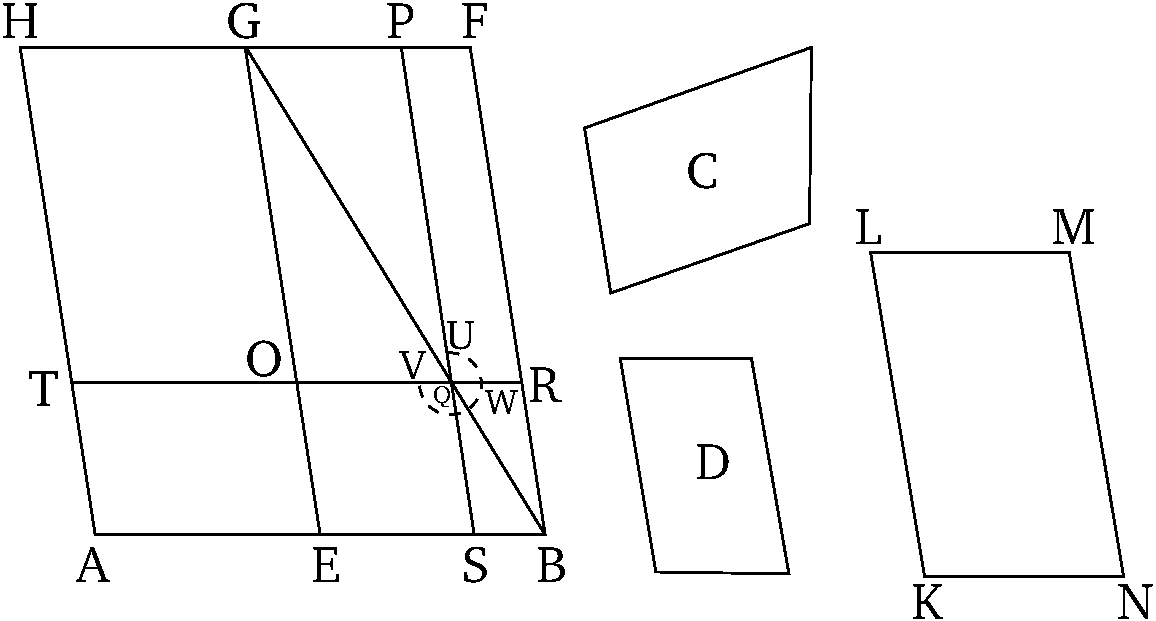
\includegraphics{Book06/fig28e.pdf}}

Therefore, if $AG$ is equal to $C$, (then) the thing prescribed has happened. For
a parallelogram  $AG$, equal to the given rectilinear figure $C$, has been
applied to the given straight-line $AB$, falling short by a parallelogramic
figure $GB$ which is similar to $D$. And if not,  let $HE$ be greater than $C$. 
And $HE$ (is) equal to $GB$ [Prop.~6.1]. 
Thus, $GB$ (is) also greater than $C$.
So, let (parallelogram) $KLMN$ be constructed (so as to be) both similar, and similarly laid out, to $D$,
and equal to the excess by which $GB$ is greater than $C$ [Prop.~6.25]. But, $GB$ [is] similar to
$D$. Thus, $KM$ is also similar to $GB$
[Prop.~6.21]. Therefore, let $KL$ correspond to
$GE$, and $LM$ to $GF$. And since (parallelogram) $GB$ is equal to
(figure) $C$ and (parallelogram) $KM$, $GB$ is thus greater than $KM$. Thus,
$GE$ is also greater than $KL$, and $GF$ than $LM$. Let $GO$ be made equal to
$KL$, and $GP$ to $LM$  [Prop.~1.3]. And let the parallelogram
$OGPQ$ be completed. Thus, [$GQ$] is equal and similar to
$KM$ [but, $KM$ is similar to $GB$]. Thus, $GQ$ is also similar to $GB$ [Prop.~6.21]. Thus, $GQ$ and $GB$ are about the
same diagonal [Prop.~6.26]. 
Let $GQB$ be their (common) diagonal, and let the (remainder of the) figure be described.

Therefore, since $BG$ is equal to $C$ and $KM$, of which $GQ$ is equal
to $KM$, the remaining gnomon $UWV$ is thus equal to the remainder $C$. 
And since (the complement) $PR$ is equal to (the complement) $OS$  [Prop.~1.43], let (parallelogram) $QB$ be added to both. Thus, the whole
(parallelogram) $PB$ is equal to the whole (parallelogram) $OB$. But,
$OB$ is equal to $TE$, since side $AE$ is equal to side $EB$ [Prop.~6.1]. Thus, $TE$ is also equal to $PB$. 
Let (parallelogram) $OS$ be added to both. Thus, the whole (parallelogram) $TS$ is equal to the gnomon $VWU$. But, gnomon $VWU$ was shown (to be)
equal to $C$.  Therefore, (parallelogram) $TS$ is also equal to (figure) $C$.

Thus, the parallelogram $ST$, equal to the given rectilinear figure
$C$, has been applied to the given straight-line $AB$, falling
short by the parallelogramic figure $QB$, which is similar to $D$ [inasmuch as
$QB$ is similar to $GQ$ [Prop.~6.24]\,]. 
(Which is) the very thing it was required to do.}
\end{Parallel}
{\footnotesize\noindent$^\dag$ This proposition is a geometric
solution of the quadratic equation $x^2 - \alpha\,x +\beta = 0$. Here,
$x$ is the ratio of a side of the deficit to the corresponding side of figure $D$, $\alpha$
is the ratio of the length of $AB$ to the length of that side of figure $D$ which corresponds to the side of the deficit running along $AB$, and $\beta$ is the
ratio of the areas of figures $C$ and $D$. The constraint corresponds to the
condition $\beta < \alpha^2/4$ for the equation to have real roots. Only the
smaller root of the equation is found. The larger root can be found by a
similar method.}

%%%%%%
% Prop 6.29
%%%%%%
\pdfbookmark[1]{Proposition 6.29}{pdf6.29}
\begin{Parallel}{}{} 
\ParallelLText{
\begin{center}
{\large \ggn{29}.}
\end{center}\vspace*{-7pt}

\gr{Παρὰ τὴν δοθεῖσαν εὐθεῖαν τῶ| δοθέντι εὐθυγράμμῳ >ίσον
παραλληλόγραμμον παραβαλεῖν ὑπερβάλλον ε>ίδει παραλληλογράμμῳ
ὁμοίῳ τῶ| δοθέντι.}\\

% Removed epsf size command
\centerline{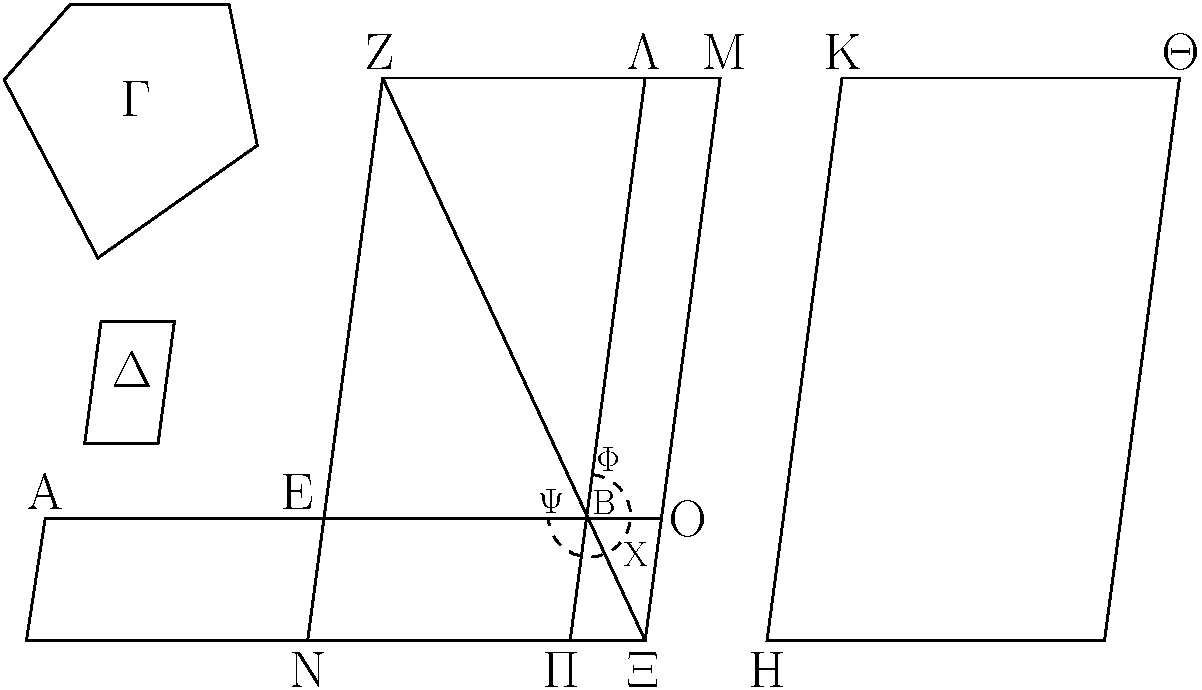
\includegraphics{Book06/fig29g.pdf}}

\gr{>'Εστω ἡ μὲν δοθεῖσα εὐθεῖα ἡ ΑΒ, τὸ δὲ δοθὲν εὐθύγραμμ\-ον,
<ῶ| δεῖ >ίσον παρὰ τὴν ΑΒ παραβαλεῖν, τὸ Γ, <ῶ| δὲ δεῖ
<όμοιον ὑπερβάλλειν, τὸ Δ; δεῖ δὴ παρὰ τὴν
ΑΒ εὐθεῖαν τῶ| Γ εὐθυγράμμῳ >ίσον παραλληλόγραμμον
παραβαλεῖν ὑπερβάλλον ε>ίδει παραλληλογράμμῳ ὁμοίῳ
τῶ| Δ.}

\gr{Τετμ\kern -.7pt  ήσθω ἡ ΑΒ δίθα κατὰ τὸ Ε, καὶ ἀναγεγράθω ἀπὸ τῆξ
ΕΒ τῶ| Δ <όμοιον καὶ ὁμοίωξ κείμενον
παραλληλόγραμμον τὸ ΒΖ, καὶ συναμφοτέροιξ μὲν τοῖξ ΒΖ, Γ
>ίσον, τῶ| δὲ Δ <όμοιον καὶ ὁμοίωξ
κείμενον τὸ α\kern -.7pt  ὐτὸ συνεστάτω τὸ ΗΘ. ὁμόλογοξ
δὲ >έστω ἡ μὲν ΚΘ τῆ| ΖΛ, ἡ δὲ ΚΗ τῆ| ΖΕ. καὶ ἐπεὶ μεῖζόν
ἐστι τὸ ΗΘ τοῦ ΖΒ, μείζων >άρα ἐστὶ καὶ ἡ μὲν ΚΘ τῆξ ΖΛ,
ἡ δὲ ΚΗ τῆ| ΖΕ. ἐκβεβλήσθωσαν
αἱ ΖΛ, ΖΕ, καὶ τῆ| μὲν ΚΘ >ίση >έστω ἡ
ΖΛΜ, τῆ| δὲ ΚΗ >ίση ἡ ΖΕΝ, καὶ συμπεπληρώσθω τὸ ΜΝ; τὸ
ΜΝ >άρα τῶ| ΗΘ >ίσον τέ ἐστι καὶ <όμοιον.
ἀλλὰ τὸ ΗΘ τῶ| ΕΛ ἐστιν <όμοιον; καὶ τὸ ΜΝ >άρα τῶ| ΕΛ <όμοιόν
ἐστιν; περὶ τὴν α\kern -.5pt  ὐτὴν >άρα διάμετρόν ἐστι τὸ ΕΛ τῶ| ΜΝ.
>ήθθω α\kern -.3pt  ὐτῶν διάμετροξ ἡ ΖΧ, καὶ καταγεγράφθω τὸ σθῆμα.}

\gr{Ἐπεὶ >ίσον ἐστὶ τὸ ΗΘ τοῖξ ΕΛ, Γ, ἀλλὰ τὸ ΗΘ τῶ| ΜΝ
>ίσον ἐστίν, καὶ τὸ ΜΝ >άρα τοῖξ ΕΛ, Γ
>ίσον ἐστίν. 
 κοινὸν ἀφῃρήσθω τὸ ΕΛ; λοιπὸξ >άρα ὁ ΨΘΦ γνώμων
 τῶ| Γ ἐστιν >ίσοξ. καὶ ἐπεὶ >ίση ἐστὶν ἡ ΑΕ τῆ| ΕΒ, >ίσον
ἐστὶ καὶ τὸ ΑΝ τῶ| ΝΒ, τουτέστι τῶ| ΛΟ. κοινὸν προσκείσθω
τὸ ΕΧ; <όλον >άρα τὸ  ΑΧ >ίσον ἐστὶ τῶ| ΦΘΨ γνώμονι.
ἀλλὰ ὁ ΦΘΨ γνώμων τῶ| Γ >ίσοξ ἐστίν; καὶ τὸ ΑΧ >άρα
τῶ| Γ >ίσον ἐστίν.}

\gr{Παρὰ τὴν δοθεῖσαν >άρα εὐθεῖαν τὴν ΑΒ τῶ|
δοθέντι εὐθυγράμμῳ τῶ| Γ >ίσον παραλληλόγραμμον
παραβέβλ\-ηται τὸ ΑΧ ὑπερβάλλον ε>ίδει παραλληλογράμμῳ τῶ| ΠΟ
ὁμοίῳ >όντι τῶ| Δ, ἐπεὶ καὶ τῶ| ΕΛ ἐστιν <όμοιον
τὸ ΟΠ;  <όπερ >έδει ποιῆσαι.}}

\ParallelRText{
\begin{center}
{\large Proposition 29}$^\dag$
\end{center}

To apply a parallelogram, equal to a given
rectilinear figure,  to a given
straight-line, (the applied parallelogram) overshooting by a parallelogramic figure similar to a given (parallelogram).

% Removed epsf size command
\centerline{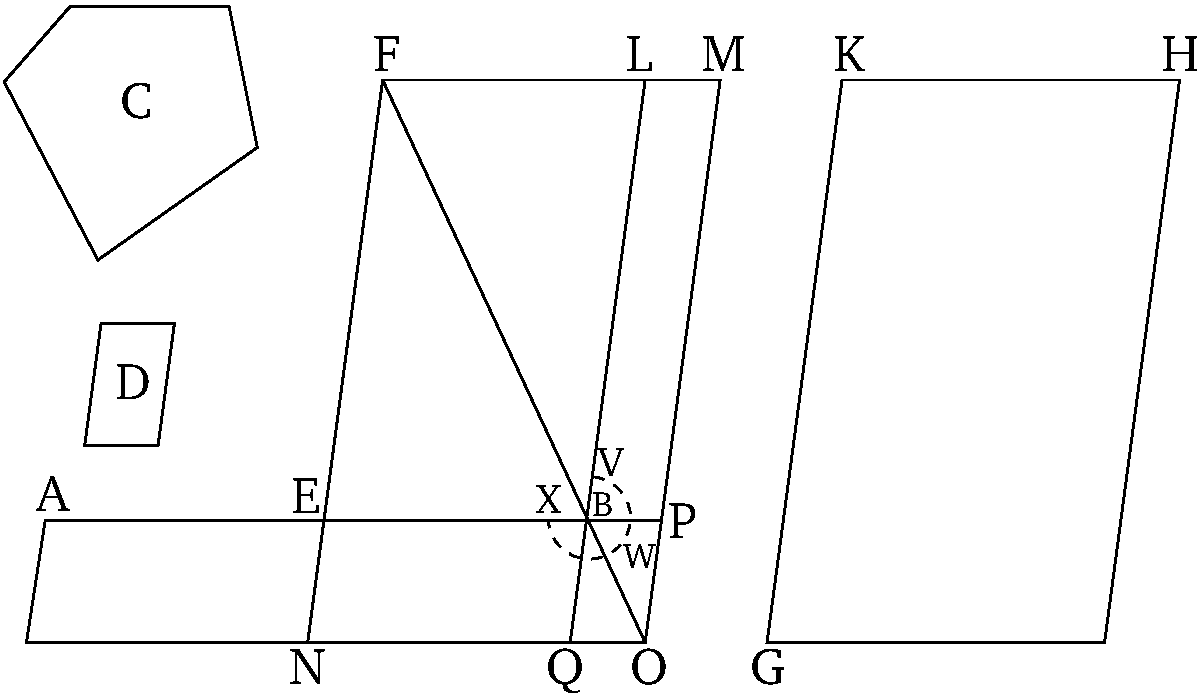
\includegraphics{Book06/fig29e.pdf}}

Let $AB$ be the given straight-line, and $C$ the given rectilinear figure to which the (parallelogram) applied to $AB$ is required (to be) equal, and $D$ the (parallelogram) to which the excess is required (to be) similar. So
it is required to apply a parallelogram, equal to the given rectilinear figure
$C$, to the given straight-line $AB$, overshooting by a parallelogrammic
figure  similar to $D$.

Let $AB$ be cut in half at (point) $E$  [Prop.~1.10], and
let the parallelogram $BF$, (which is) similar, and similarly laid out, to $D$,
be described on $EB$ [Prop.~6.18].
And let (parallelogram) $GH$ be constructed (so as to be) both similar, and similarly laid out, to $D$, and equal to the sum of $BF$ and $C$ [Prop.~6.25]. And let $KH$ correspond to
$FL$, and $KG$ to $FE$. And since (parallelogram) $GH$ is greater than 
(parallelogram) $FB$, $KH$ is thus
also greater than $FL$, and $KG$ than $FE$.  Let $FL$ and $FE$ be produced,
and let $FLM$ be (made) equal to $KH$, and $FEN$ to $KG$  [Prop.~1.3]. 
And let (parallelogram) $MN$ be completed. Thus, $MN$ is equal and
similar  to $GH$. But, $GH$ is similar to $EL$. Thus, $MN$  is also similar to
$EL$ [Prop.~6.21]. $EL$ is thus about the
same diagonal as $MN$ [Prop.~6.26]. 
Let their (common) diagonal $FO$ be drawn, and let the (remainder
of the) figure be described.

And since (parallelogram) $GH$ is equal to (parallelogram) $EL$ and (figure) $C$,
but $GH$ is equal to (parallelogram) $MN$, $MN$ is thus also equal to $EL$ and
$C$. Let $EL$ be subtracted from both. Thus, the remaining gnomon
$XWV$ is equal to (figure) $C$. And since $AE$ is equal to $EB$, (parallelogram)
$AN$ is also equal to (parallelogram) $NB$ [Prop.~6.1], that is to say, (parallelogram) $LP$  [Prop.~1.43]. Let
(parallelogram) $EO$ be added to both. Thus, the whole (parallelogram)
$AO$ is equal to the gnomon $VWX$. But, the gnomon $VWX$ is equal to (figure)
$C$. Thus, (parallelogram) $AO$ is also equal to (figure) $C$.

Thus, the parallelogram $AO$, equal to the given rectilinear figure $C$, has been applied to the given straight-line
$AB$, overshooting by the parallelogramic figure $QP$ which is similar to $D$,
since $PQ$ is also similar to $EL$ [Prop.~6.24].
(Which is) the very thing it was required to do.}
\end{Parallel}
{\footnotesize\noindent$^\dag$ This proposition is a geometric
solution of the quadratic equation $x^2 + \alpha\,x -\beta = 0$. Here,
$x$ is the ratio of a side of the excess to the corresponding side of figure $D$, $\alpha$
is the ratio of the length of $AB$ to the length of that side of figure $D$ which corresponds to the side of the excess running along $AB$, and $\beta$ is the
ratio of the areas of figures $C$ and $D$. Only the positive root of the equation is found.}

%%%%%%
% Prop 6.30
%%%%%%
\pdfbookmark[1]{Proposition 6.30}{pdf6.30}
\begin{Parallel}{}{} 
\ParallelLText{
\begin{center}
{\large \ggn{30}.}
\end{center}\vspace*{-7pt}

\gr{Τὴν δοθεῖσαν εὐθεῖαν πεπερασμένην >άκρον καὶ μέσον λόγον τεμεῖν.}

% Removed epsf size command
\centerline{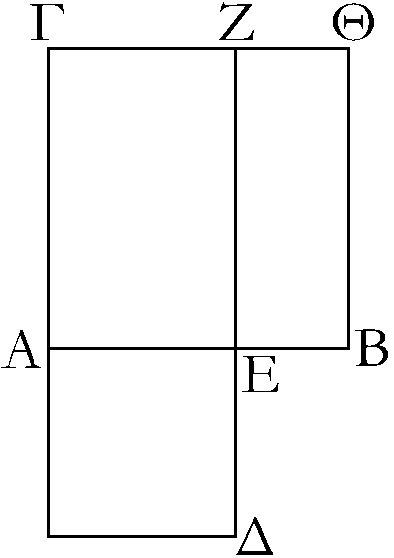
\includegraphics{Book06/fig30g.pdf}}

\gr{>'Εστω ἡ δοθεῖσα εὐθεῖα πεπερασμένη ἡ ΑΒ; δεῖ δὴ τὴν ΑΒ
εὐθεῖαν >άκρον καὶ μέσον λόγον τεμεῖν.}

\gr{Ἀναγεγράφθω ἀπὸ τῆξ ΑΒ τετράγωνον τὸ ΒΓ, καὶ παραβεβλήσθω
παρὰ τὴν ΑΓ τῶ| ΒΓ >ίσον παραλληλόγραμμον τὸ ΓΔ ὑπερβάλλον
ε>ίδει τῶ| ΑΔ ὁμοίῳ τῶ| ΒΓ.}

\gr{Τετράγωνον δέ ἐστι τὸ ΒΓ; τετράγωνον
 >άρα ἐστι καὶ τὸ ΑΔ.
καὶ ἐπεὶ >ίσον ἐστὶ τὸ ΒΓ τῶ| ΓΔ, κοινὸν ἀφῃρήσθω τὸ ΓΕ;
λοιπὸν >άρα τὸ ΒΖ λοιπῶ| τῶ| ΑΔ ἐστιν >ίσον. >έστι δὲ α\kern -.7pt  ὐτῶ| καὶ
ἰσογώνιον; τῶν ΒΖ, ΑΔ >άρα ἀντιπεπόνθασιν αἱ πλευραὶ
αἱ περὶ τὰξ >ίσαξ γωνίαξ; >έστιν >άρα ὡξ ἡ ΖΕ πρὸξ τὴν ΕΔ, ο<ύτωξ
ἡ ΑΕ πρὸξ τὴν ΕΒ. >ίση δὲ ἡ μὲν ΖΕ τῆ| ΑΒ, ἡ δὲ ΕΔ τῆ| ΑΕ.
>έστιν >άρα ὡξ ἡ ΒΑ πρὸξ τὴν ΑΕ, ο<ύτωξ ἡ ΑΕ πρὸξ τὴν ΕΒ. 
μείζων δὲ ἡ ΑΒ τῆξ ΑΕ; μείζων >άρα καὶ ἡ ΑΕ τῆξ ΕΒ.}

\gr{Ἡ >άρα ΑΒ εὐθεῖα >άκρον καὶ μέσον λόγον τέτμ\kern -.7pt  ηται κατὰ τὸ Ε,
καὶ τὸ μεῖζον α\kern -.7pt  ὐτῆξ τμ\kern -.5pt  ῆμά ἐστι τὸ ΑΕ; <όπερ >έδει
ποιῆσαι.}}

\ParallelRText{
\begin{center}
{\large Proposition 30}$^\dag$
\end{center}

To cut a given finite straight-line in extreme and
mean ratio.

% Removed epsf size command
\centerline{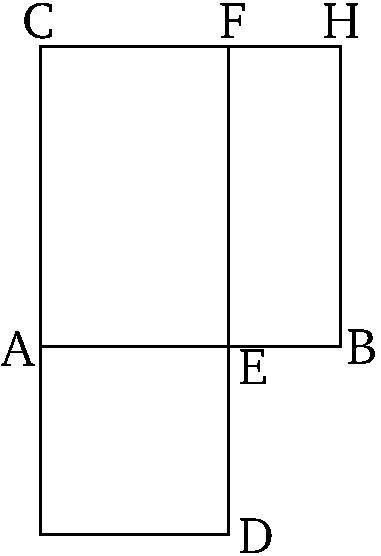
\includegraphics{Book06/fig30e.pdf}}

Let $AB$ be the given finite straight-line. So it is required to cut the straight-line $AB$ in extreme and mean ratio.

Let the square $BC$ be described on $AB$  [Prop. 1.46],
and let the parallelogram $CD$, equal to $BC$, be applied to $AC$,
overshooting by the figure $AD$ (which is) similar to $BC$ [Prop.~6.29].

And $BC$ is a square. Thus, $AD$ is also a square. And since $BC$ is equal to
$CD$, let (rectangle) $CE$ be subtracted from both. Thus, the remaining (rectangle) $BF$
is equal to the remaining (square) $AD$. And it is also equiangular to it. 
Thus, the sides of $BF$ and $AD$ about the equal angles are reciprocally proportional [Prop.~6.14]. 
Thus, as $FE$ is to $ED$, so $AE$ (is) to $EB$. And $FE$ (is) equal to $AB$, and $ED$ to
$AE$. Thus, as $BA$ is to $AE$, so $AE$ (is) to $EB$.  And $AB$ (is)
 greater than $AE$. Thus, $AE$ (is) also greater than $EB$ [Prop.~5.14].
 
 Thus, the straight-line $AB$ has been cut in extreme and mean ratio at $E$,
 and $AE$ is its greater piece. (Which is) the very thing it was required to
 do.}
\end{Parallel}
{\footnotesize\noindent$^\dag$ This method of cutting a straight-line
is sometimes called the ``Golden Section''---see Prop.~2.11.}

%%%%%%
% Prop 6.31
%%%%%%
\pdfbookmark[1]{Proposition 6.31}{pdf6.31}
\begin{Parallel}{}{} 
\ParallelLText{
\begin{center}
{\large \ggn{31}.}
\end{center}\vspace*{-7pt}

\gr{Ἐν τοῖξ ὀρθογωνίοιξ τριγώνοιξ τὸ ἀπὸ τῆξ τὴν ὀρθὴν γωνίαν
ὑποτεινούσηξ πλευρᾶξ ε>ῖδοξ >ίσον ἐστὶ τοῖξ ἀπὸ τῶν τὴν
ὀρθὴν γωνίαν περιεθουσῶν πλευρῶν ε>ίδεσι τοῖξ ὁμοίοιξ
τε καὶ ὁμοίωξ ἀναγραφομένοιξ.}

% Removed epsf size command
\centerline{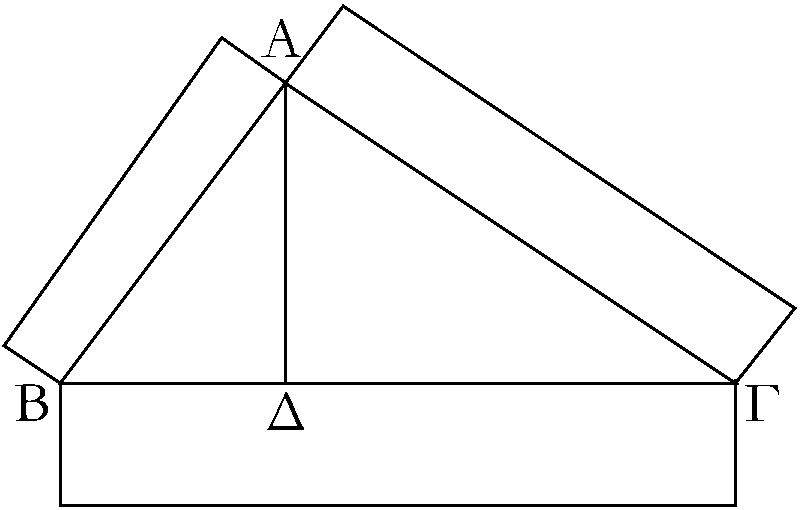
\includegraphics{Book06/fig31g.pdf}}

\gr{>'Εστω τρίγωνον ὀρθογώνιον τὸ ΑΒΓ ὀρθὴν >έθον τὴν ὑπὸ
ΒΑΓ γωνίαν; λέγω, <ότι τὸ ἀπὸ τῆξ ΒΓ ε>ῖδοξ >ίσον ἐστὶ 
τοῖξ ἀπὸ τῶν ΒΑ, ΑΓ ε>ίδεσι τοῖξ ὁμοίοιξ τε καὶ ὁμοίωξ
ἀναγραφομένοιξ.}

\gr{>'Ηθθω κάθετοξ ἡ ΑΔ.}

\gr{Ἐπεὶ ο>ῦν ἐν ὀρθογωνίῳ τριγώνῳ τῶ| ΑΒΓ ἀπὸ 
τῆξ πρὸξ τῶ| Α ὀρθῆξ γωνίαξ ἐπὶ τὴν ΒΓ βάσιν 
κάθετοξ >ῆκται ἡ ΑΔ, τὰ ΑΒΔ, ΑΔΓ πρὸξ τῆ| καθέτῳ 
τρίγωνα <όμοιά ἐστι τῶ| τε <όλῳ τῶ| ΑΒΓ καὶ ἀλλήλοιξ.
καὶ ἐπεὶ <όμοιόν ἐστι τὸ ΑΒΓ τῶ| ΑΒΔ, >έστιν >άρα ὡξ ἡ
ΓΒ πρὸξ τὴν ΒΑ, ο<ύτωξ ἡ ΑΒ πρὸξ τὴν ΒΔ. καὶ ἐπεὶ τρεῖξ
εὐθεῖαι ἀνάλογόν εἰσιν, >έστιν ὡξ ἡ πρώτη πρὸξ τὴν τρίτην,
ο<ύτωξ τὸ ἀπὸ τῆξ πρώτηξ ε>ῖδοξ πρὸξ τὸ ἀπὸ τῆξ δευτέραξ
τὸ <όμοιον καὶ ὁμοίωξ ἀναγραφόμενον. ὡξ >άρα ἡ ΓΒ πρὸξ τὴν
ΒΔ, ο<ύτωξ τὸ ἀπὸ τῆξ ΓΒ ε>ῖδοξ πρὸξ τὸ ἀπὸ τῆξ ΒΑ τὸ
<όμοιον καὶ ὁμοίωξ ἀναγραφόμενον. διὰ τὰ α\kern -.7pt  ὐτὰ δὴ καὶ
ὡξ ἡ ΒΓ πρὸξ τὴν ΓΔ, ο<ύτωξ τὸ ἀπὸ τῆξ ΒΓ ε>ῖδοξ πρὸξ
τὸ ἀπὸ τῆξ ΓΑ. <ώστε καὶ ὡξ ἡ ΒΓ πρὸξ τὰξ ΒΔ, ΔΓ, ο<ύτωξ
τὸ ἀπὸ τῆξ ΒΓ ε>ῖδοξ πρὸξ τὰ ἀπὸ τῶν ΒΑ, ΑΓ τὰ <όμοια
καὶ ὁμοίωξ ἀναγραφόμενα. >ίση δὲ ἡ ΒΓ ταῖξ ΒΔ, 
ΔΓ; >ίσον >άρα καὶ τὸ >άπὸ τῆξ ΒΓ ε>ῖδοξ τοῖξ ἀπὸ
τῶν ΒΑ, ΑΓ ε>ίδεσι τοῖξ ὁμοίοιξ τε καὶ ὁμοίωξ ἀναγραφομένοιξ.}

\gr{Ἐν >άρα τοῖξ ὀρθογωνίοιξ τριγώνοιξ τὸ ἀπὸ τῆξ τὴν ὀρθὴν γωνίαν
ὑποτεινούσηξ πλευρᾶξ ε>ῖδοξ >ίσον ἐστὶ τοῖξ ἀπὸ τῶν τὴν
ὀρθὴν γωνίαν περιεθουσῶν πλευρῶν ε>ίδεσι τοῖξ ὁμοίοιξ
τε καὶ ὁμοίωξ ἀναγραφομένοιξ; <όπερ >έδει δεῖχαι.}}

\ParallelRText{
\begin{center}
{\large Proposition 31}
\end{center}

In right-angled triangles, the figure (drawn)
on the side subtending the right-angle is equal to the (sum of the) similar, and similarly
described, figures on the sides surrounding the right-angle.

% Removed epsf size command
\centerline{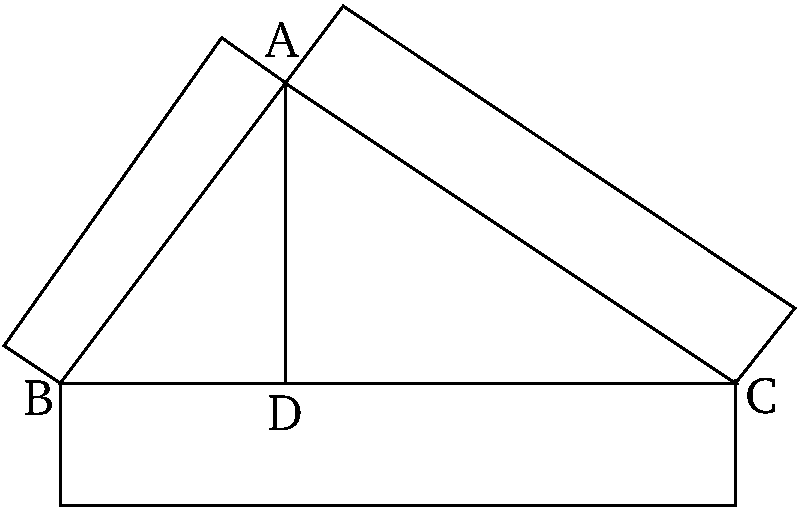
\includegraphics{Book06/fig31e.pdf}}

Let $ABC$ be a right-angled triangle having the angle $BAC$ a right-angle. I say
that the figure (drawn) on $BC$ is equal to the (sum of the) similar,
and similarly described, figures on $BA$ and $AC$.

Let the perpendicular $AD$ be drawn  [Prop. 1.12].

Therefore, since, in the right-angled triangle  $ABC$, the (straight-line) $AD$ has been drawn from the right-angle
at $A$ perpendicular to the base $BC$, the triangles $ABD$
and $ADC$ about the perpendicular are similar to the whole (triangle) $ABC$,
and to one another  [Prop.~6.8].
And since $ABC$ is similar to $ABD$, thus as $CB$ is to $BA$, so $AB$ (is) to
$BD$ [Def.~6.1]. And since three straight-lines
are proportional, as the first is to the third, so the figure (drawn) on the
first is to the similar, and similarly described, (figure) on the second 
[Prop.~6.19~corr.]. Thus, as $CB$ (is) to
$BD$, so the figure (drawn) on $CB$ (is) to the similar, and similarly
described, (figure) on $BA$. And so, for the same (reasons), as $BC$ (is) to
$CD$, so the figure  (drawn) on $BC$ (is) to the (figure) on $CA$. Hence,
also, as $BC$ (is) to $BD$ and $DC$, so the figure (drawn) on $BC$ (is) to
the (sum of the) similar, and similarly described, (figures) on $BA$ and $AC$ [Prop.~5.24].
And $BC$ is equal to $BD$ and $DC$. Thus, the figure (drawn) on $BC$
(is) also equal to the (sum of the) similar, and similarly described, figures
on $BA$ and $AC$ [Prop.~5.9].

Thus, in right-angled triangles, the figure (drawn)
on the side subtending the right-angle is equal to the (sum of the) similar, and similarly
described, figures on the sides surrounding the right-angle. (Which is)
the very thing it was required to show.\\~\\}
\end{Parallel}

%%%%%%
% Prop 6.32
%%%%%%
\pdfbookmark[1]{Proposition 6.32}{pdf6.32}
\begin{Parallel}{}{} 
\ParallelLText{
\begin{center}
{\large \ggn{32}.}
\end{center}\vspace*{-7pt}

\gr{Ἐὰν δύο τρίγωνα συντεθῆ| κατὰ μίαν γωνίαν τὰξ δύο πλευρὰξ ταῖξ
δυσὶ πλευραῖξ ἀνάλογον >έθοντα <ώστε τὰξ ὁμολόγουξ α\kern -.7pt  ὐτῶν
πλευρὰξ  καὶ παραλλήλουξ ε>ῖναι, αἱ λοιπαὶ τῶν τριγώνων πλευραὶ
ἐπ> εὐθείαξ >έσονται.}

% Removed epsf size command
\centerline{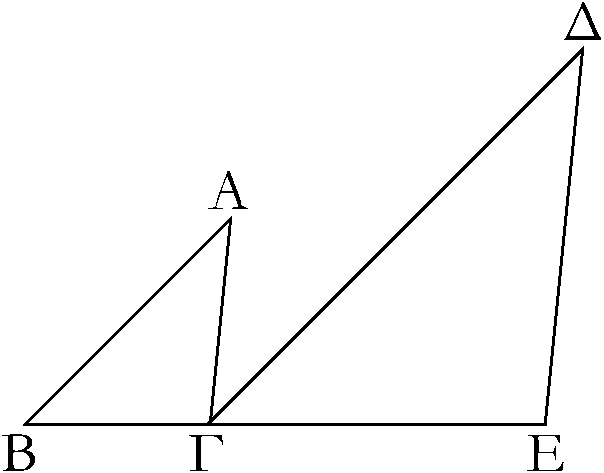
\includegraphics{Book06/fig32g.pdf}}

\gr{>'Εστω δύο τρίγωνα τὰ ΑΒΓ, ΔΓΕ τὰξ δύο πλευρὰξ τὰξ ΒΑ, ΑΓ
ταῖξ δυσὶ πλευραῖξ ταῖξ ΔΓ, ΔΕ ἀνάλογον >έθοντα, ὡξ μὲν
τὴν ΑΒ πρὸξ τὴν ΑΓ, ο<ύτωξ τὴν ΔΓ πρὸξ τὴν ΔΕ, παράλληλον δὲ τὴν μὲν ΑΒ τῆ|
ΔΓ, τὴν δὲ ΑΓ τῆ| ΔΕ; λέγω, <ότι ἐπ> εὐθείαξ ἐστὶν ἡ ΒΓ
τῆ| ΓΕ.}

\gr{Ἐπεὶ γὰρ παράλληλόξ ἐστιν ἡ ΑΒ τῆ| ΔΓ, καὶ εἰξ α\kern -.7pt  ὐτὰξ
ἐμπέπτωκεν εὐθεῖα ἡ ΑΓ, αἱ ἐναλλὰχ γωνίαι αἱ ὑπὸ ΒΑΓ,
ΑΓΔ >ίσαι ἀλλήλαιξ εἰσίν. διὰ τὰ α\kern -.7pt  ὐτὰ δὴ καὶ ἡ ὑπὸ ΓΔΕ
τῆ| ὑπὸ ΑΓΔ >ίση ἐστίν. <ώστε καὶ ἡ ὑπὸ ΒΑΓ τῆ| ὑπὸ
ΓΔΕ ἐστιν >ίση. καὶ ἐπεὶ δύο τρίγωνά ἐστι τὰ ΑΒΓ, ΔΓΕ
μίαν γωνίαν τὴν πρὸξ τῶ| Α μιᾶ| γωνίᾳ τῆ| πρὸξ τῶ| Δ >ίσην
>έθοντα, περὶ δὲ τὰξ >ίσαξ γωνίαξ τὰξ πλευρὰξ ἀνάλογον,
ὡξ τὴν ΒΑ πρὸξ τὴν ΑΓ, ο<ύτωξ τὴν ΓΔ πρὸξ τὴν ΔΕ,
ἰσογώνιον >άρα ἐστὶ τὸ ΑΒΓ τρίγωνον τῶ| ΔΓΕ τριγώνῳ; >ίση
>άρα ἡ ὑπὸ ΑΒΓ γωνία τῆ| ὑπὸ ΔΓΕ. ἐδείθθη
δὲ καὶ ἡ ὑπὸ ΑΓΔ τῆ| ὑπὸ ΒΑΓ >ίση; <όλη >άρα ἡ ὑπὸ
ΑΓΕ δυσὶ ταῖξ ὑπὸ ΑΒΓ, ΒΑΓ >ίση ἐστίν. κοινὴ προσκείσθω ἡ ὑπὸ
ΑΓΒ; αἱ >άρα ὑπὸ  ΑΓΕ, ΑΓΒ ταῖξ ὑπὸ ΒΑΓ, ΑΓΒ, ΓΒΑ
>ίσαι εἰσίν. ἀλλ> αἱ ὑπὸ ΒΑΓ, ΑΒΓ, ΑΓΒ
   δυσὶν
ὀρθαῖξ >ίσαι εἰσίν; καὶ αἱ ὑπὸ ΑΓΕ, ΑΓΒ >άρα δυσὶν ὀρθαῖξ
>ίσαι εἰσίν. πρὸξ δή τινι εὐθείᾳ τῆ| ΑΓ καὶ τῶ| πρὸξ α\kern -.5pt  ὐτῆ|
σημείῳ τῶ| Γ δύο εὐθεῖαι αἱ ΒΓ, ΓΕ μ\kern -.3pt  ὴ ἐπὶ τὰ α\kern -.7pt  ὐτὰ μέρη
κείμεναι τὰξ ἐφεχῆξ γωνάιξ τὰξ ὑπὸ ΑΓΕ, ΑΓΒ δυσὶν
ὀρθαῖξ >ίσαξ ποιοῦσιν; ἐπ> εὐθείαξ >άρα ἐστὶν ἡ ΒΓ τῆ| ΓΕ.}

\gr{Ἐὰν >άρα δύο τρίγωνα συντεθῆ| κατὰ μίαν γωνίαν τὰξ δύο πλευρὰξ ταῖξ
δυσὶ πλευραῖξ ἀνάλογον >έθοντα <ώστε τὰξ ὁμολόγουξ α\kern -.7pt  ὐτῶν
πλευρὰξ  καὶ παραλλήλουξ ε>ῖναι, αἱ λοιπαὶ τῶν τριγώνων πλευραὶ
ἐπ> εὐθείαξ >έσονται; <όπερ >έδει δεῖχαι.}}

\ParallelRText{
\begin{center}
{\large Proposition 32}
\end{center}

If two triangles,
having two sides proportional to two sides, are placed together at a single angle such that the corresponding 
sides are also parallel, (then) the remaining sides of the triangles will
be straight-on (with respect to one another).

% Removed epsf size command
\centerline{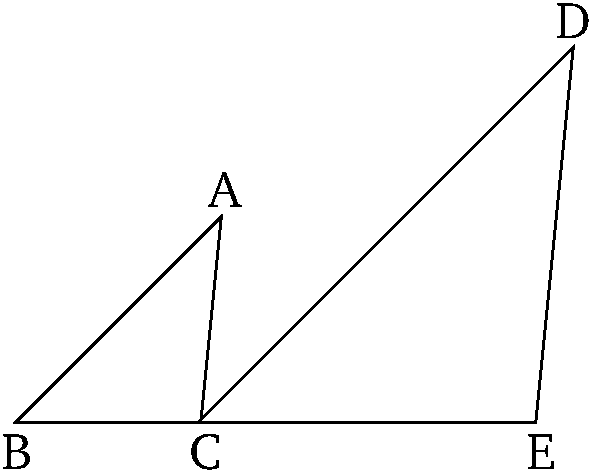
\includegraphics{Book06/fig32e.pdf}}

Let $ABC$ and $DCE$ be two triangles having the two sides $BA$ and $AC$
proportional to the two sides $DC$ and $DE$---so that as $AB$ (is) to $AC$, so
$DC$ (is) to $DE$---and (having side) $AB$ parallel to $DC$, and $AC$ to $DE$. I say that (side) $BC$
is straight-on to $CE$.

For since $AB$ is parallel to $DC$, and the straight-line $AC$ has fallen across them, the alternate angles $BAC$ and $ACD$ are equal to one another  [Prop.~1.29]. So, for the same (reasons), $CDE$ is also equal to $ACD$. 
And, hence, $BAC$ is equal to $CDE$. And since $ABC$ and $DCE$ are two triangles
having the one angle at $A$ equal to the one angle at $D$, and the sides about the
equal angles proportional, (so that) as $BA$ (is) to $AC$, so $CD$ (is) to $DE$, triangle $ABC$ is thus equiangular to triangle $DCE$ [Prop.~6.6].  Thus, angle $ABC$ is equal to $DCE$.
And (angle) $ACD$ was also shown (to be) equal to $BAC$. Thus, the whole
(angle) $ACE$ is equal to the two (angles) $ABC$ and $BAC$. Let $ACB$ 
be added to both. Thus, $ACE$ and $ACB$ are equal to $BAC$, $ACB$,  and
$CBA$. But, $BAC$, $ABC$, and $ACB$ are equal to two right-angles  [Prop.~1.32]. Thus, $ACE$ and $ACB$ are also equal to two right-angles.
Thus, the two straight-lines $BC$ and $CE$, not lying on the same side, 
make  adjacent angles $ACE$ and $ACB$ (whose sum is) equal to two right-angles with some straight-line $AC$,  at the
point $C$ on it. Thus, $BC$ is straight-on to
$CE$  [Prop.~1.14].

Thus, if  two triangles,
having two sides proportional to two sides, are placed together at a single angle such that the corresponding 
sides are also parallel, (then) the remaining sides of the triangles will
be straight-on (with respect to one another). (Which is) the very thing it
was required to show.}
\end{Parallel}

%%%%%%
% Prop 6.33
%%%%%%
\pdfbookmark[1]{Proposition 6.33}{pdf6.33}
\begin{Parallel}{}{} 
\ParallelLText{
\begin{center}
{\large \ggn{33}.}
\end{center}\vspace*{-7pt}

\gr{Ἐν τοῖξ >ίσοιξ κύκλοιξ αἱ γωνίαι τὸν α\kern -.7pt  ὐτὸν >έθουσι λόγον ταῖξ
περιφερείαιξ, ἐφ> <ῶν βεβήκασιν, ἔαν τε πρὸξ τοῖξ κέντροιξ
ἔαν τε πρὸξ ταῖξ περιφερείαιξ >ῶσι βεβηκυῖαι.}

\gr{>'Εστωσαν >ίσοι κύκλοι οἱ ΑΒΓ, ΔΕΖ, καὶ πρὸξ
μὲν τοῖξ κέντροιξ α\kern -.7pt  ὐτῶν τοῖξ Η, Θ γωνίαι >έστωσαν αἱ ὑπὸ
ΒΗΓ, ΕΘΖ, πρὸξ δὲ ταῖξ περιφερείαιξ αἱ ὑπὸ ΒΑΓ, ΕΔΖ;
λέγω, <ότι ἐστὶν ὡξ ἡ ΒΓ περιφέρεια πρὸξ τὴν
ΕΖ περιφέρειαν, ο<ύτωξ <ή τε ὑπὸ ΒΗΓ γωνία πρὸξ τὴν ὑπὸ
ΕΘΖ καὶ ἡ ὑπὸ ΒΑΓ πρὸξ τὴν ὑπὸ ΕΔΖ.}

% Removed epsf size command
\centerline{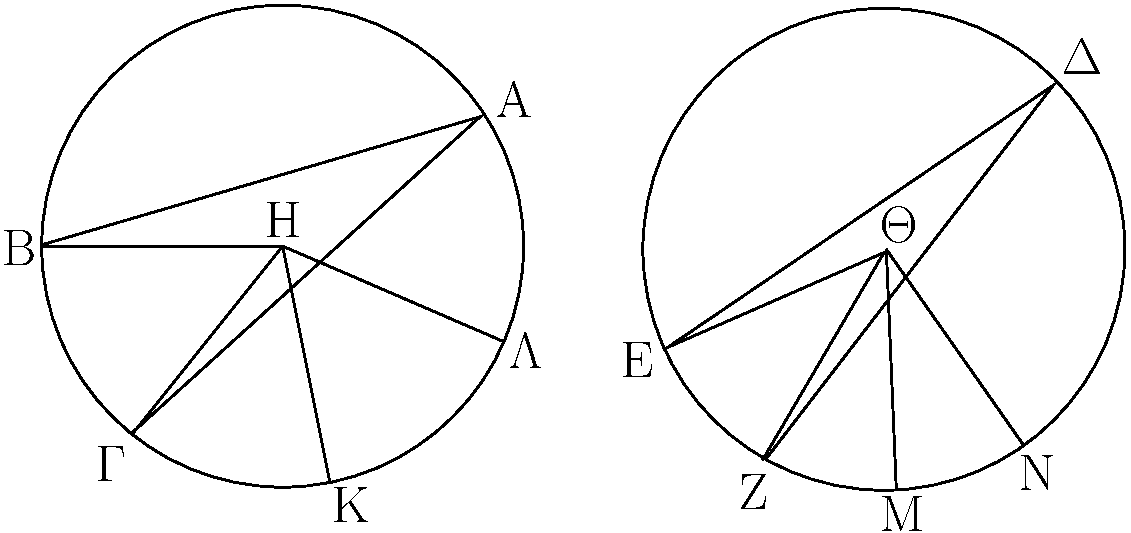
\includegraphics{Book06/fig33g.pdf}}

\gr{Κείσθωσαν γὰρ τῆ| μὲν ΒΓ περιφερείᾳ >ίσαι κατὰ τὸ ἑχῆξ ὁσαιδηποτοῦν αἱ ΓΚ, ΚΛ, τῆ| δὲ ΕΖ περιφερείᾳ >ίσαι ὁσαιδηποτοῦν
αἱ ΖΜ, ΜΝ, καὶ ἐπεζεύθθωσαν αἱ ΗΚ, ΗΛ, ΘΜ, ΘΝ.}

\gr{Ἐπεὶ ο>ῦν >ίσαι εἰσὶν αἱ ΒΓ, ΓΚ, ΚΛ περιφέρειαι ἀλλήλαιξ, >ίσαι εἰσὶ καὶ αἱ ὑπὸ ΒΗΓ, ΓΗΚ, ΚΗΛ
γωνίαι ἀλλήλαιξ; ὁσαπλασίων >άρα ἐστὶν ἡ ΒΛ περιφέρεια τῆξ
ΒΓ, τοσαυταπλασίων ἐστὶ καὶ ἡ ὑπὸ ΒΗΛ γωνία τῆξ ὑπὸ ΒΗΓ. διὰ
τὰ α\kern -.7pt  ὐτὰ δὴ καὶ ὁσαπλασίων  ἐστὶν ἡ ΝΕ περιφέρεια τῆξ ΕΖ,
τοσαυταπλασίων ἐστὶ καὶ ἡ ὑπὸ ΝΘΕ γωνία τῆξ ὑπὸ ΕΘΖ. εἰ
>άρα >ίση ἐστὶν ἡ ΒΛ περιφέρεια τῆ| ΕΝ περιφερείᾳ, >ίση
ἐστὶ καὶ γωνία ἡ ὑπὸ ΒΗΛ τῆ| ὑπὸ ΕΘΝ, καὶ εἰ
μείζων ἐστὶν ἡ ΒΛ περιφέρεια τῆξ ΕΝ περιφερείαξ, μείζων
ἐστὶ καὶ ἡ ὑπὸ ΒΗΛ γωνία τῆξ ὑπὸ ΕΘΝ, καὶ εἰ
ἐλάσσων, ἐλάσσων. τεσσάρων δὴ >όντων μεγεθῶν, δύο μὲν
περιφερειῶν τῶν ΒΓ, ΕΖ, δύο δὲ γωνιῶν τῶν ὑπὸ ΒΗΓ, ΕΘΖ,
ε>ίληπται τῆξ μὲν ΒΓ περιφερείαξ  καὶ τῆξ ὑπὸ ΒΗΓ γωνίαξ 
ἰσάκιξ πολλαπλασίων <ή τε ΒΛ περιφέρεια καὶ ἡ ὑπὸ ΒΗΛ
γωνία, τῆξ δὲ ΕΖ περιφερείαξ καὶ τῆξ ὑπὸ ΕΘΖ γωνίαξ <ή 
τε ΕΝ περιφέρια καὶ ἡ ὑπὸ ΕΘΝ γωνία. καὶ δέδεικται, <ότι
εἰ ὑπερέθει ἡ ΒΛ περιφέρεια τῆξ ΕΝ περιφερείαξ, ὑπερέθει
καὶ ἡ ὑπὸ ΒΗΛ γωνία τῆξ ὑπο ΕΘΝ γωνίαξ, καὶ εἰ >ίση, >ίση,
καὶ εἰ ἐλάσσων, ἐλάσσων.  >έστιν >άρα, ὡξ ἡ ΒΓ περιφέρεια πρὸξ τὴν
ΕΖ, ο<ύτωξ ἡ ὑπὸ ΒΗΓ γωνία πρὸξ τὴν ὑπὸ ΕΘΖ. ἀλλ>
ὡξ ἡ ὑπὸ ΒΗΓ γωνία πρὸξ τὴν ὑπὸ ΕΘΖ, ο<ύτωξ
ἡ ὑπὸ ΒΑΓ
 πρὸξ τὴν ὑπὸ ΕΔΖ. διπλασία γὰρ ἑκατέρα
ἑκατέραξ. καὶ  ὡξ >άρα ἡ ΒΓ περιφέρεια πρὸξ τὴν ΕΖ
περιφέρειαν, ο<ύτωξ <ή τε ὑπὸ ΒΗΓ γωνία πρὸξ τὴν ὑπὸ
ΕΘΖ καὶ ἡ ὑπὸ ΒΑΓ πρὸξ τὴν ὑπὸ ΕΔΖ.}

\gr{Ἐν >άρα τοῖξ >ίσοιξ κύκλοιξ αἱ γωνίαι τὸν α\kern -.7pt  ὐτὸν >έθουσι λόγον ταῖξ
περιφερείαιξ, ἐφ> <ῶν βεβήκασιν, ἔαν τε πρὸξ τοῖξ κέντροιξ
ἔαν τε πρὸξ ταῖξ περιφερείαιξ >ῶσι βεβηκυῖαι; <όπερ >έδει
δεῖχαι.}}

\ParallelRText{
\begin{center}
{\large Proposition 33}
\end{center}

In equal circles,  angles have the same ratio
as the (ratio of the) circumferences on which they stand, whether they are standing at
the centers (of the circles) or at the circumferences.

Let $ABC$ and $DEF$ be equal circles, and let $BGC$ and $EHF$ be angles
at their centers, $G$ and $H$ (respectively), and $BAC$ and $EDF$ (angles)
at their circumferences. I say that as circumference $BC$ is to circumference
$EF$, so angle $BGC$ (is) to $EHF$, and (angle) $BAC$ to $EDF$.\\

% Removed epsf size command
\centerline{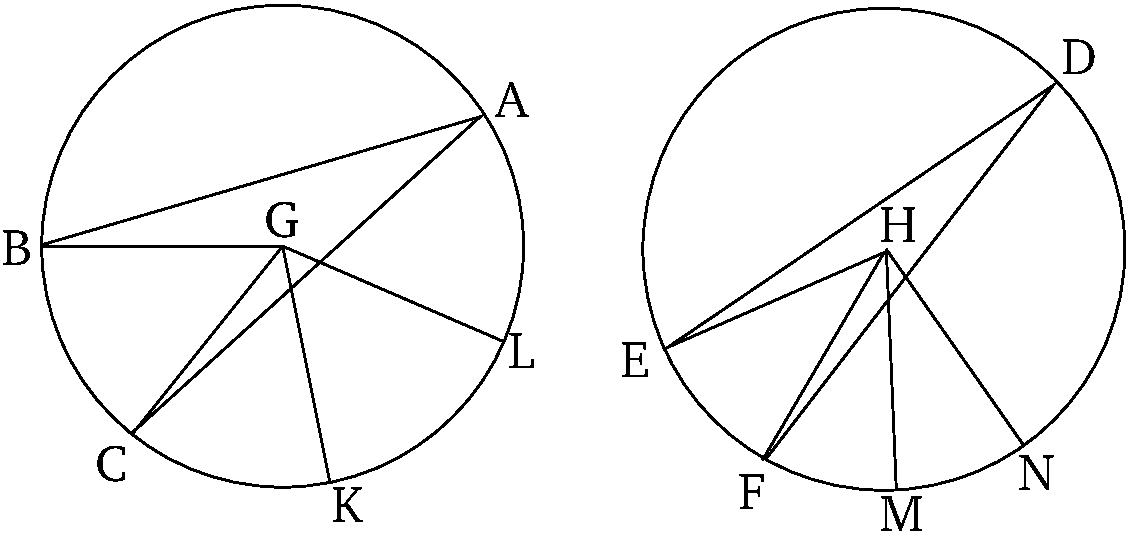
\includegraphics{Book06/fig33e.pdf}}

For let any number whatsoever of consecutive (circumferences), $CK$ and
$KL$, be made equal to circumference $BC$, and any number whatsoever, $FM$ and $MN$, to circumference $EF$. And let $GK$, $GL$, $HM$, and $HN$ be
joined.

Therefore, since circumferences $BC$, $CK$, and $KL$ are equal to one
another, angles $BGC$, $CGK$, and $KGL$ are also equal to
one another [Prop.~3.27].  Thus, as many times as circumference $BL$
is (divisible) by $BC$, so many times is angle $BGL$ also
(divisible) by $BGC$. And so, for the same (reasons), as many times as
circumference $NE$ is (divisible) by $EF$, so many times is
angle $NHE$ also (divisible) by $EHF$. Thus, if circumference $BL$
is equal to circumference $EN$ (then) angle $BGL$ is also equal to $EHN$ [Prop.~3.27], and
if circumference $BL$ is greater than circumference $EN$ (then) angle
$BGL$ is also greater than $EHN$,$^\dag$ and if ($BL$ is) less (than $EN$ then $BGL$ is also) less (than $EHN$). So there are four magnitudes, two circumferences
$BC$ and $EF$, and two angles $BGC$ and $EHF$. And equal multiples
have been taken of circumference $BC$ and angle $BGC$, (namely)
circumference $BL$ and angle $BGL$, and of circumference $EF$ and angle
$EHF$, (namely) circumference $EN$ and angle $EHN$. And it has been
shown that if circumference $BL$ exceeds circumference
$EN$ (then) angle $BGL$ also exceeds angle $EHN$, and if ($BL$ is) equal (to $EN$
then $BGL$ is also) equal (to $EHN$), and if ($BL$ is) less (than $EN$
then $BGL$ is also) less (than $EHN$). Thus, as circumference
$BC$ (is) to $EF$, so angle $BGC$ (is) to $EHF$ [Def.~5.5]. But as
angle $BGC$ (is) to $EHF$, so  (angle) $BAC$ (is) to $EDF$ [Prop.~5.15]. For the former (are) double the
latter (respectively) [Prop.~3.20]. Thus, also, as circumference $BC$ (is)
to circumference $EF$, so  angle $BGC$ (is) to $EHF$, and $BAC$ to $EDF$.

Thus, in equal circles,  angles have the same ratio
as the (ratio of the) circumferences on which they stand, whether they are standing at
the centers (of the circles) or at the circumferences. (Which is) the very thing it was required to show.}
\end{Parallel}
{\footnotesize\noindent$^\dag$ This is a straight-forward generalization of Prop.~3.27}
